\documentclass[10pt,twocolumn]{article} 
\usepackage{simpleConference}
\usepackage{fancyhdr}
\usepackage{amsmath,amsfonts,amssymb,graphicx}
\usepackage{subcaption}   % 使用子图形
\usepackage{indentfirst} % 中文段落首行缩进
\usepackage{bm}          % 公式中的粗体字符(用命令\boldsymbol)
\usepackage{indentfirst} % 中文首段缩进
\usepackage{abstract}    % 2栏文档,一栏摘要及关键字宏包
\usepackage{amsthm}      % 使用定理
\usepackage{booktabs}    % 使用表格
\usepackage{siunitx}
\usepackage{tikz}
\usepackage{enumitem}
\usepackage{titlesec}
\usepackage{times}
\usepackage{wasysym}
\usepackage{pifont}
\usepackage{ccaption}
\usepackage{float}
\usepackage{calc}
\usetikzlibrary{calc}
\usetikzlibrary{circuits.ee.IEC}
% 在导言区添加 circuitikz 包
\usepackage{circuitikz}
\usepackage{environ}
\usepackage{lmodern}
\usepackage{anyfontsize}
\usepackage{hyperref}
\usepackage{tabu}
\usepackage{tabularx}
\usepackage{multirow}
\usepackage{multicol}
\usepackage{longtable}
\usepackage{makecell}
\usepackage{graphicx}
\usepackage{amssymb}
\usepackage{ragged2e}
\usepackage{url,hyperref}
\usepackage[
    backend=biber,
    style=nature,
]{biblatex}

\newcommand*{\effXsecDPS}{\sigma_{\text{eff,DPS}}}
\newcommand*{\effXsecTPS}{\sigma_{\text{eff,TPS}}}
\newcommand*{\GeV}{~\text{GeV}}
\newcommand*{\GeVc}{~\text{GeV/c}}
\newcommand*{\GeVcs}{~\text{GeV}\text{c}^2}
\newcommand*{\parFlav}{\texttt{partonFlavour}}
\newcommand*{\hadFlav}{\texttt{hadronFlavour}}

\renewcommand{\arraystretch}{1.2}

\addbibresource{mainTemplatePDF.bib}

\begin{document}

\title{Integration of GHS Algorithm for Jet Flavour Definition in CMS Offline Software (CMSSW)}

\author{Chi Wang \\
\\
Tsinghua University \\
\today
\\
\\
\texttt{chi.w@cern.ch} \\
}

\maketitle
\thispagestyle{empty}

\begin{abstract}

Jets, collimated sprays of particles resulting from the hadronization of quarks and gluons, are fundamental objects in high-energy physics experiments such as those conducted at the Large Hadron Collider (LHC). The ability to accurately identify the flavour of jets, particularly those originating from heavy-flavour quarks (b and c), is crucial for a wide range of physics analyses, including studies of the Higgs boson, top quark properties, and searches for new physics phenomena. Traditional jet flavour definitions used in the CMS experiment's Offline Software (CMSSW) framework are known to be infrared and collinear (IRC) unsafe, leading to ambiguities and divergences in theoretical calculations, hindering precise comparisons between experimental measurements and theoretical predictions.

This report details the successful integration of the IRC-safe GHS jet flavour algorithm into the CMSSW framework. The integration involved interfacing with the external $\texttt{fastjet-contrib}$ library, developing a ghost-clustering method for associating partons with jets, and designing a compact storage format for jet flavour information in NanoAOD files. A comprehensive validation using simulated $t\bar{t}$ events demonstrates that the GHS algorithm provides physically sensible results consistent with conventional definitions while avoiding their pitfalls. The implementation is being prepared for inclusion in an official CMSSW release, paving the way for its adoption in future CMS physics analyses.

\end{abstract}

\section{Introduction}
\label{sec:intro}

\subsection{Jets as Probes for Parton-level Physics at the LHC}
\label{sec:intro-jets}

Quarks, the fundamental building blocks that make up protons, neutrons and other hadrons to form most of the visible matter, come in six distinct flavours with different masses: up (u), down (d), strange (s), charm (c), bottom (b), and top (t), and interact primarily via the strong force mediated by gluons, a fundamental interaction described by the theory of Quantum Chromodynamics (QCD).

In the high-energy environment of proton-proton collisions at the LHC, quarks and gluons, collectively referred to as partons, are produced in various physics processes of interest. Due to a property of the strong force known as "colour confinement," these partons cannot be observed directly. Instead, they immediately undergo a series of complex processes including parton showering and hadronization, to form collimated sprays of detectable particles referred to as jets. By studying the properties of these jets, physicists can infer the kinematics and identity of the underlying partons, thus gaining insight into the fundamental interactions at play.

The ability to predict and to identify jets and their flavour, particularly identifying those originating from heavy-flavour quarks (b and c), is essential for many frontier experimental analyses, including studies of the Higgs boson (e.g., $H \rightarrow b\bar{b}$), precision measurements of the top quark, and searches for new particles that may preferentially decay to heavy-flavour quarks.

\subsection{The CMS Experiment at the LHC} %[TODO: citation, dissection]
\label{sec:intro-cms}

The Compact Muon Solenoid (CMS) is one of the largest and most important experiments at the LHC, designed to investigate a wide range of physics phenomena, from the Higgs boson to potential new physics beyond the Standard Model. \cite{CMS_JINST_2008, acostaCMSPhysicsTDR2006} The detector itself measures 21 meters in length and 15 meters in diameter, with a total weight of approximately 14,000 tonnes. Its sophisticated sub-detectors (shown in Figure \ref{fig:CMS_disection}), including a high-precision silicon tracker, high-granularity calorimeters, and a powerful muon system, enable the detailed reconstruction of particles produced in high-energy collisions.

\begin{figure*}[!bth]
    \centering
    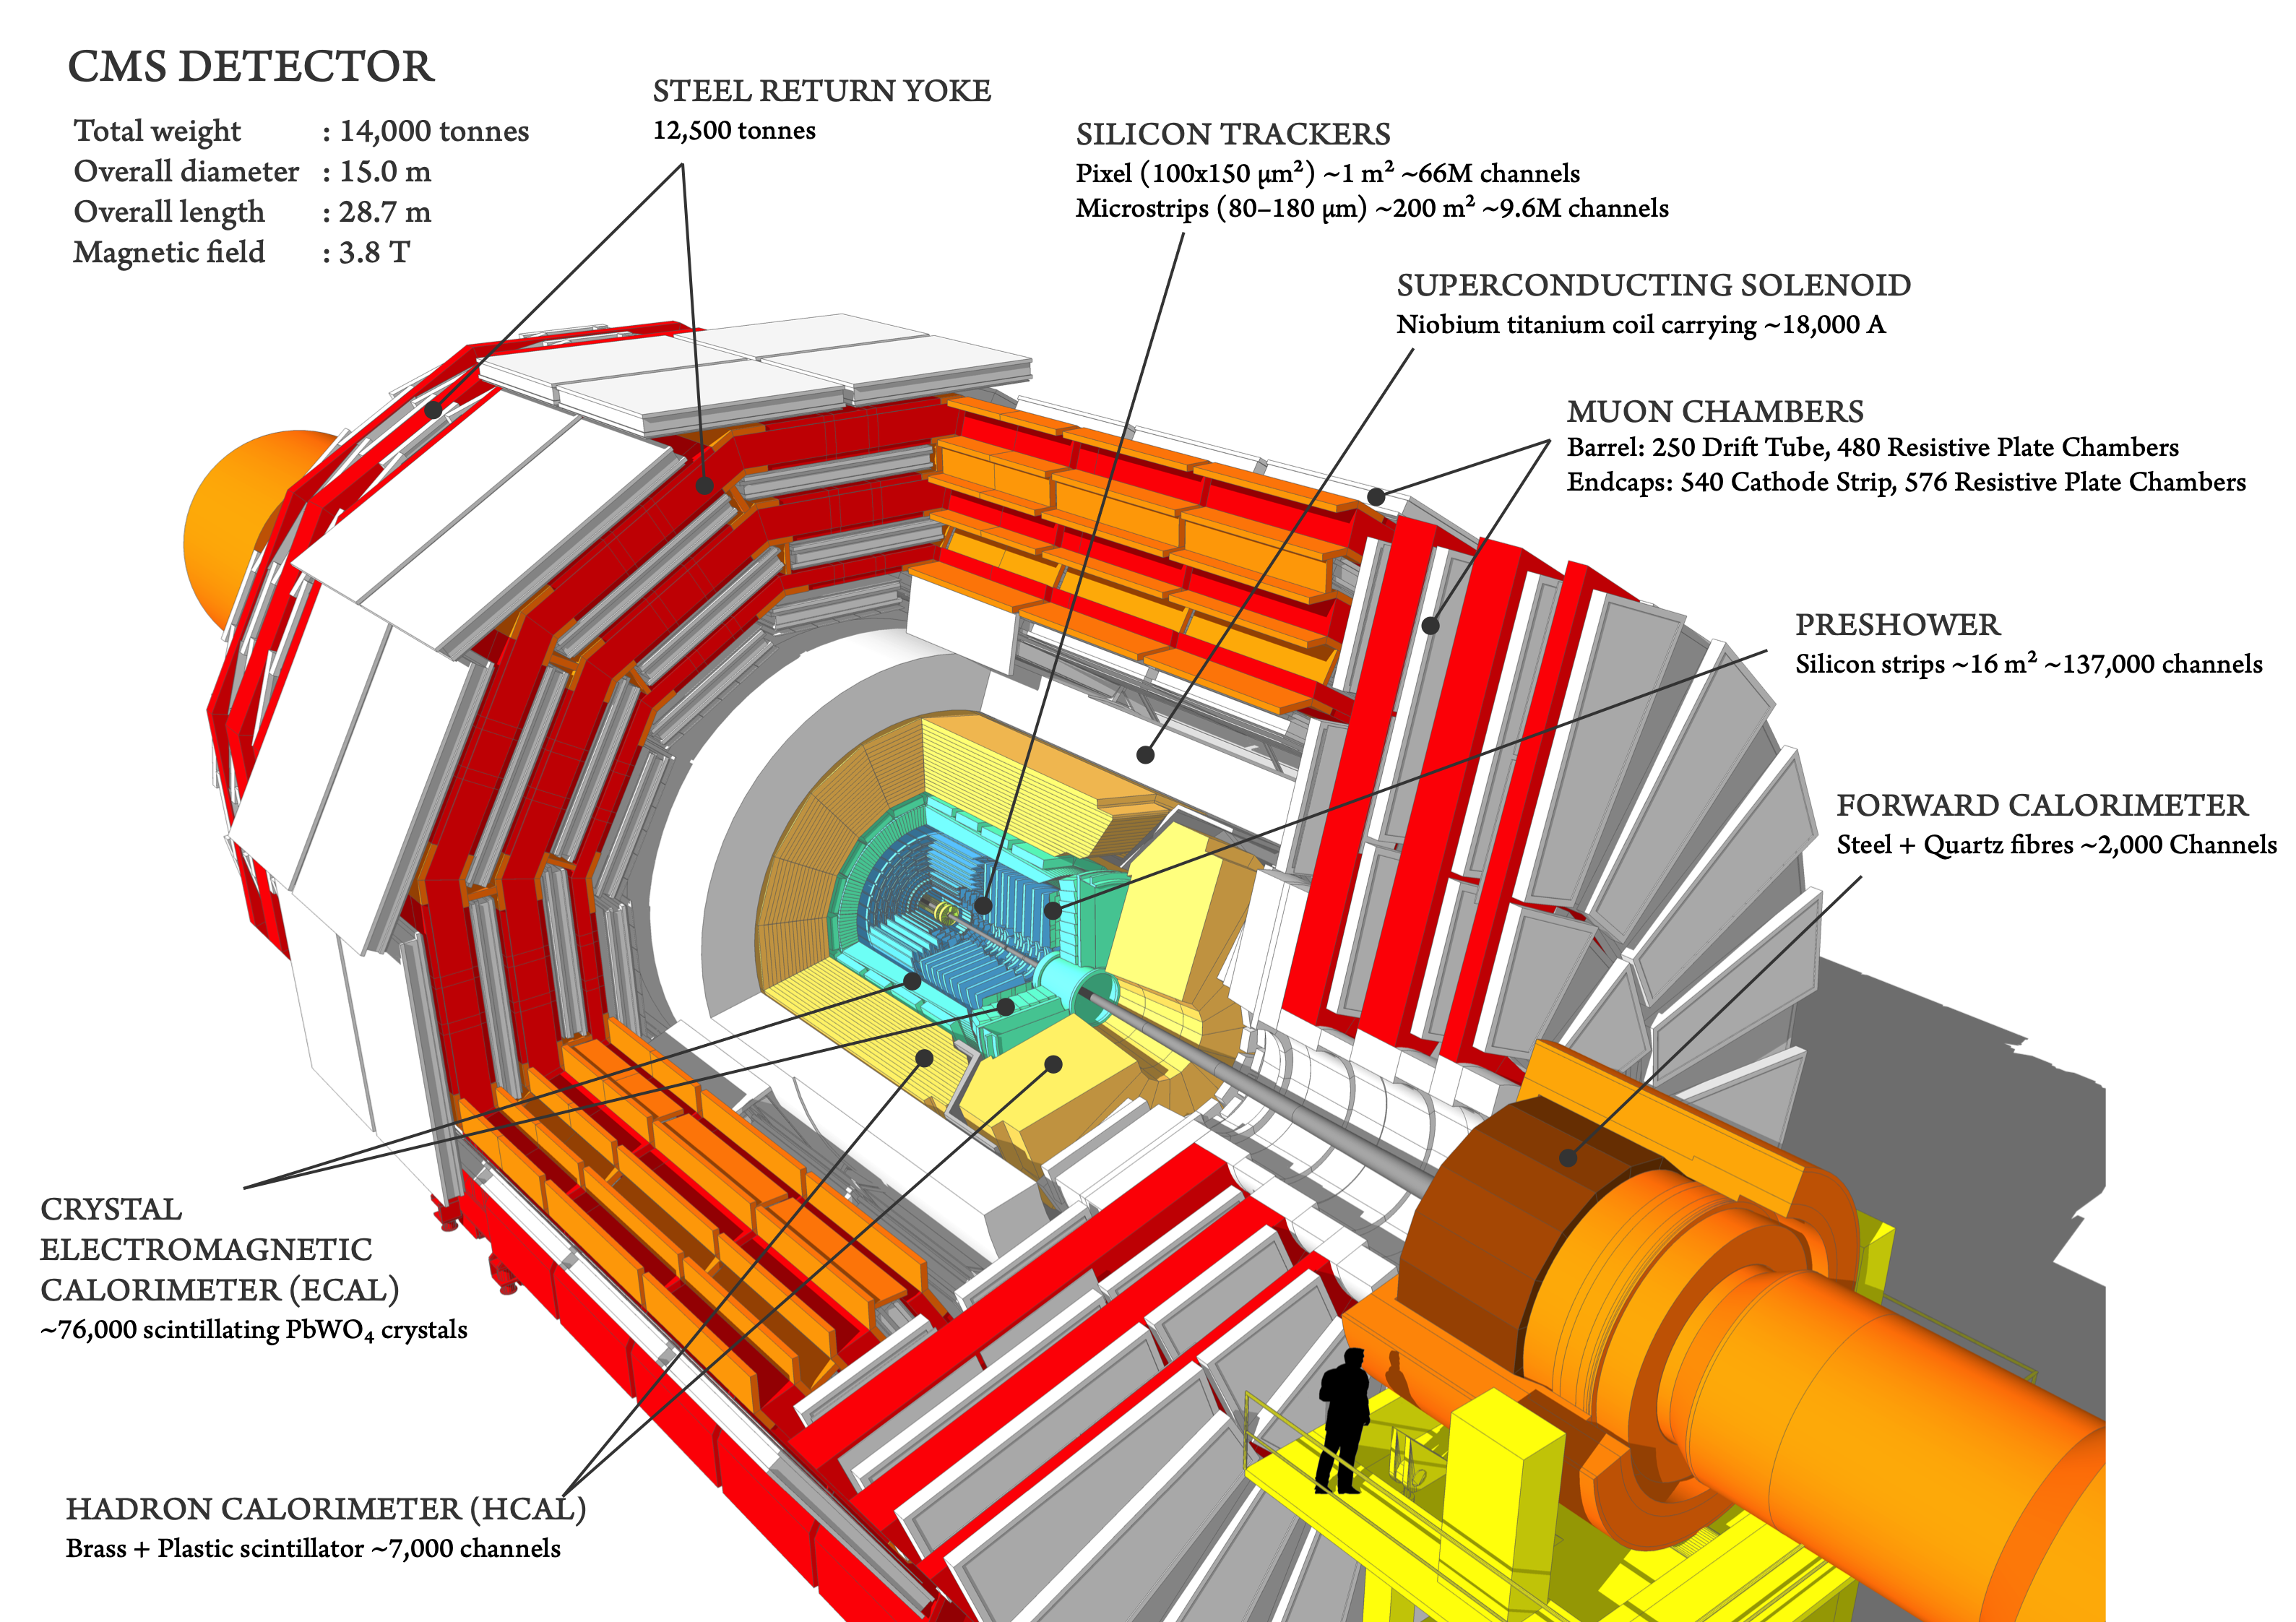
\includegraphics[width=0.70\textwidth]{images/CMS_disection_Run2.png}
    \caption{A schematic dissection of the CMS detector, showing its various sub-detectors and their arrangement around the collision point.\cite{CMS_CUTAWAY_DIAGRAM}}
    \label{fig:CMS_disection}
\end{figure*}

All data processing, from initial event reconstruction to final physics analysis, is managed within the CMS Offline Software (CMSSW), a flexible framework based on C++. 

\subsection{Jet Definitions and Jet Flavour Definitions}
\label{sec:intro-jetdef}

A precise and robust definition of jet and its flavour is essential for establishing an unambiguous comparison between theoretical predictions and experimental measurements, given the complex evolution of quarks and gluons into final-state jets. The foundational requirements for such a definition were outlined in the 1990 "Snowmass Accord"\cite{bergerStandardizationJetDefinitions1992_Snowmass1990}:

\begin{enumerate}
    \item Simple to implement in an experimental analysis;
    \item Simple to implement in the theoretical calculation;
    \item Defined at any order of perturbation theory;
    \item Yields finite cross section at any order of perturbation theory;
    \item Yields a cross section that is relatively insensitive to hadronization.
\end{enumerate}

Modern jet definitions satisfying such requirements have been proposed. Notably, the anti-$k_T$ algorithm \cite{ANTIKT_2008}, has been implemented in the FastJet library \cite{FASTJET_EPJC_2012} with wide adoption in the LHC experiments for jet clustering.

However, the conventional flavour definitions used in the CMSSW are known to be IRC-unsafe. They rely on a simple geometric matching between a reconstructed jet and the nearest heavy-flavour parton ("$\parFlav$") or hadron ("$\hadFlav$")in the simulated event record. This pragmatic approach has a critical flaw: a jet's flavour can be incorrectly changed in higher-order QCD processes, such as a soft gluon splitting into a heavy-quark pair ($g \rightarrow c\bar{c}$ or $g \rightarrow b\bar{b}$) far from the jet's core, leading to divergences in theoretical calculations and hindering high-precision comparisons between theory and experiment.

\subsection{The GHS Algorithm and Other IRC-safe Jet Flavour Definitions}
\label{sec:intro-ghs}

The last few years have seen a "flavour revolution" in theoretical jet physics, with the development of several new algorithms designed to assign jet flavour in an IRC-safe manner \cite{JETFLAVALGO_COMP_2005}. One of the most promising is the flavour dressing algorithm \cite{GHS_V2_2024} developed by Gauld, Huss, and Stagnitto. For brevity, we refer to this algorithm as the GHS algorithm in the following discussion.

The GHS algorithm assigns the flavour to the jet based on the associated partons using a flavour-aware combination procedure. The key steps of the GHS algorithm are as follows:
\begin{enumerate}
    \item Creating a set $\mathcal{D}$ of such distance measures:
    \begin{enumerate}
        \item For each unordered pair of particles $p_i$ and $p_j$, add the distance measure $d_{p_ip_j}$ if either both particles are flavoured, or at least one particle is unflavoured and $p_i$ and $p_j$ are associated with the same jet.
        \item If the particle $p_i$ is associated to jet $j_k$, add the distance measure $d_{p_ij_k}$. In a hadron collider environment, the beam distances $d_{p_iB^\pm}$ should be added if $p_i$ is not associated to any jet.
    \end{enumerate}
    \item While $\mathcal{D}$ is not empty, select the pairing with the smallest distance measure:
    \begin{enumerate}
        \item If the smallest distance is $d_{p_ip_j}$, merge particles $p_i$ and $p_j$ into a new pseudo-particle $k_{ij}$ by summing their four-momenta and combining their flavour content. Entries in $\mathcal{D}$ involving $p_i$ or $p_j$ are removed, and new distance measures involving $k_{ij}$ are added as per step 1.
        \item If the smallest distance is $d_{p_ij_k}$, accumulate the flavour of particle $p_i$ to jet $j_k$ and remove all entries in $\mathcal{D}$ involving $p_i$.
        \item If the smallest distance is $d_{p_iB^\pm}$, remove all entries in $\mathcal{D}$ involving $p_i$.
    \end{enumerate}
\end{enumerate}

At the end of the procedure, each jet $j_k$ has accumulated a set of flavoured partons and the jet's flavour is defined as per the flavour accumulation scheme selected. Such accumulation may be a simple count of the number of quarks and antiquarks of each flavour, or a modulo-2 count which may be more appropriate for hadron-based flavour schemes.

The GHS algorithm is confirmed to be IRC-safe to all orders in perturbation theory, and has been shown to yield physically sensible results in a variety of scenarios. It has also been implemented in the $\texttt{fastjet-contrib}$ package, making it accessible for practical use in experimental analyses.\cite{FASTJET_EPJC_2012}

\section{Integration of the GHS Algorithm}
\label{sec:integration}

\subsection{Jet-Parton Association: Ghost Clustering}
\label{sec:integration-ghost}

A central challenge in applying a parton-level algorithm like GHS in a realistic simulation environment is associating the partons with the final-state jets (clustered from stable hadrons). For parton-level jets in simulation, the constituent partons are naturally associated to the jet, yet in the CMSSW workflow, jets are clustered from hadron-level $\texttt{GenParticle}$ objects, while the relevant partons exist as separate entities in the event record.

To solve this, we borrow the "ghost clustering" association method used in $\parFlav$ and $\hadFlav$ assignments:

\begin{enumerate}
    \item The primary jets are clustered using the anti-$k_t$ algorithm on all stable, visible final-state particles (hadron level).
    \item The final-state partons (quarks and gluons immediately before hadronization) are selected from the generator record. Their four-momenta are rescaled by an infinitesimally small factor (e.g., $10^{-20}$), turning them into "ghosts" that do not affect the kinematics of the jets.
    \item These parton ghosts are added to the collection of hadron-level particles, and the jet clustering is re-run.
    \item Because the ghosts have negligible momentum, they follow the flow of the energetic hadrons and are clustered into the jets without perturbing their properties. A parton is then considered "associated" with the jet that it becomes a constituent of.
\end{enumerate}

Despite the IRC-unsafe nature of the conventional flavour definitions, the GHS algorithm does not impose additional constraints on the jet-parton/hadron association method. The ghost clustering technique is thus directly applicable, allowing the GHS algorithm to be integrated into the CMSSW workflow with minimal disruption.

\subsection{Compact Storage of Flavour Information: Bitwise Encoding}
\label{sec:integration-storage}

The GHS algorithm presents its results as a set of flavour components accumulated for each jet (like "1 b-quark, 1 anti-c-quark, 2 s-quarks..."), unlike conventional definitions which yield a single integer (e.g., 5 for a b-jet). Storing this full information as a variable-length array for every jet would be prohibitively large for the NanoAOD format that CMS uses for physics analyses \cite{CMS_NANOAOD_2020}.

To address this, a compact bitwise encoding scheme is designed to store this information within a single 32-bit unsigned integer ($\texttt{UInt\_t}$). The scheme is as follows:
\begin{itemize}
    \item \textbf{Flavours:} The six quark flavours (d, u, s, c, b, t) are each assigned a 4-bit block.
    \item \textbf{Quark vs. Antiquark:} Within each 4-bit block, the most significant bit is used as a flag to distinguish between quarks (0) and antiquarks (1).
    \item \textbf{Quark Count:} The remaining 3 bits are used to store the number of quarks of that flavour, allowing for counts from 0 to 5. Counts of 6 or more are encoded using dedicated values to signify "6 or more, even count" and "7 or more, odd count," preserving information relevant for modulo-2 flavour schemes.
    \item \textbf{Flags:} The lowest bits of the integer are reserved for flags inherited from the $\texttt{FastJet}$ flavour info interface.
\end{itemize}
This scheme allows the full, detailed flavour composition from the GHS algorithm to be stored losslessly for the vast majority of physical cases, enabling detailed flavour studies directly from NanoAOD files without consuming excessive storage.

\section{Validation of the CMSSW Integration} %[TODO]
\label{sec:vali}

\subsection{Monte Carlo Sample Production} %[TODO: Citation]
\label{sec:vali-mcprod}

An inclusive $t\bar{t}$ sample is used to validate the GHS flavour definition against conventional definitions based on parton and hadron content. The sample is inclusive of both $t \to bW$, $t \to l\nu b$, and other decay modes, providing an abundant source of b- and c- jets for the validation study. The events are generated at a center-of-mass energy of $\sqrt{s} = 14$ TeV, corresponding to the projected conditions of the High-Luminosity LHC (HL-LHC) era.

The event samples for this study are produced using the \textsc{Pythia8} event generator \cite{PYTHIA_8_2, PYTHIA_8_3} with the $\texttt{NNPDF31\_nnlo\_as\_011}$ parton distribution function (PDF) from $\texttt{LHAPDF6}$ \cite{NNPDF_3_1_2017, LHAPDF6_2015, LES_HOUCHES_2013_LHAPDF}, and the $\texttt{CP5}$ tuning. Parton showering, hadronization, and further particle decays are also handled by \textsc{Pythia8}.

For generator-level jet samples, detector response is not modeled, and the final-state particles are clustered to form jets using the anti-$k_T$ algorithm with a distance parameter of $R = 0.4$, as implemented in the $\texttt{FastJet}$ package\cite{ANTIKT_2008}.

For full-chain simulation samples, \textsc{Geant4} is used to simulate the detector response according to the 2025 configuration of the CMS detector.\cite{GEANT4}\cite{GEANT4_DEV, GEANT4_DEV_APP} The simulated hits are then processed through the standard CMS reconstruction algorithms to produce particle-flow candidates, which are subsequently clustered into jets using the same anti-$k_T$ algorithm with a distance parameter of $R = 0.4$. A $p_T$ threshold of $10\text{ GeV/c}$ is also applied to jets as a selection.

The generator-level and reconstructed jets are further matched to their nearest counterparts by $\Delta R$ metrics and are required to be within a distance of $\Delta R < 0.4$. Only jets with matched counterparts are considered in the following analysis.

\subsection{Direct Comparison of Flavour Assignment Results} %[TODO: figures]
\label{sec:vali-matrix}

In direct comparison, we identify that the GHS algorithm generally agrees with the conventional definitions.

When compared with $\parFlav$, the GHS algorithm gives consistent result on approximately $95\%$ of the b-jets and $89\%$ of the c-jets, for both generator-level jets and jets reconstructed after full-chain simulation, as is shown in Figures \ref{fig:reco_jet_compare_matrix_partonFlavour_vs_GHS_full_noLep} and \ref{fig:gen_jet_compare_matrix_partonFlavour_vs_GHS_full_noLep}. When compared with $\hadFlav$, the GHS algorithm gives similar results, with approximately $99\%$ of the b-jets and $92\%$ of the c-jets in agreement for both c-jets and b-jets, as is shown in Figure \ref{fig:compare_matrix_hadronFlavour_vs_GHS_full}.
\begin{figure*}[!bth]
    \centering
    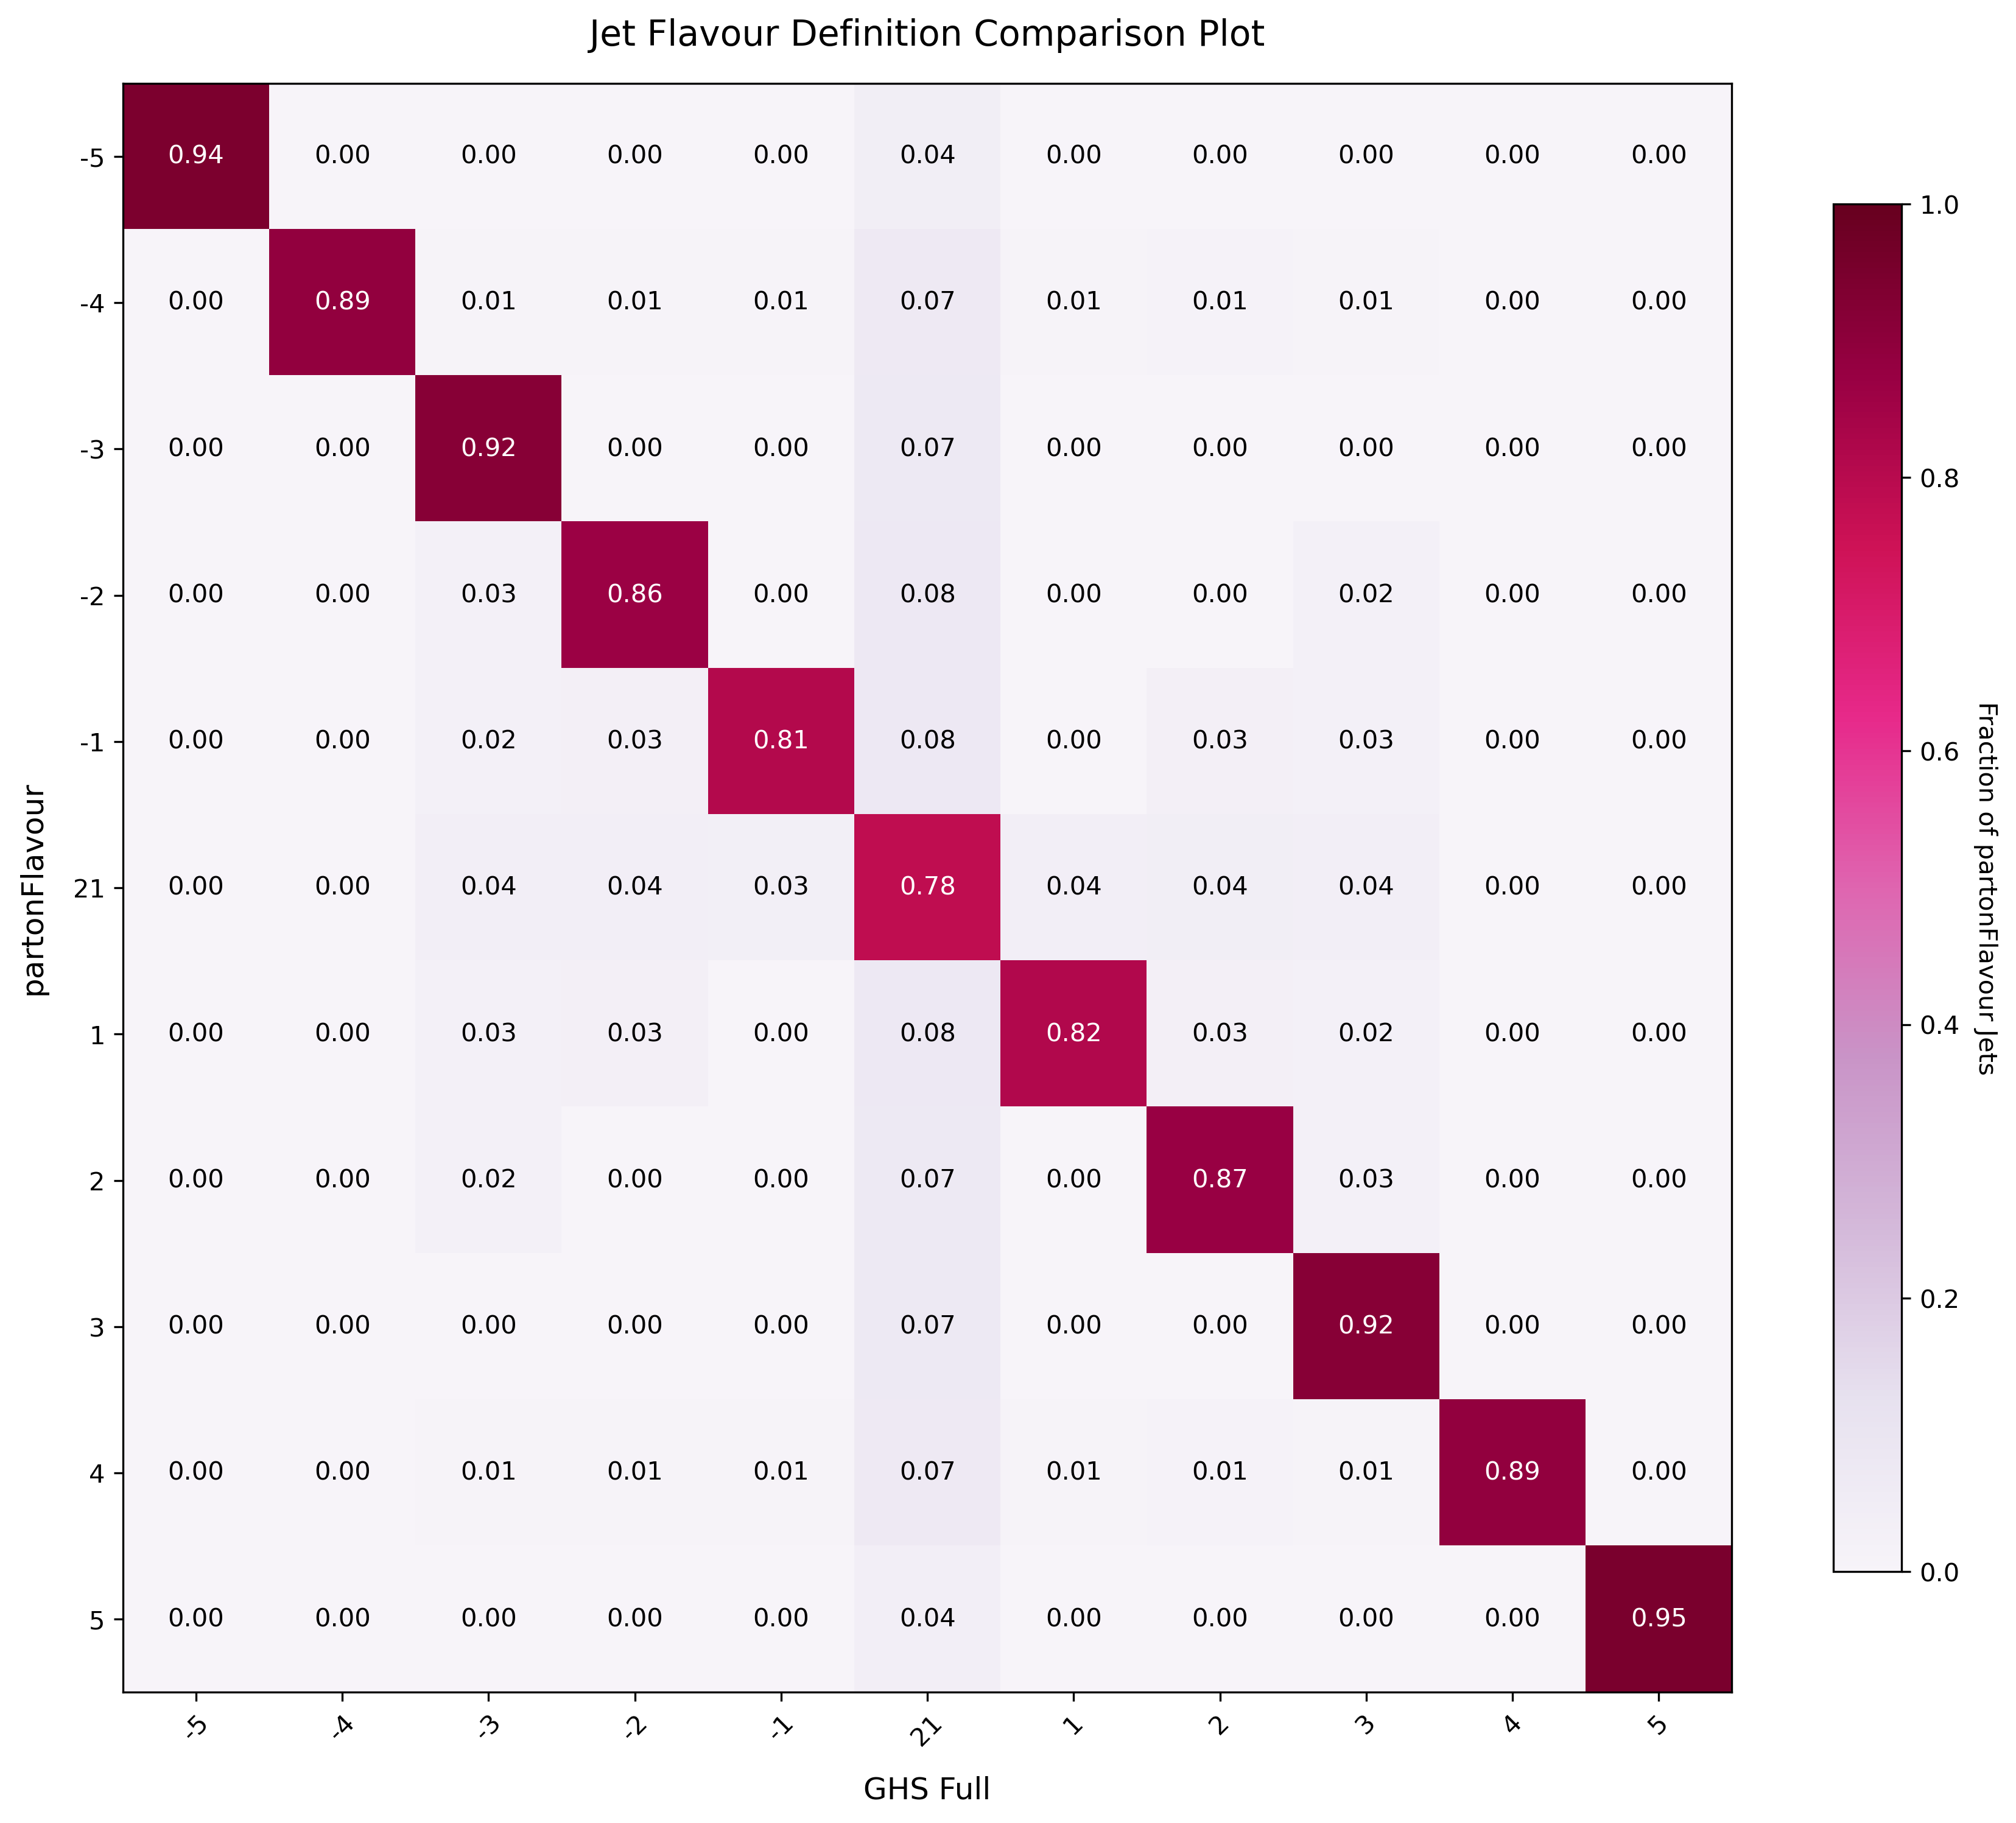
\includegraphics[width=0.56\textwidth]{images/compare_matrix_partonFlavour_vs_GHS_full_noLep.png}
    \caption{Jet flavour assignment matrix for full-chain simulated jets using the conventional $\parFlav$ definition (vertical axis) versus the GHS algorithm (horizontal axis). The heaviest flavour component of the GHS algorithm result is used for the comparison. The ratios are normalized to the total number of jets in each $\parFlav$ category, showing the agreement and differences between the two definitions.}
    \label{fig:reco_jet_compare_matrix_partonFlavour_vs_GHS_full_noLep}
\end{figure*}

\begin{figure*}[!bth]
    \centering
    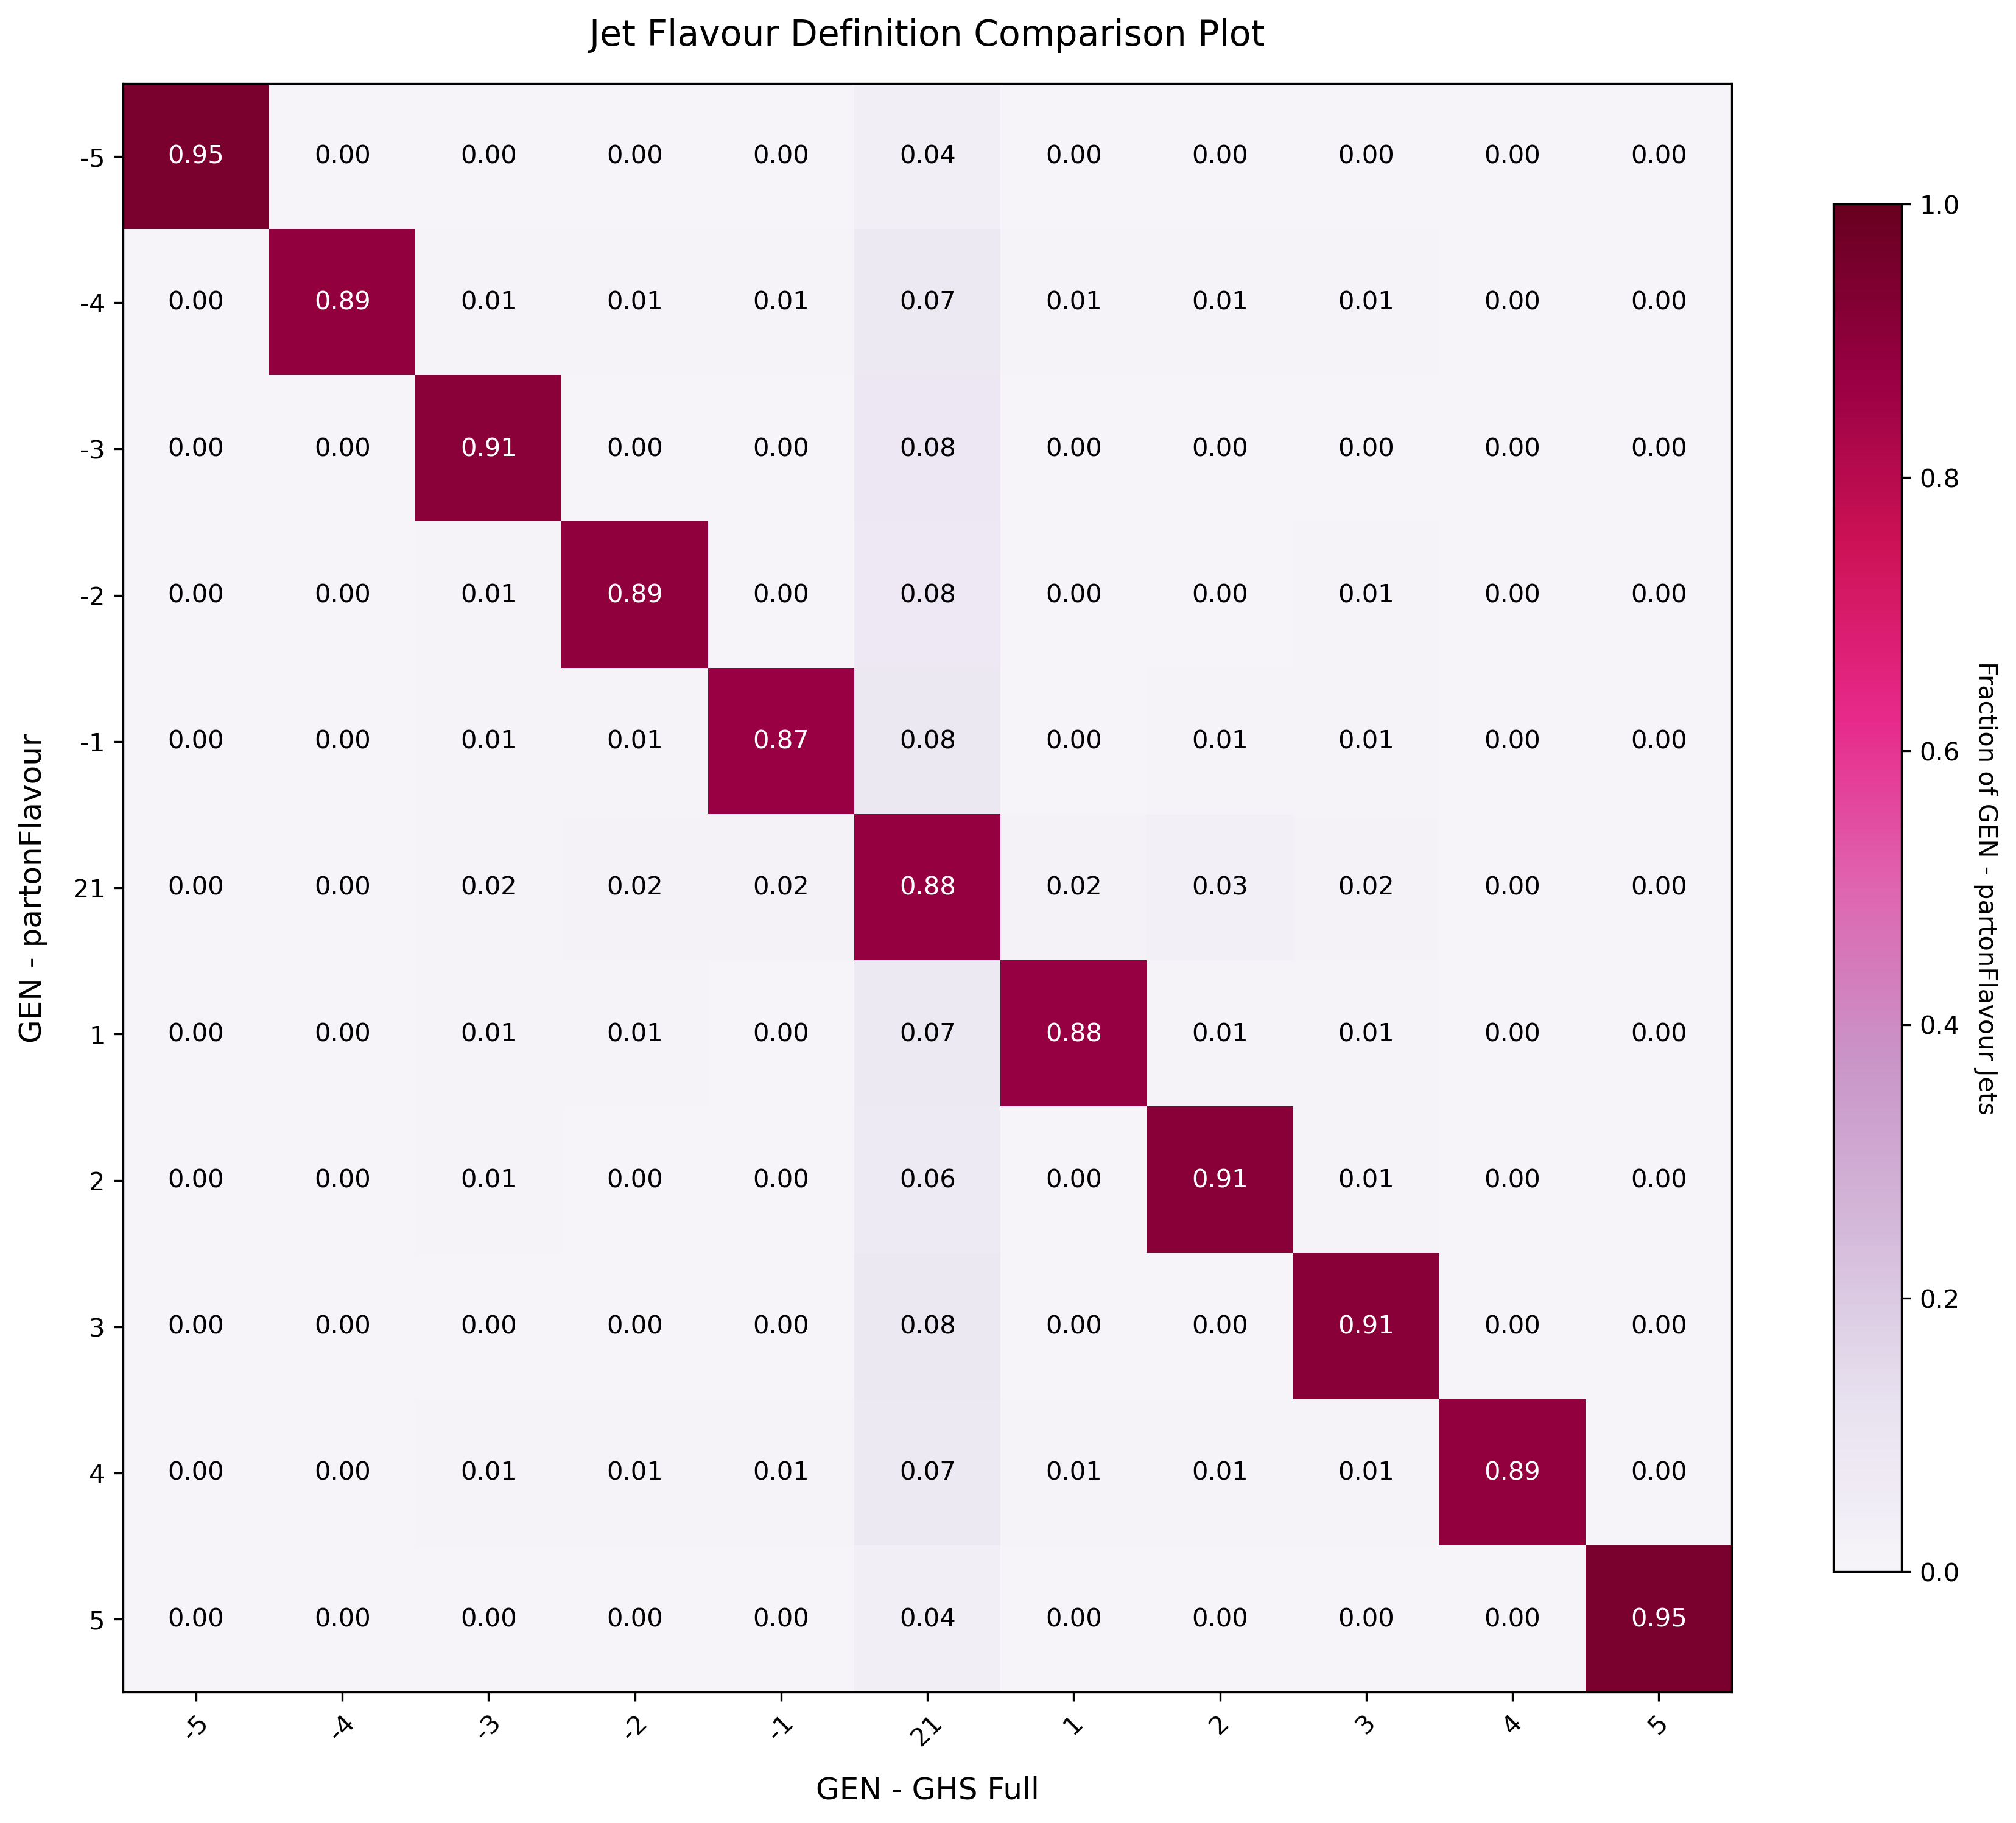
\includegraphics[width=0.56\textwidth]{images/compare_matrix_GenJet_partonFlavour_vs_GHS_full_noLep.png}
    \caption{Jet flavour assignment matrix for generator-level jets using the conventional $\parFlav$ definition (vertical axis) versus the GHS algorithm (horizontal axis). The heaviest flavour component of the GHS algorithm result is used for the comparison. The ratios are normalized to the total number of jets in each $\parFlav$ category, showing the agreement and differences between the two definitions.}
    \label{fig:gen_jet_compare_matrix_partonFlavour_vs_GHS_full_noLep}
\end{figure*}


\begin{figure*}[!htbp]
    \centering
    \begin{subfigure}[t]{0.48\textwidth}
        \centering
        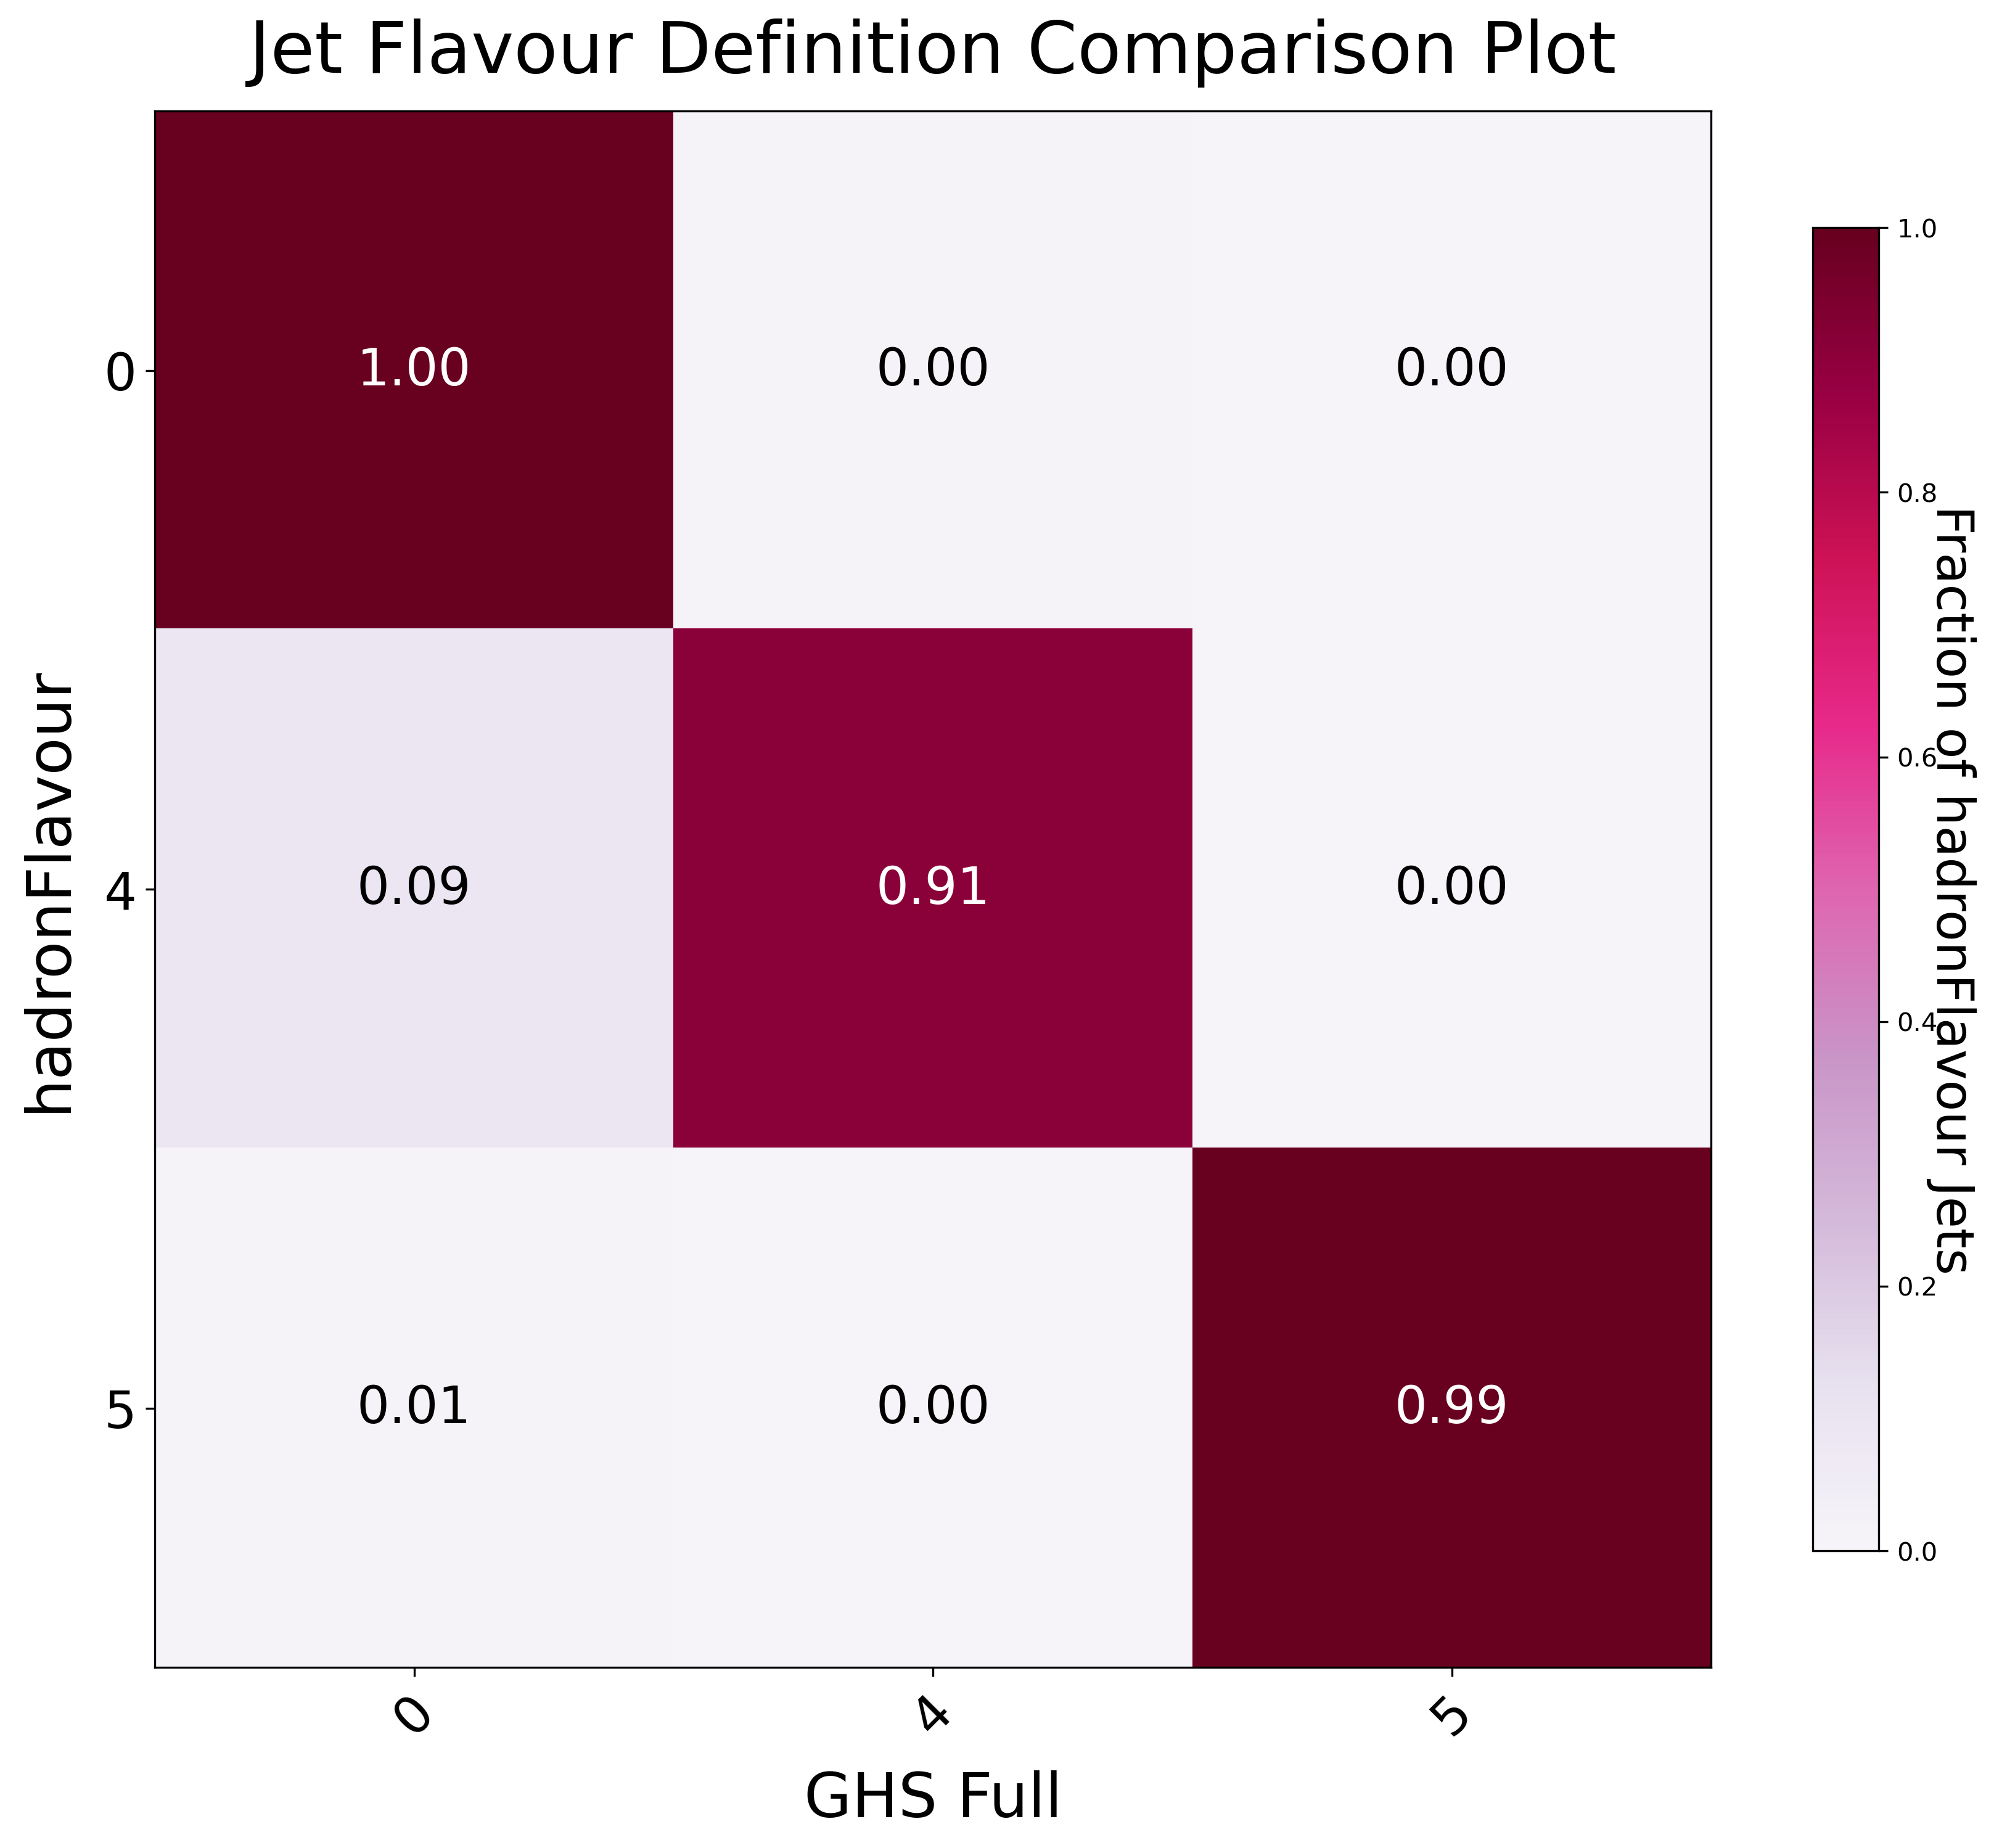
\includegraphics[width=\textwidth]{images/compare_matrix_hadronFlavour_vs_GHS_full.png}
        \caption{Full-chain simulated jets}
        \label{fig:reco_jet_compare_matrix_hadronFlavour_vs_GHS_full}
    \end{subfigure}
    \hfill
    \begin{subfigure}[t]{0.48\textwidth}
        \centering
        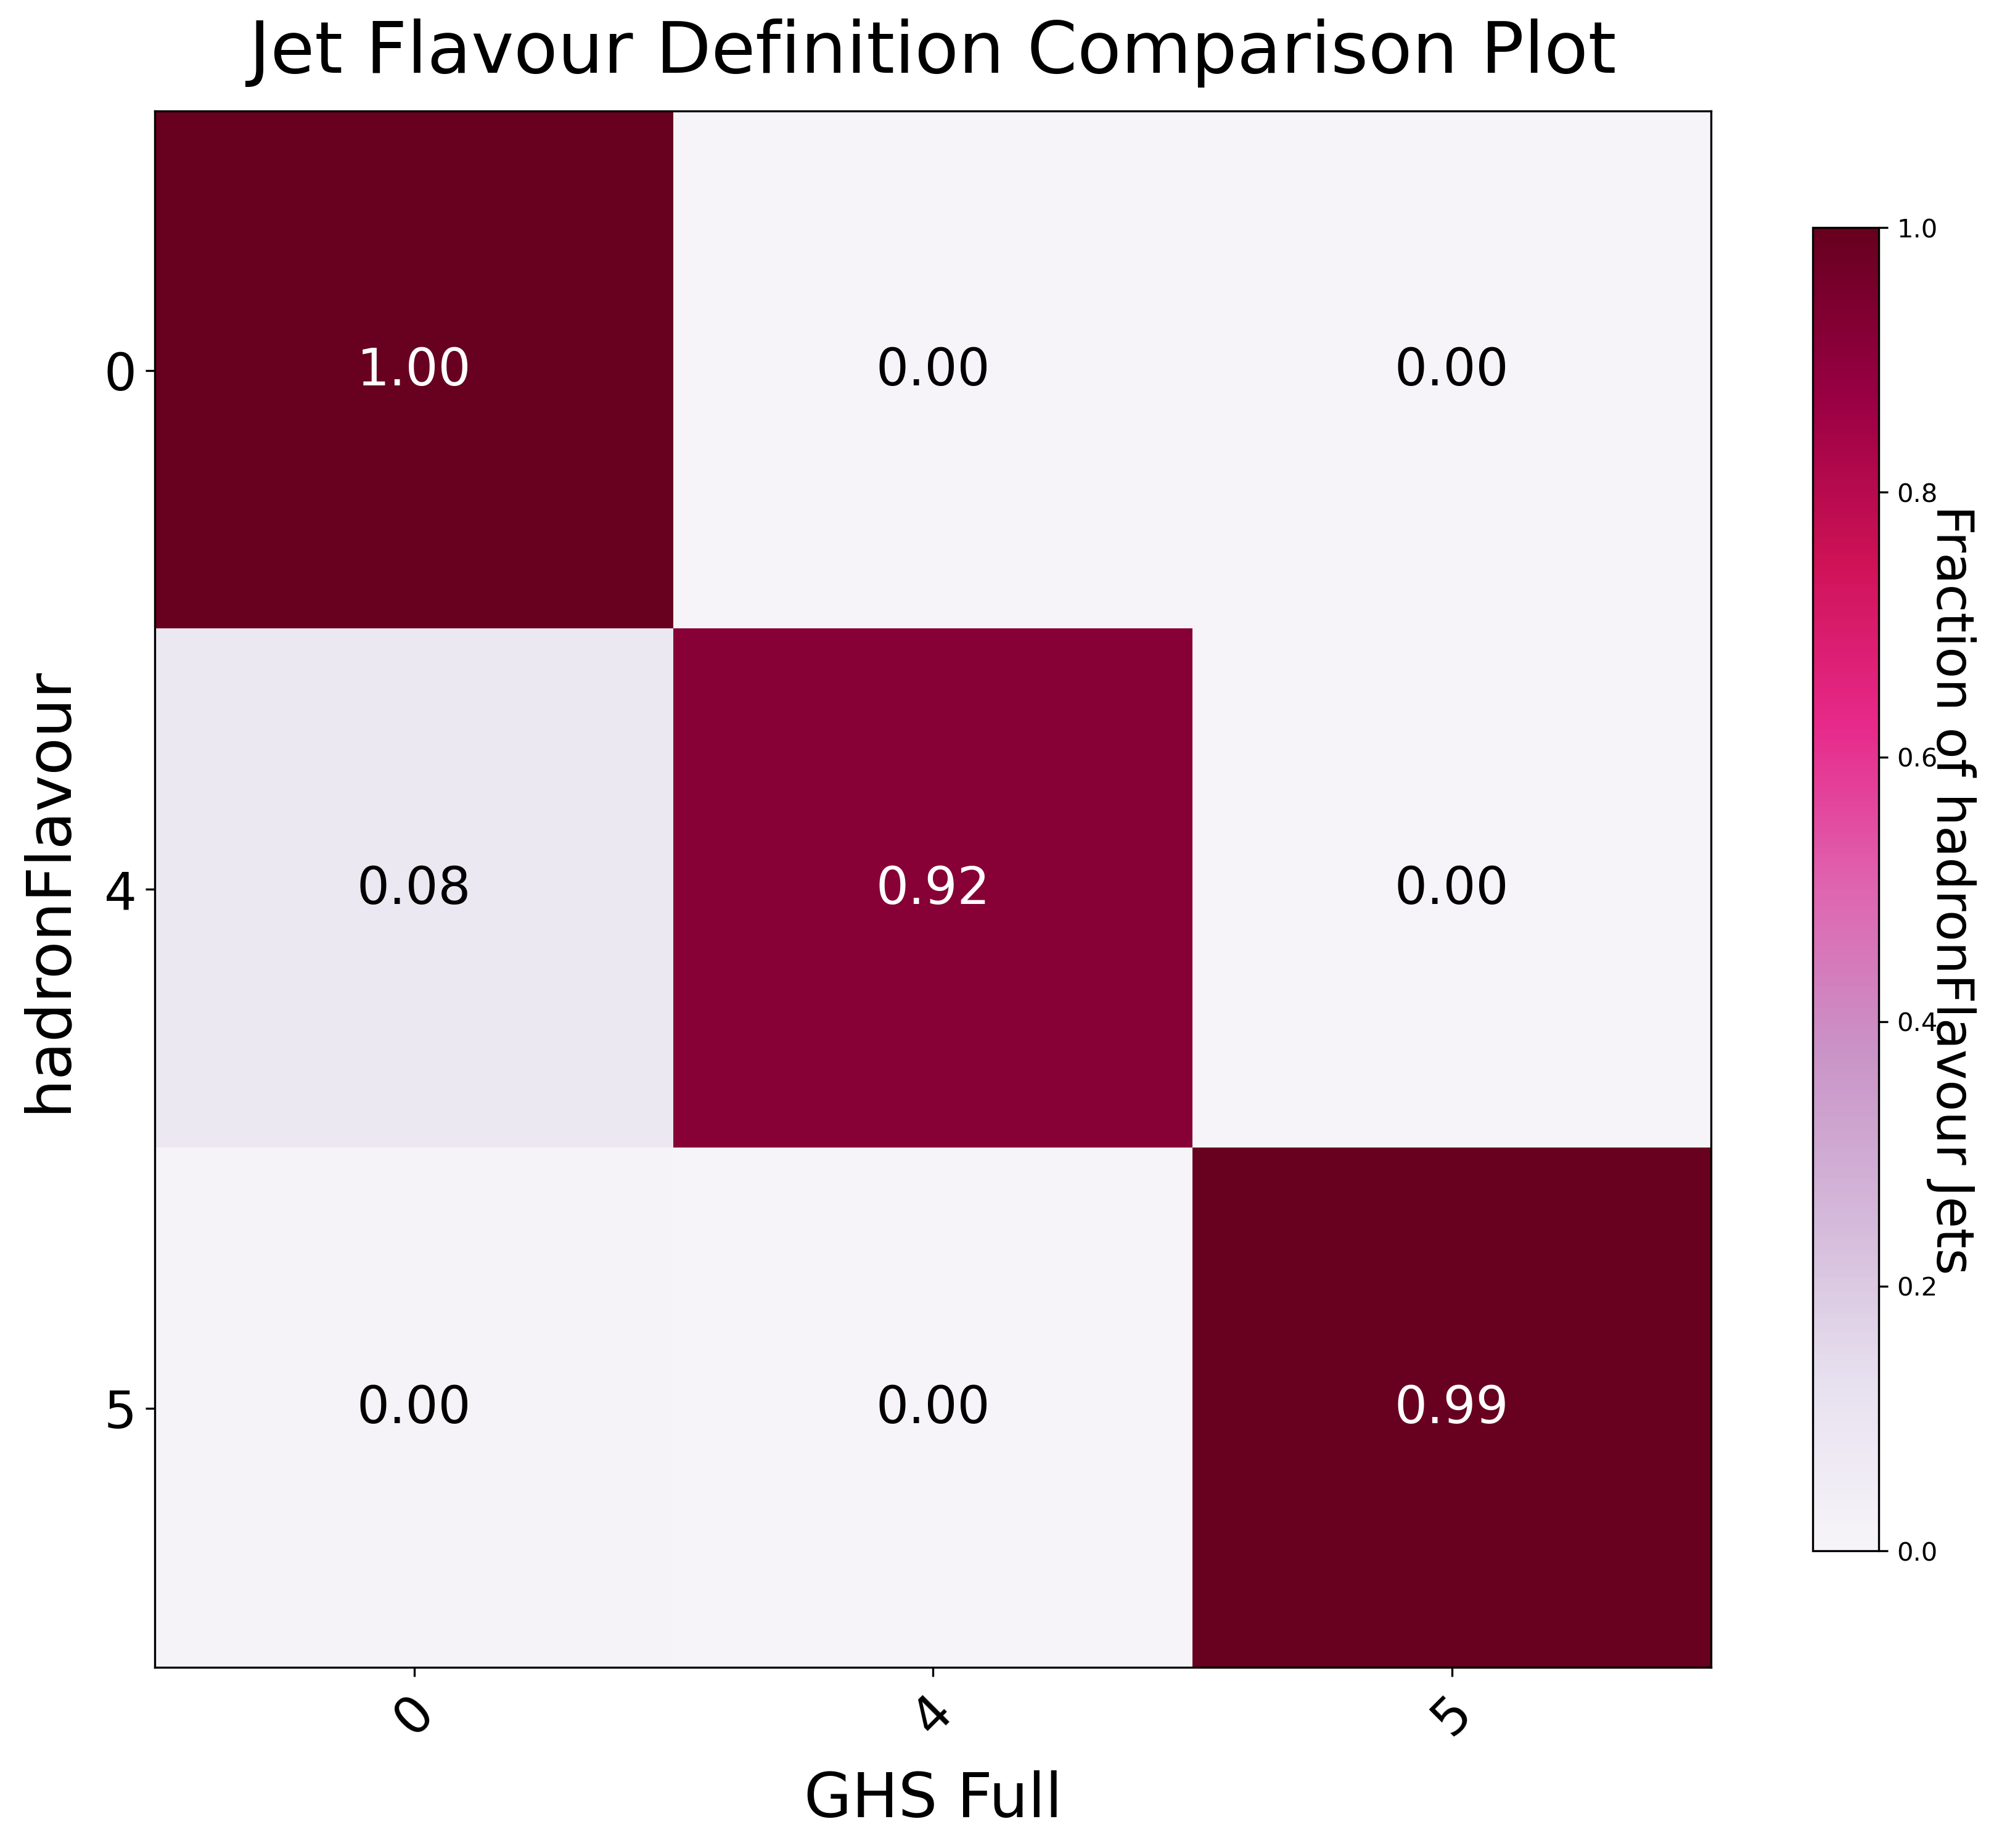
\includegraphics[width=\textwidth]{images/compare_matrix_GenJet_hadronFlavour_vs_GHS_full.png}
        \caption{Generator-level jets}
        \label{fig:gen_jet_compare_matrix_hadronFlavour_vs_GHS_full}
    \end{subfigure}
    \caption{Jet flavour assignment matrices using the conventional $\hadFlav$ definition (vertical axis) versus the GHS algorithm (horizontal axis). The heaviest flavour component of the GHS algorithm result is used for the comparison, with $q$ and $\bar{q}$ marked as the same flavour. The ratios are normalized to the total number of jets in each $\hadFlav$ category, showing the agreement and differences between the two definitions. (\subref{fig:reco_jet_compare_matrix_hadronFlavour_vs_GHS_full}) Full-chain simulated jets; (\subref{fig:gen_jet_compare_matrix_hadronFlavour_vs_GHS_full}) Generator-level jets.}
    \label{fig:compare_matrix_hadronFlavour_vs_GHS_full}
\end{figure*}

The $\parFlav$- or $\hadFlav$-defined heavy flavour jets that are not identified as such by the GHS algorithm are primarily reclassified as flavour-neutral jets, indicating a possible origin of light quarks or gluons. To further understand the nature of this special class of jets, we perform a detailed comparison of their kinematic and flavour-tagging characteristics in the following section, against those jets identified as heavy-flavour by both conventional and GHS algorithm definitions.

\subsection{Jet Characteristics Comparison} %[TODO]
\label{sec:vali-vars}

Two classes of jets are further compared: heavy-flavour jets by both definitions, and heavy-flavour jets by conventional definitions ("$\parFlav$" or "$\hadFlav$") but flavour-neutral by GHS. To demonstrate the origin of the two classes of jets, distributions of the following variables are compared:

\begin{itemize}
    \item Jet transverse momentum ($p_T$): genuine heavy-flavour jets are expected to have a harder $p_T$ spectrum due to the larger mass of the initiating quark;
    \item Number of associated heavy-flavour hadrons ("$\texttt{nBHadrons}$" or "$\texttt{nCHadrons}$" for b- and c- jets, respectively): such variables are derived from the ghost clustering association process for $\hadFlav$ definition for generator-level jets; despite being IRC-unsafe variables, they provide insight into the partonic origin of the jets;
    \item Number of secondary vertices (SVs) within the jets ($\texttt{nSVs}$): in reconstructed jets, the flavour information of a hadron is not directly accessible, yet given the relatively long lifetimes of b- and c-hadrons, the presence of SVs within a jet may serve as a strong indicator of heavy-flavour origin, and the properties of SVs are widely used in flavour tagging algorithms;
    \item Flavour tagging scores from \textsc{ParticleNet} \cite{quParticleNetJetTagging2020} and \textsc{ParticleTransformer} \cite{quParticleTransformerJet2024} (only for reconstructed b-jets): \textsc{ParticleNet} and \textsc{ParticleTransformer} represent the state-of-the-art in machine learning-based flavour tagging algorithms at CMS. In CMS workflows, such algorithms are trained on jets labelled by the conventional $\hadFlav$, yet they are expected to learn the underlying physics and thus should also be effective in identifying genuine heavy-flavour jets. Comparing the flavour tagging scores between the two classes of jets provides a practical perspective on their flavour nature.
\end{itemize}

\subsubsection{Jet Transverse Momentum (\texorpdfstring{$p_T$}{pT})}
\label{sec:vali-vars-pt}

\begin{figure*}[!htbp]
    \centering
    \begin{subfigure}[t]{0.48\textwidth}
        \centering
        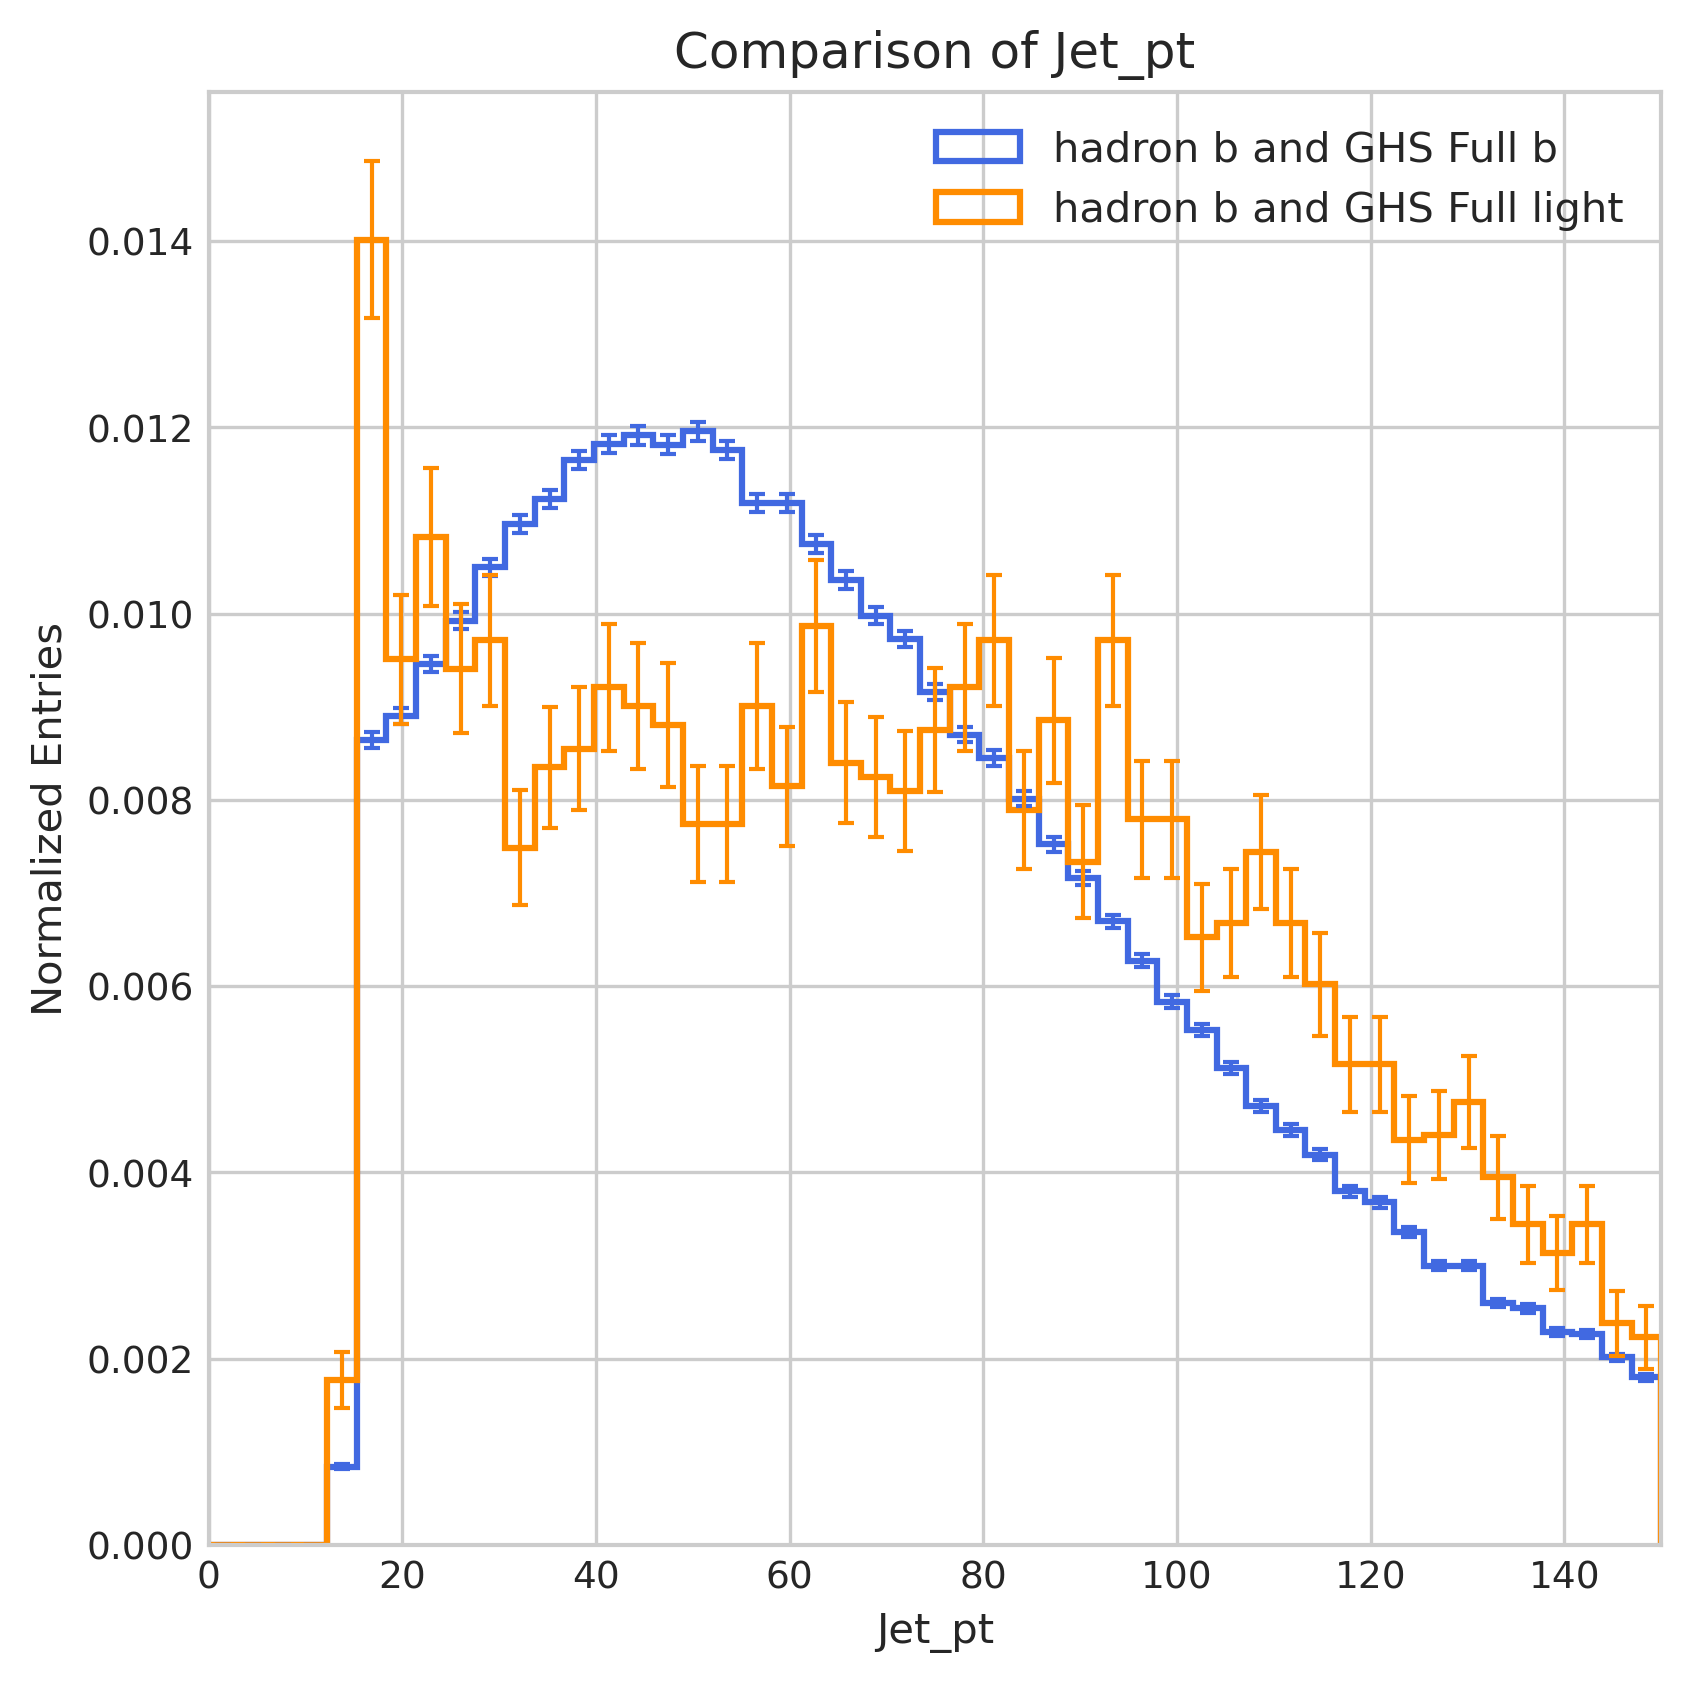
\includegraphics[width=\textwidth]{images/compare_pt_GHSFull_light_vs_b_filter_hadronFlavour_5.png}
        \caption{Full-chain simulated b-jets}
        \label{fig:pt_b_hadron_full}
    \end{subfigure}
    \hfill
    \begin{subfigure}[t]{0.48\textwidth}
        \centering
        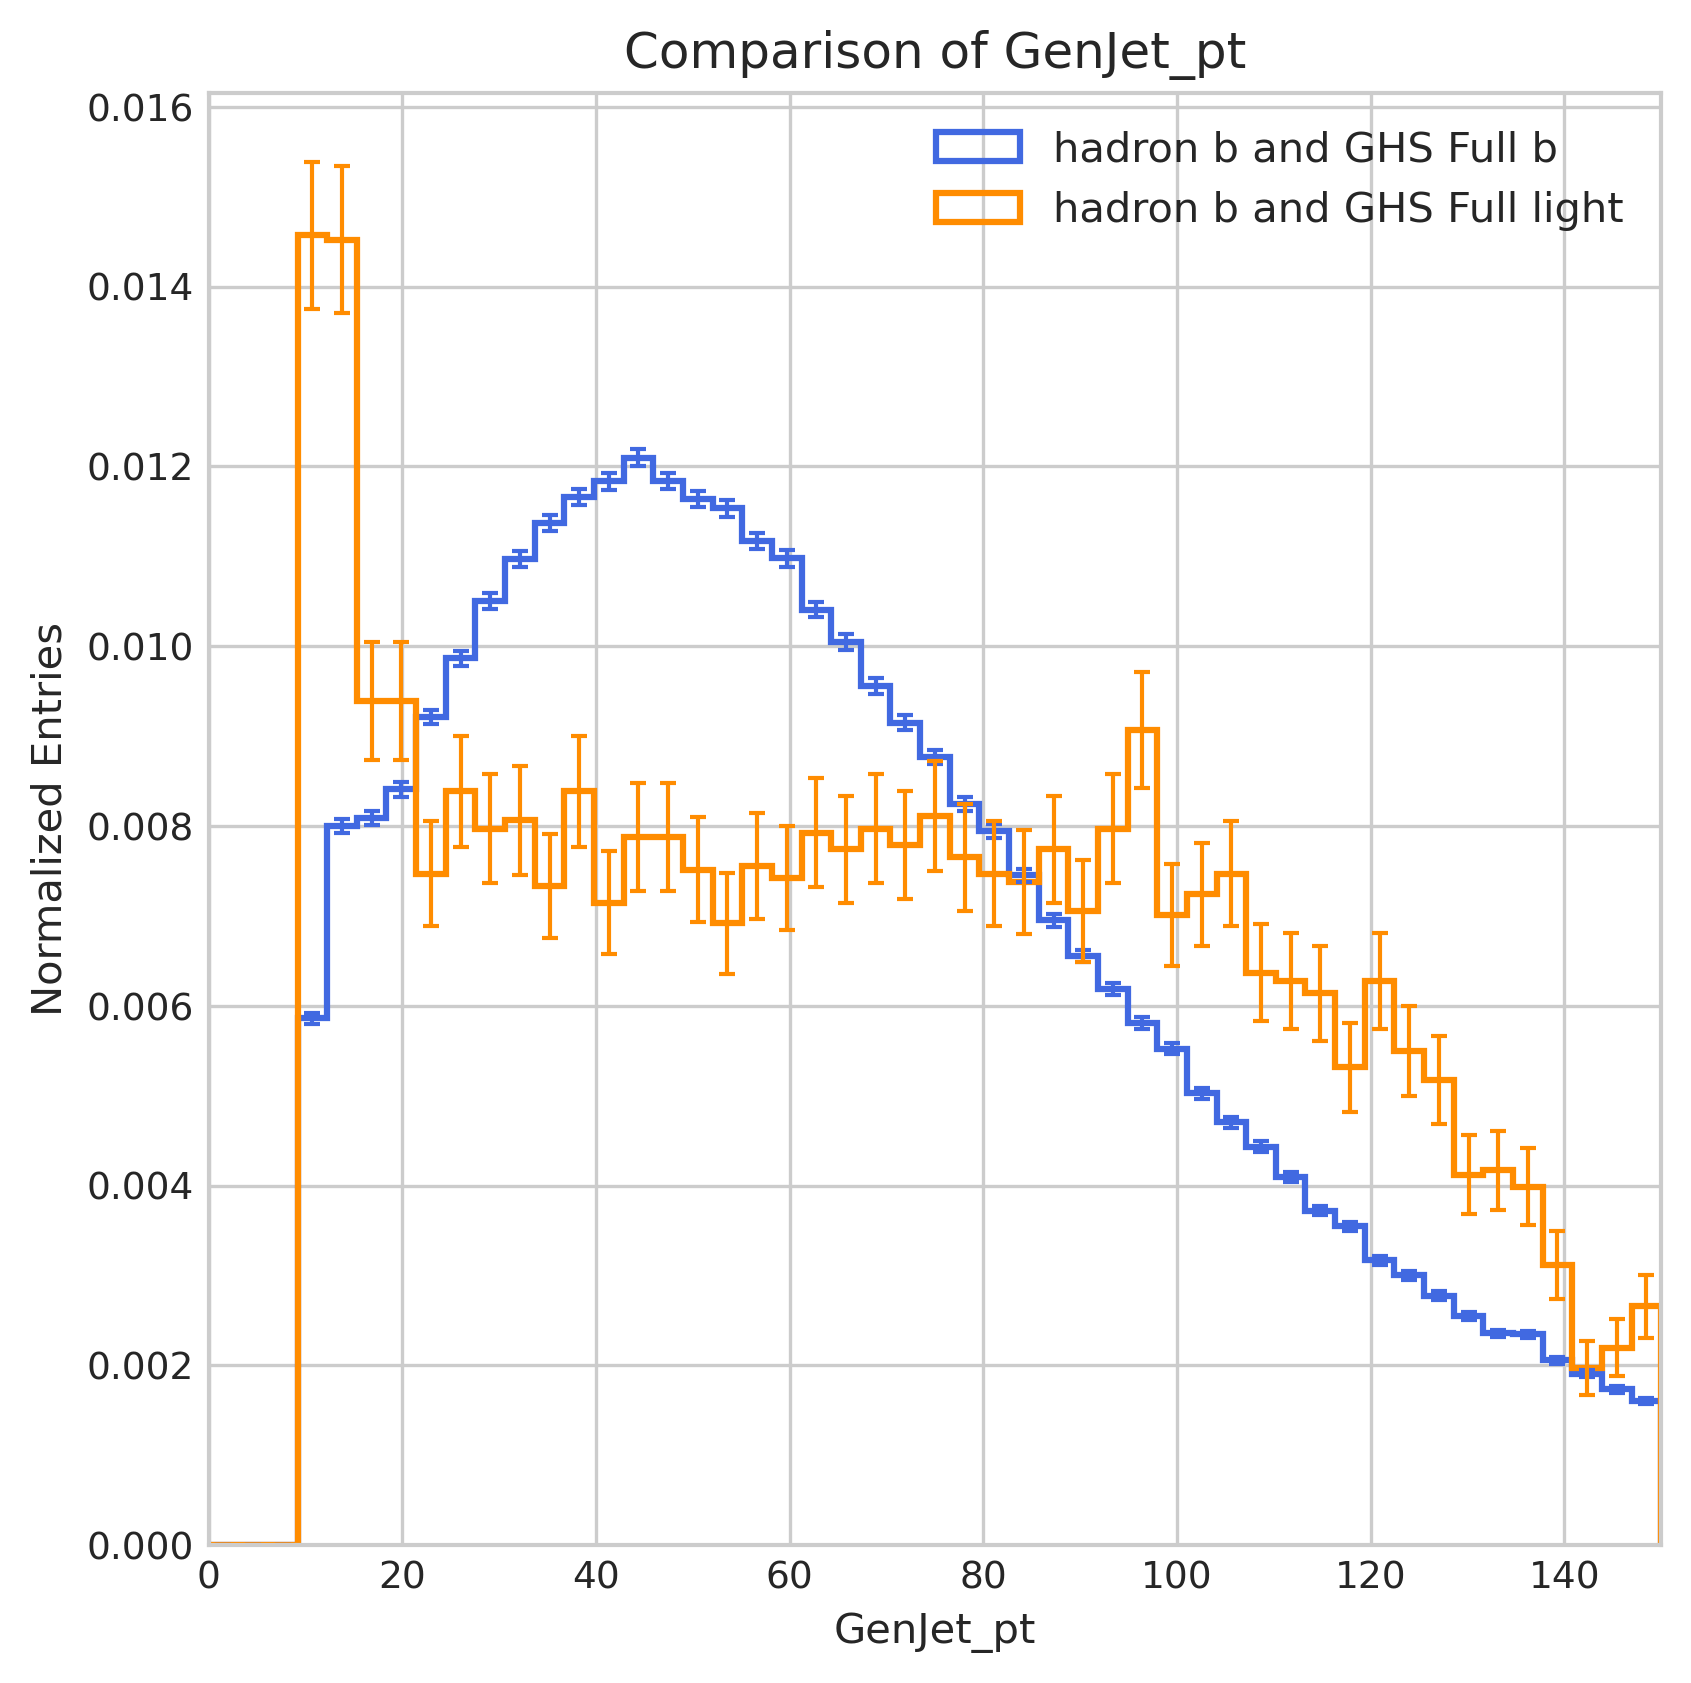
\includegraphics[width=\textwidth]{images/compare_GenJet_pt_GHSFull_light_vs_b_filter_hadronFlavour_5.png}
        \caption{Generator-level b-jets}
        \label{fig:pt_b_hadron_gen}
    \end{subfigure}
    \caption{Distributions of transverse momentum ($p_T$) for jets identified as b-jets by the $\hadFlav$ definition. The comparison is between two categories: jets also identified as b-flavour by the GHS algorithm (blue) and those classified as light-flavour by GHS (orange). The distributions are normalized to unit area for shape comparison. (\subref{fig:pt_b_hadron_full}) Full-chain simulation; (\subref{fig:pt_b_hadron_gen}) Generator-level.}
    \label{fig:pt_b_hadron_combined}
\end{figure*}

\begin{figure*}[!htbp]
    \centering
    \begin{subfigure}[t]{0.48\textwidth}
        \centering
        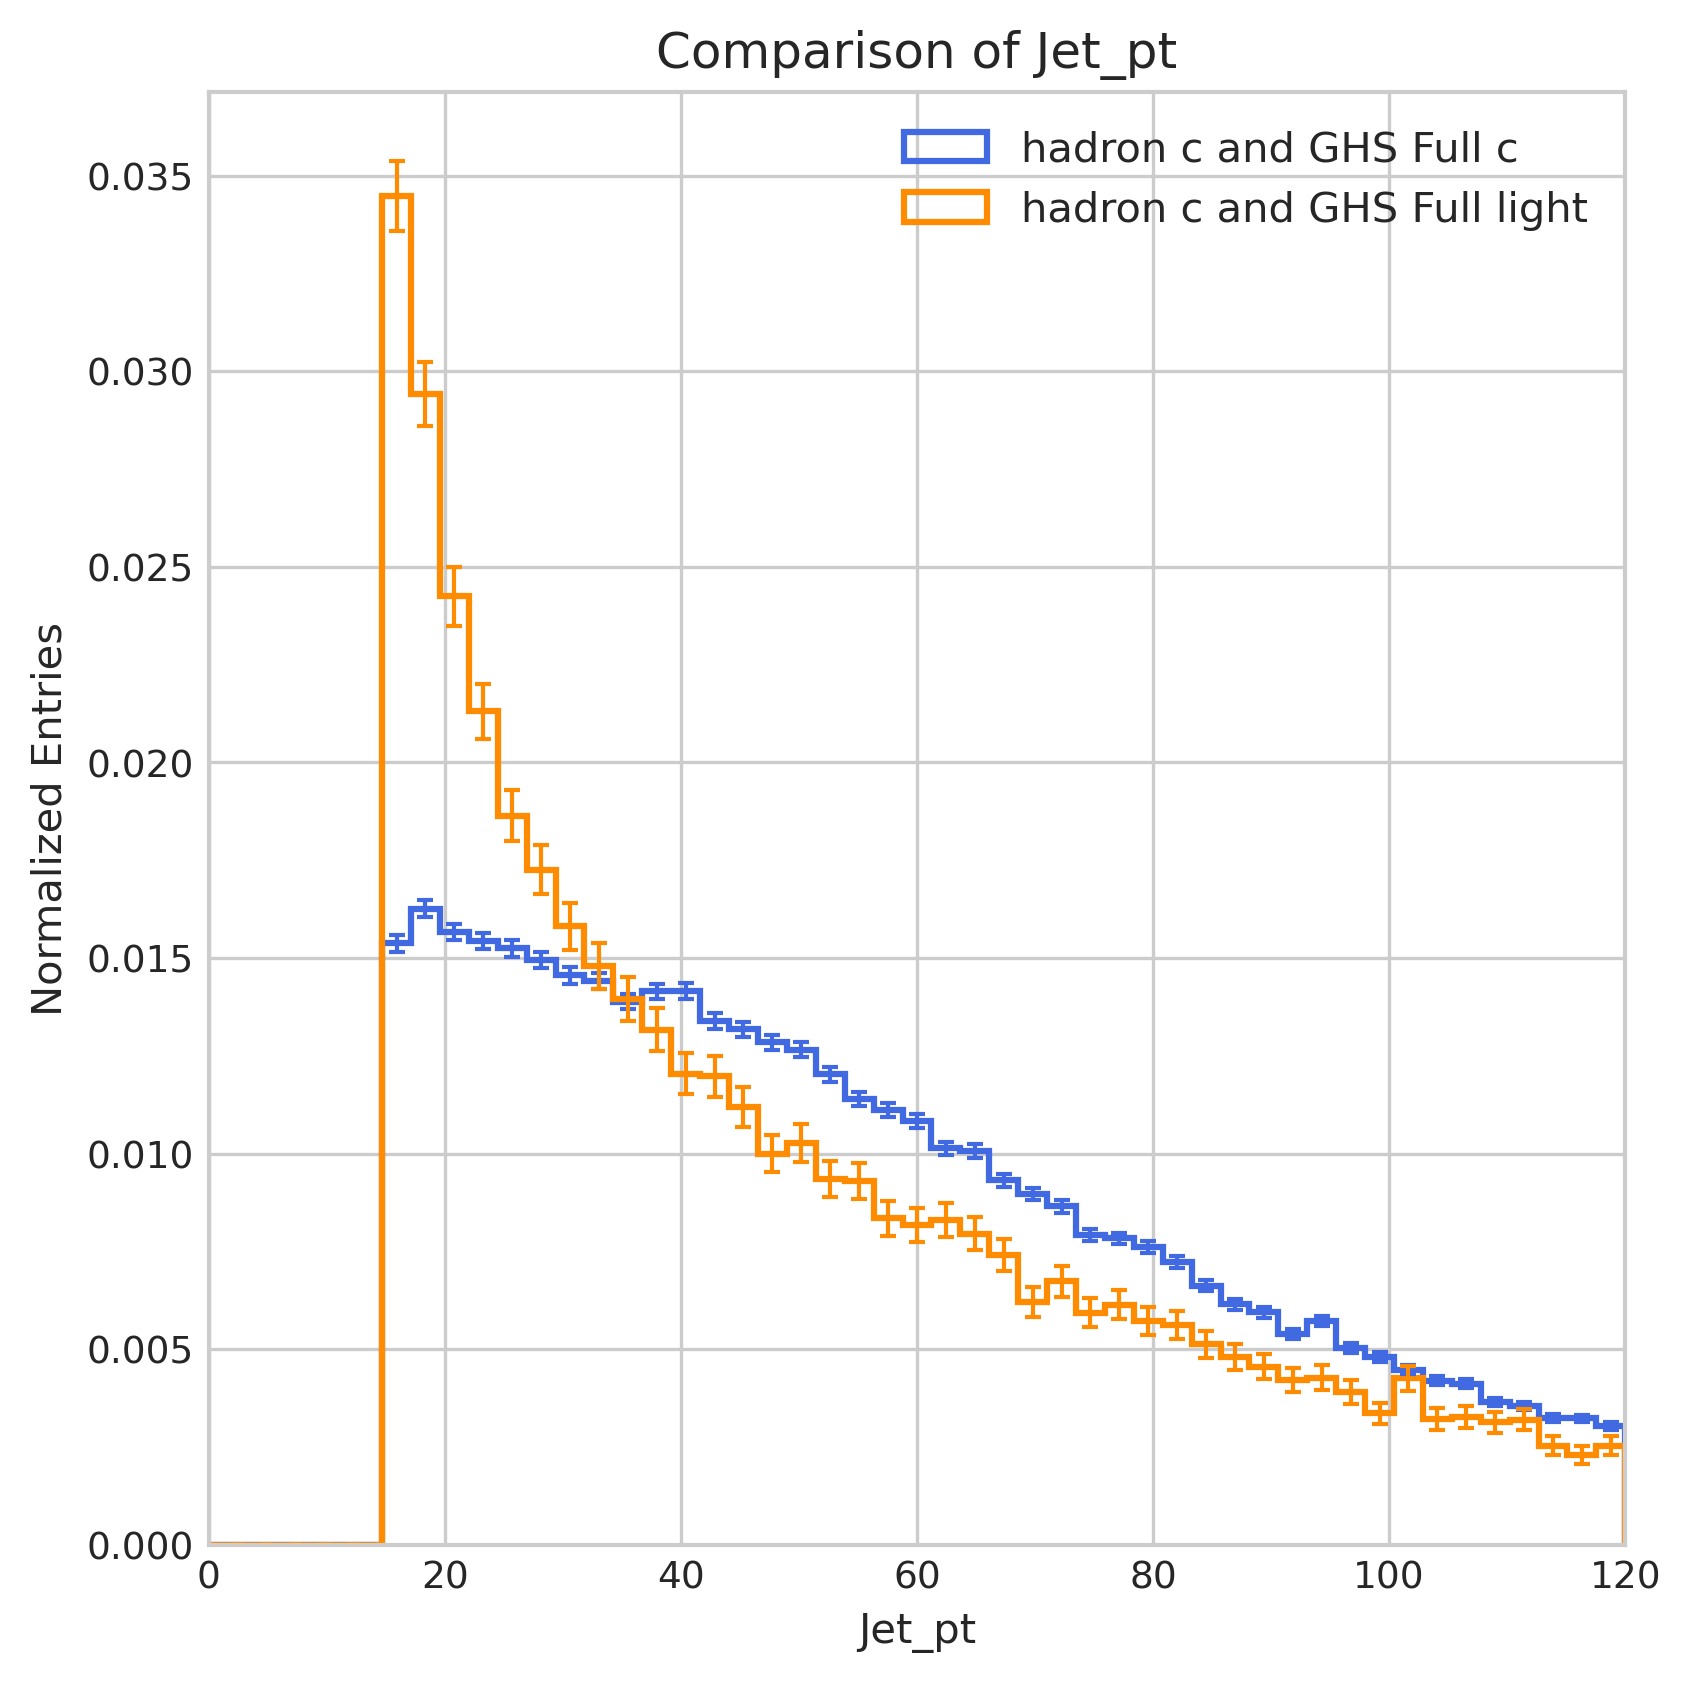
\includegraphics[width=\textwidth]{images/compare_pt_GHSFull_light_vs_c_filter_hadronFlavour_4.png}
        \caption{Full-chain simulated c-jets}
        \label{fig:pt_c_hadron_full}
    \end{subfigure}
    \hfill
    \begin{subfigure}[t]{0.48\textwidth}
        \centering
        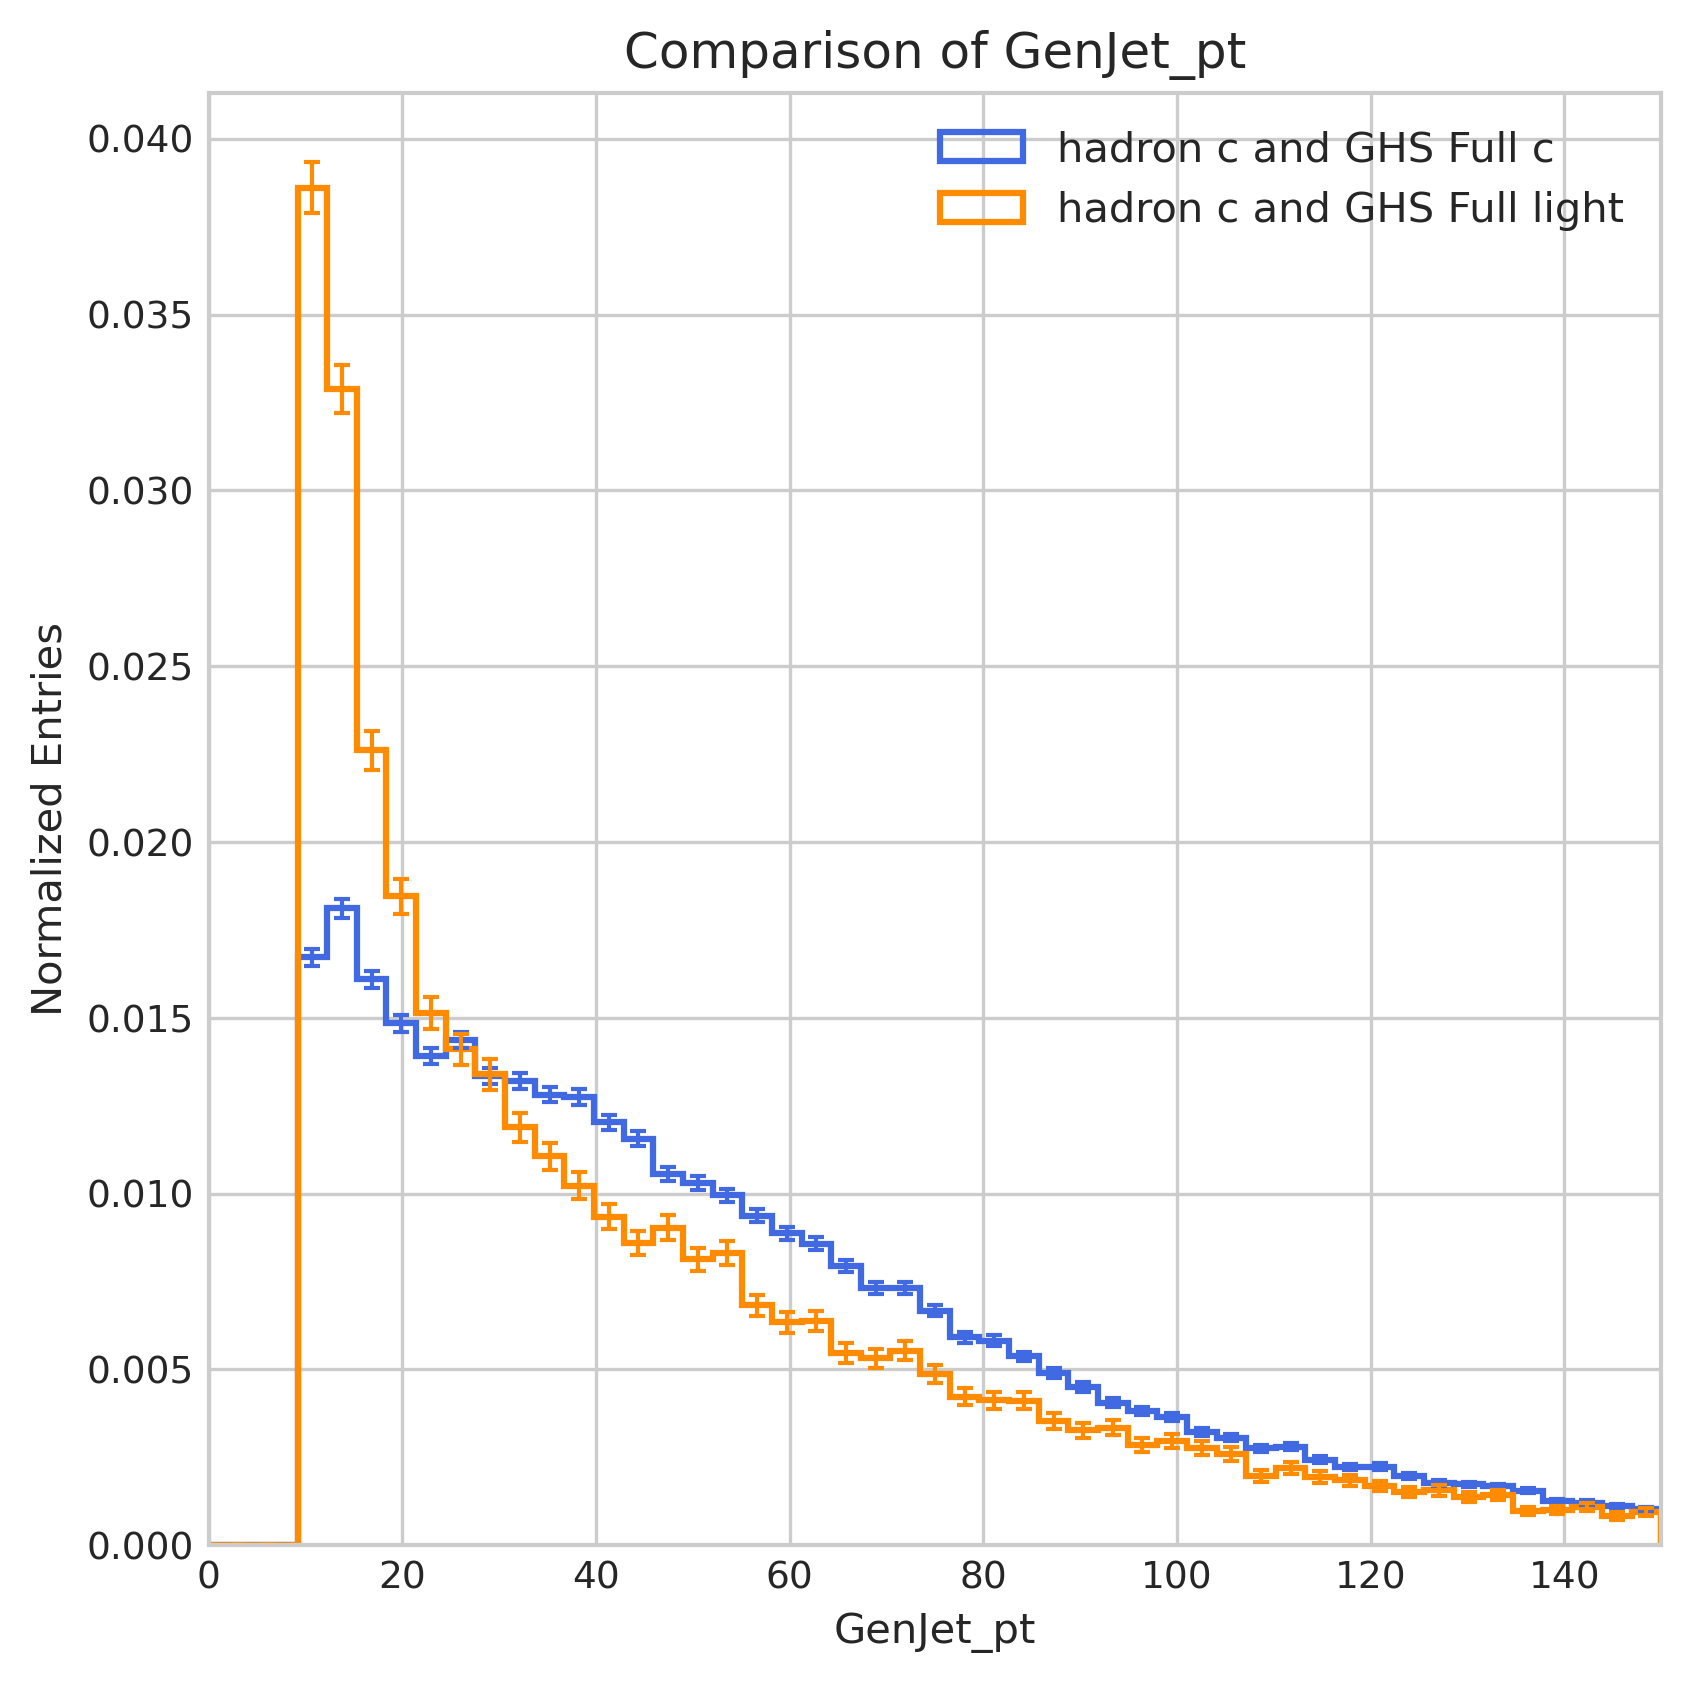
\includegraphics[width=\textwidth]{images/compare_GenJet_pt_GHSFull_light_vs_c_filter_hadronFlavour_4.png}
        \caption{Generator-level c-jets}
        \label{fig:pt_c_hadron_gen}
    \end{subfigure}
    \caption{Distributions of transverse momentum ($p_T$) for jets identified as c-jets by the $\hadFlav$ definition. The comparison is between two categories: jets also identified as c-flavour by the GHS algorithm (blue) and those classified as light-flavour by GHS (orange). The distributions are normalized to unit area for shape comparison. (\subref{fig:pt_c_hadron_full}) Full-chain simulation; (\subref{fig:pt_c_hadron_gen}) Generator-level.}
    \label{fig:pt_c_hadron_combined}
\end{figure*}

\begin{figure*}[!htbp]
    \centering
    \begin{subfigure}[t]{0.48\textwidth}
        \centering
        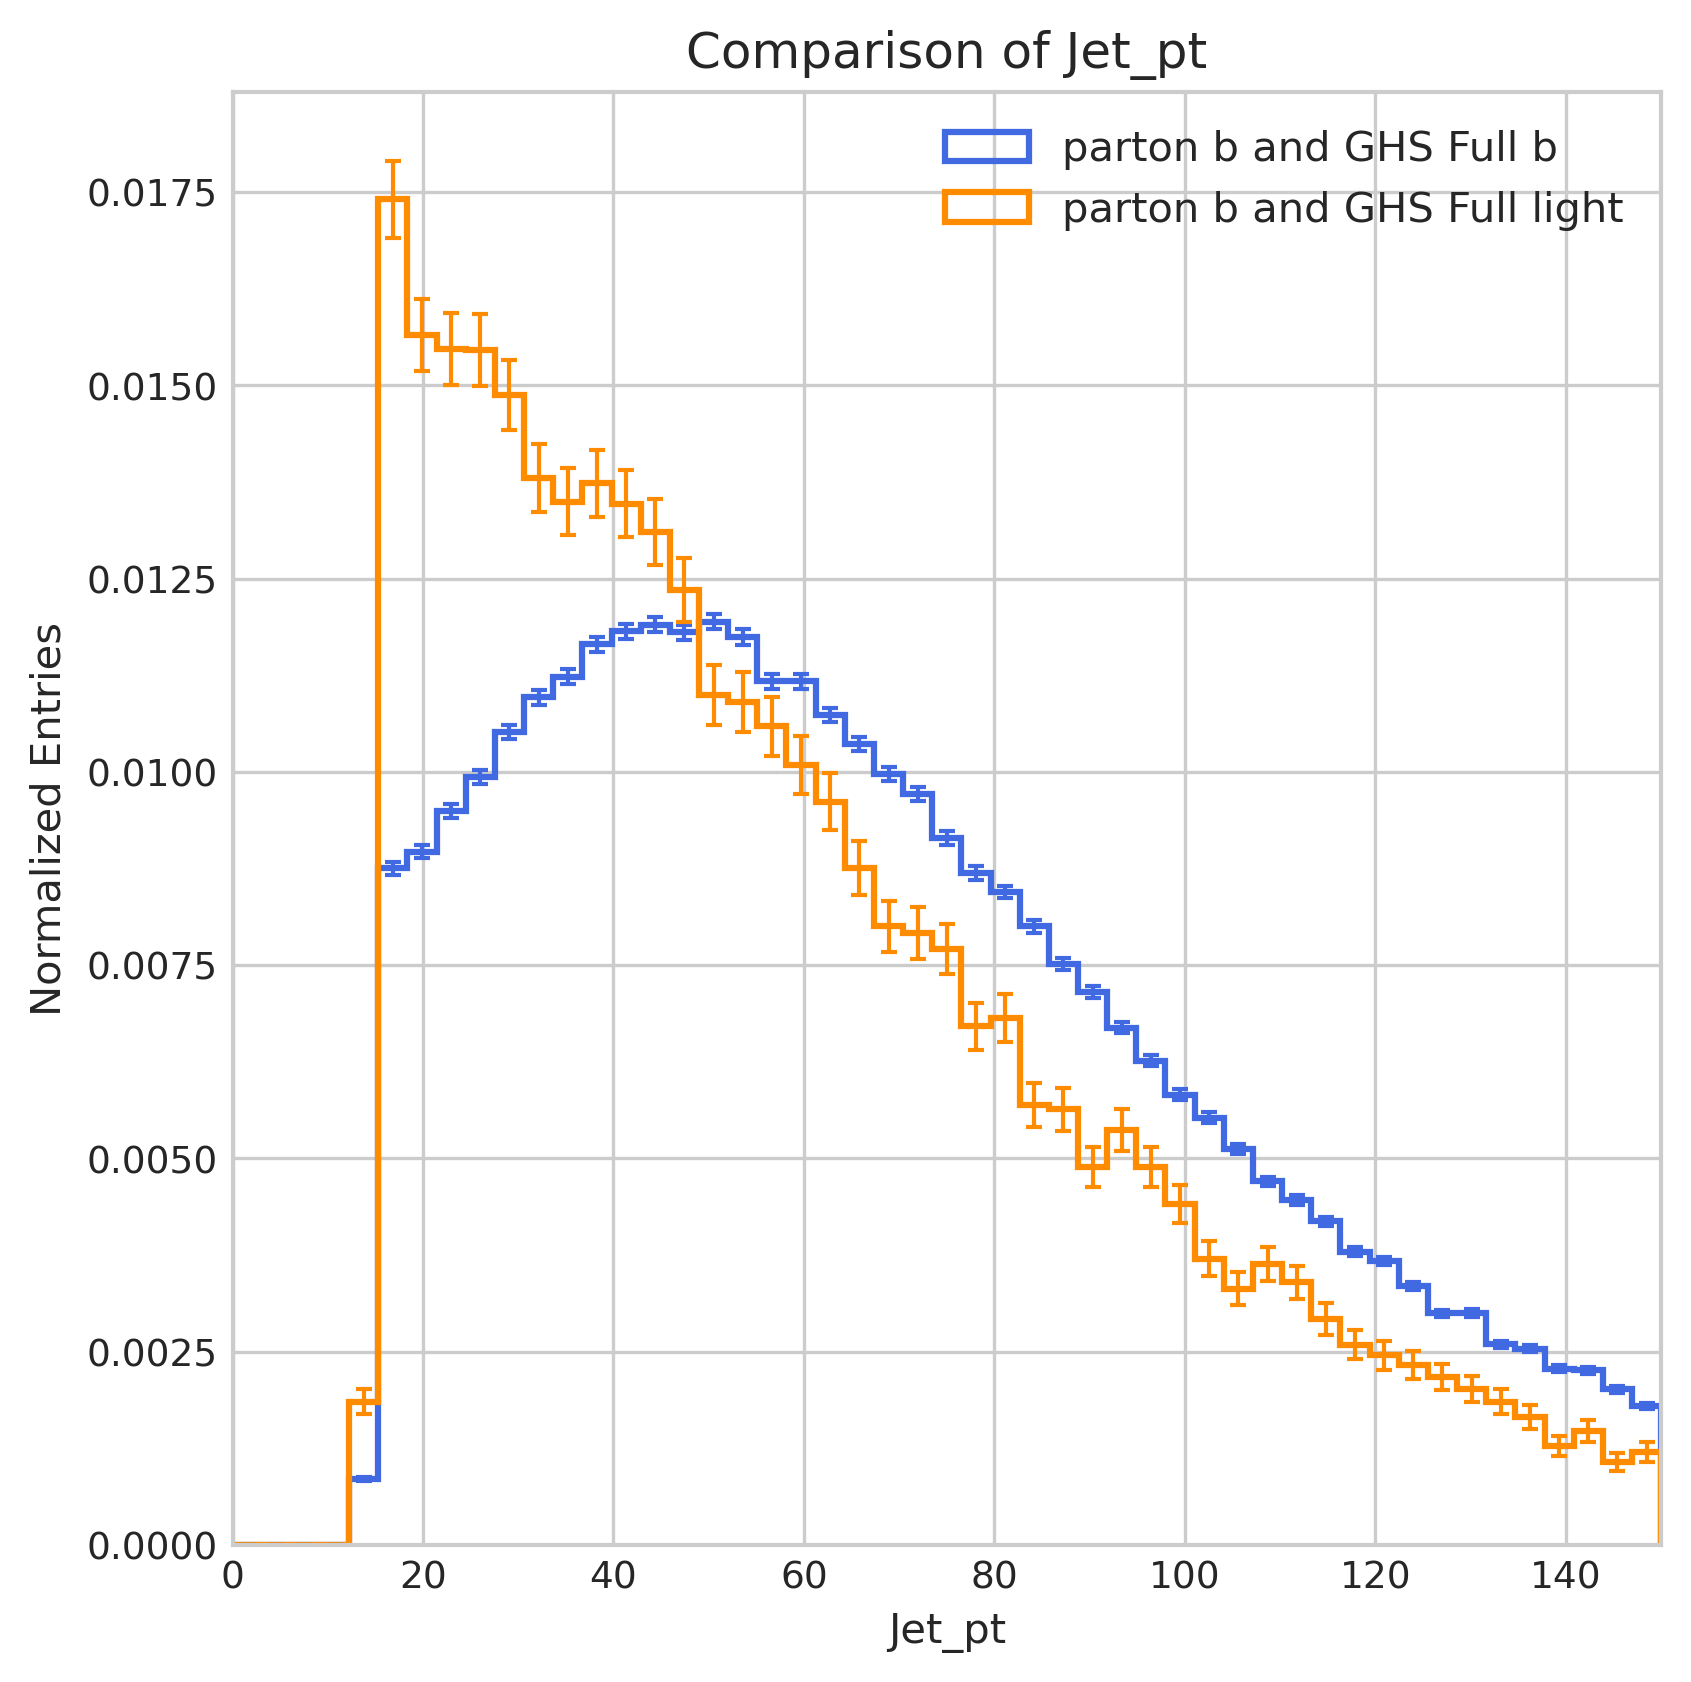
\includegraphics[width=\textwidth]{images/compare_pt_GHSFull_light_vs_b_filter_partonFlavour_5.png}
        \caption{Full-chain simulated b-jets}
        \label{fig:pt_b_parton_full}
    \end{subfigure}
    \hfill
    \begin{subfigure}[t]{0.48\textwidth}
        \centering
        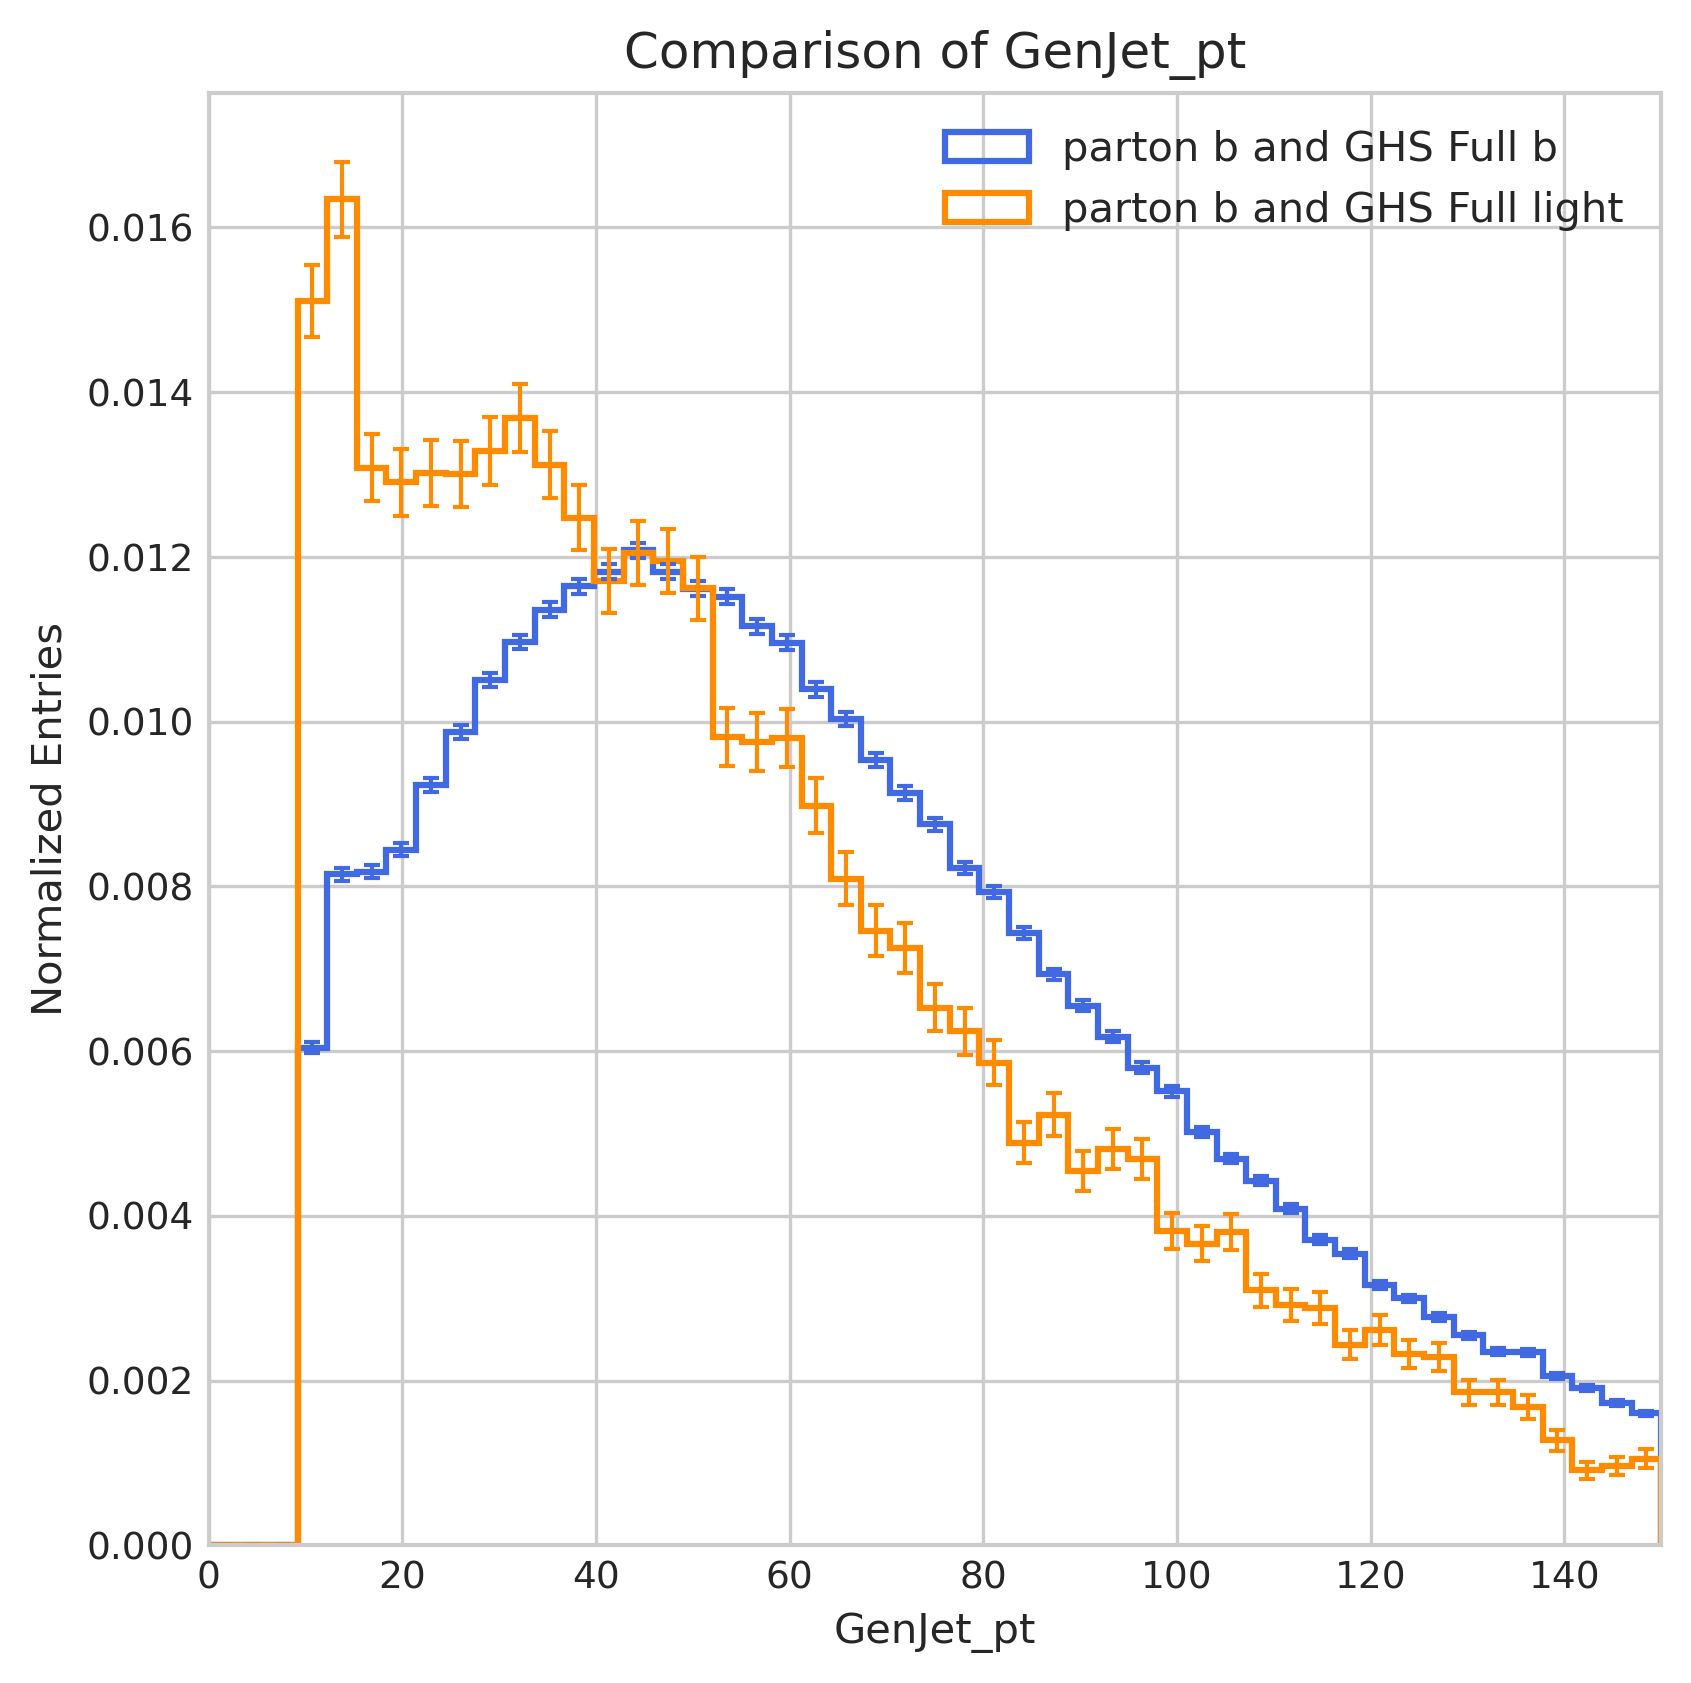
\includegraphics[width=\textwidth]{images/compare_GenJet_pt_GHSFull_light_vs_b_filter_partonFlavour_5.png}
        \caption{Generator-level b-jets}
        \label{fig:pt_b_parton_gen}
    \end{subfigure}
    \caption{Distributions of transverse momentum ($p_T$) for jets identified as b-jets by the $\parFlav$ definition. The comparison is between two categories: jets also identified as b-flavour by the GHS algorithm (blue) and those classified as light-flavour by GHS (orange). The distributions are normalized to unit area for shape comparison. (\subref{fig:pt_b_parton_full}) Full-chain simulation; (\subref{fig:pt_b_parton_gen}) Generator-level.}
    \label{fig:pt_b_parton_combined}
\end{figure*}

\begin{figure*}[!htbp]
    \centering
    \begin{subfigure}[t]{0.48\textwidth}
        \centering
        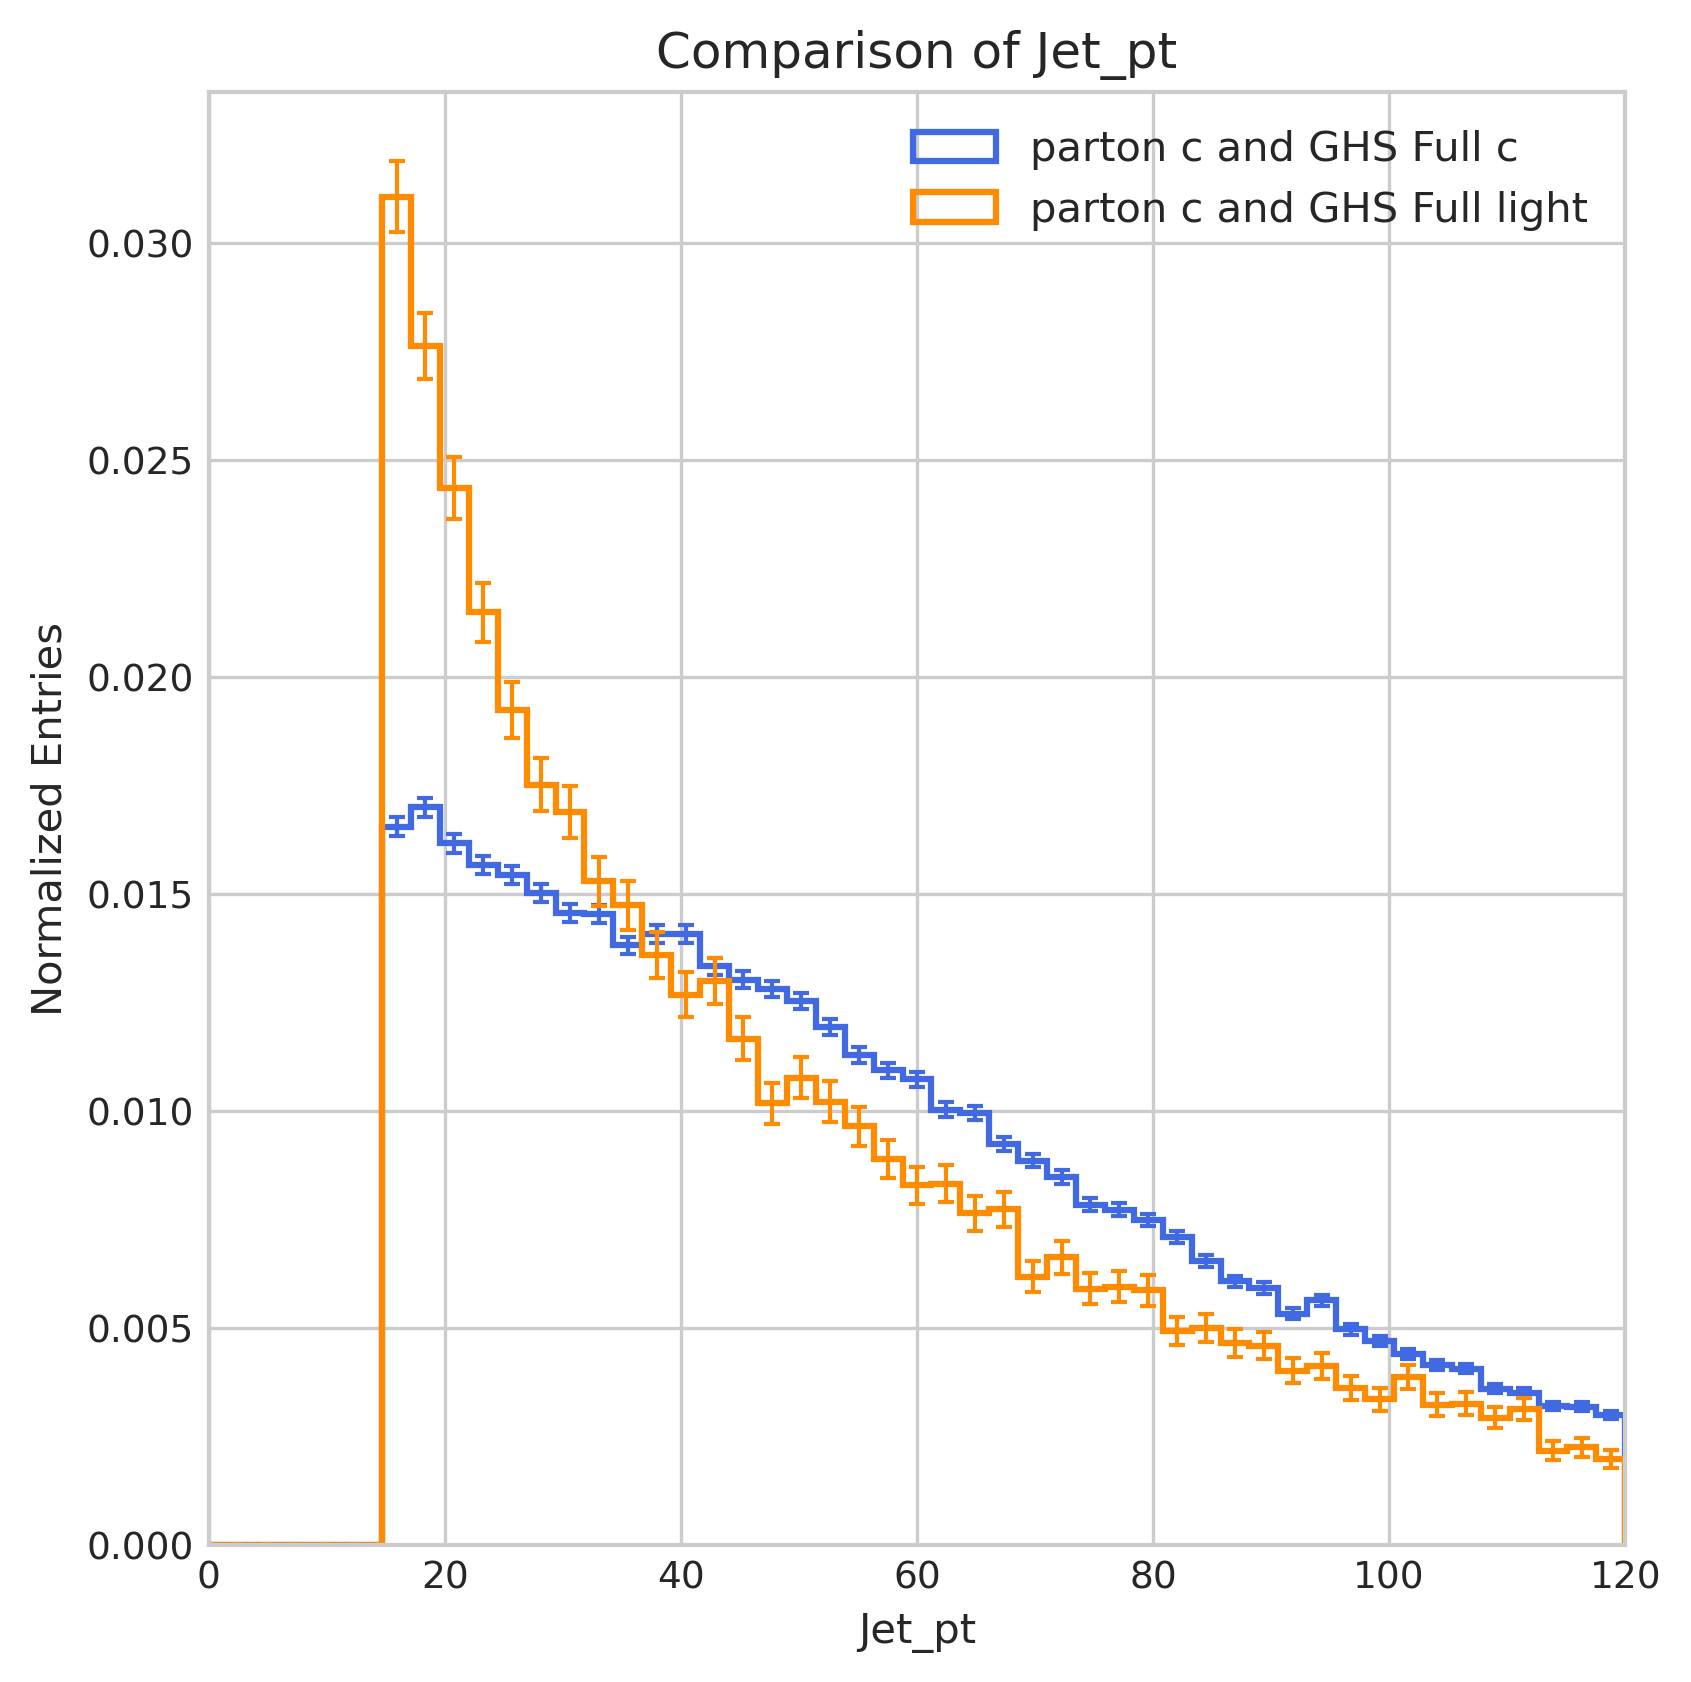
\includegraphics[width=\textwidth]{images/compare_pt_GHSFull_light_vs_c_filter_partonFlavour_4.png}
        \caption{Full-chain simulated c-jets}
        \label{fig:pt_c_parton_full}
    \end{subfigure}
    \hfill
    \begin{subfigure}[t]{0.48\textwidth}
        \centering
        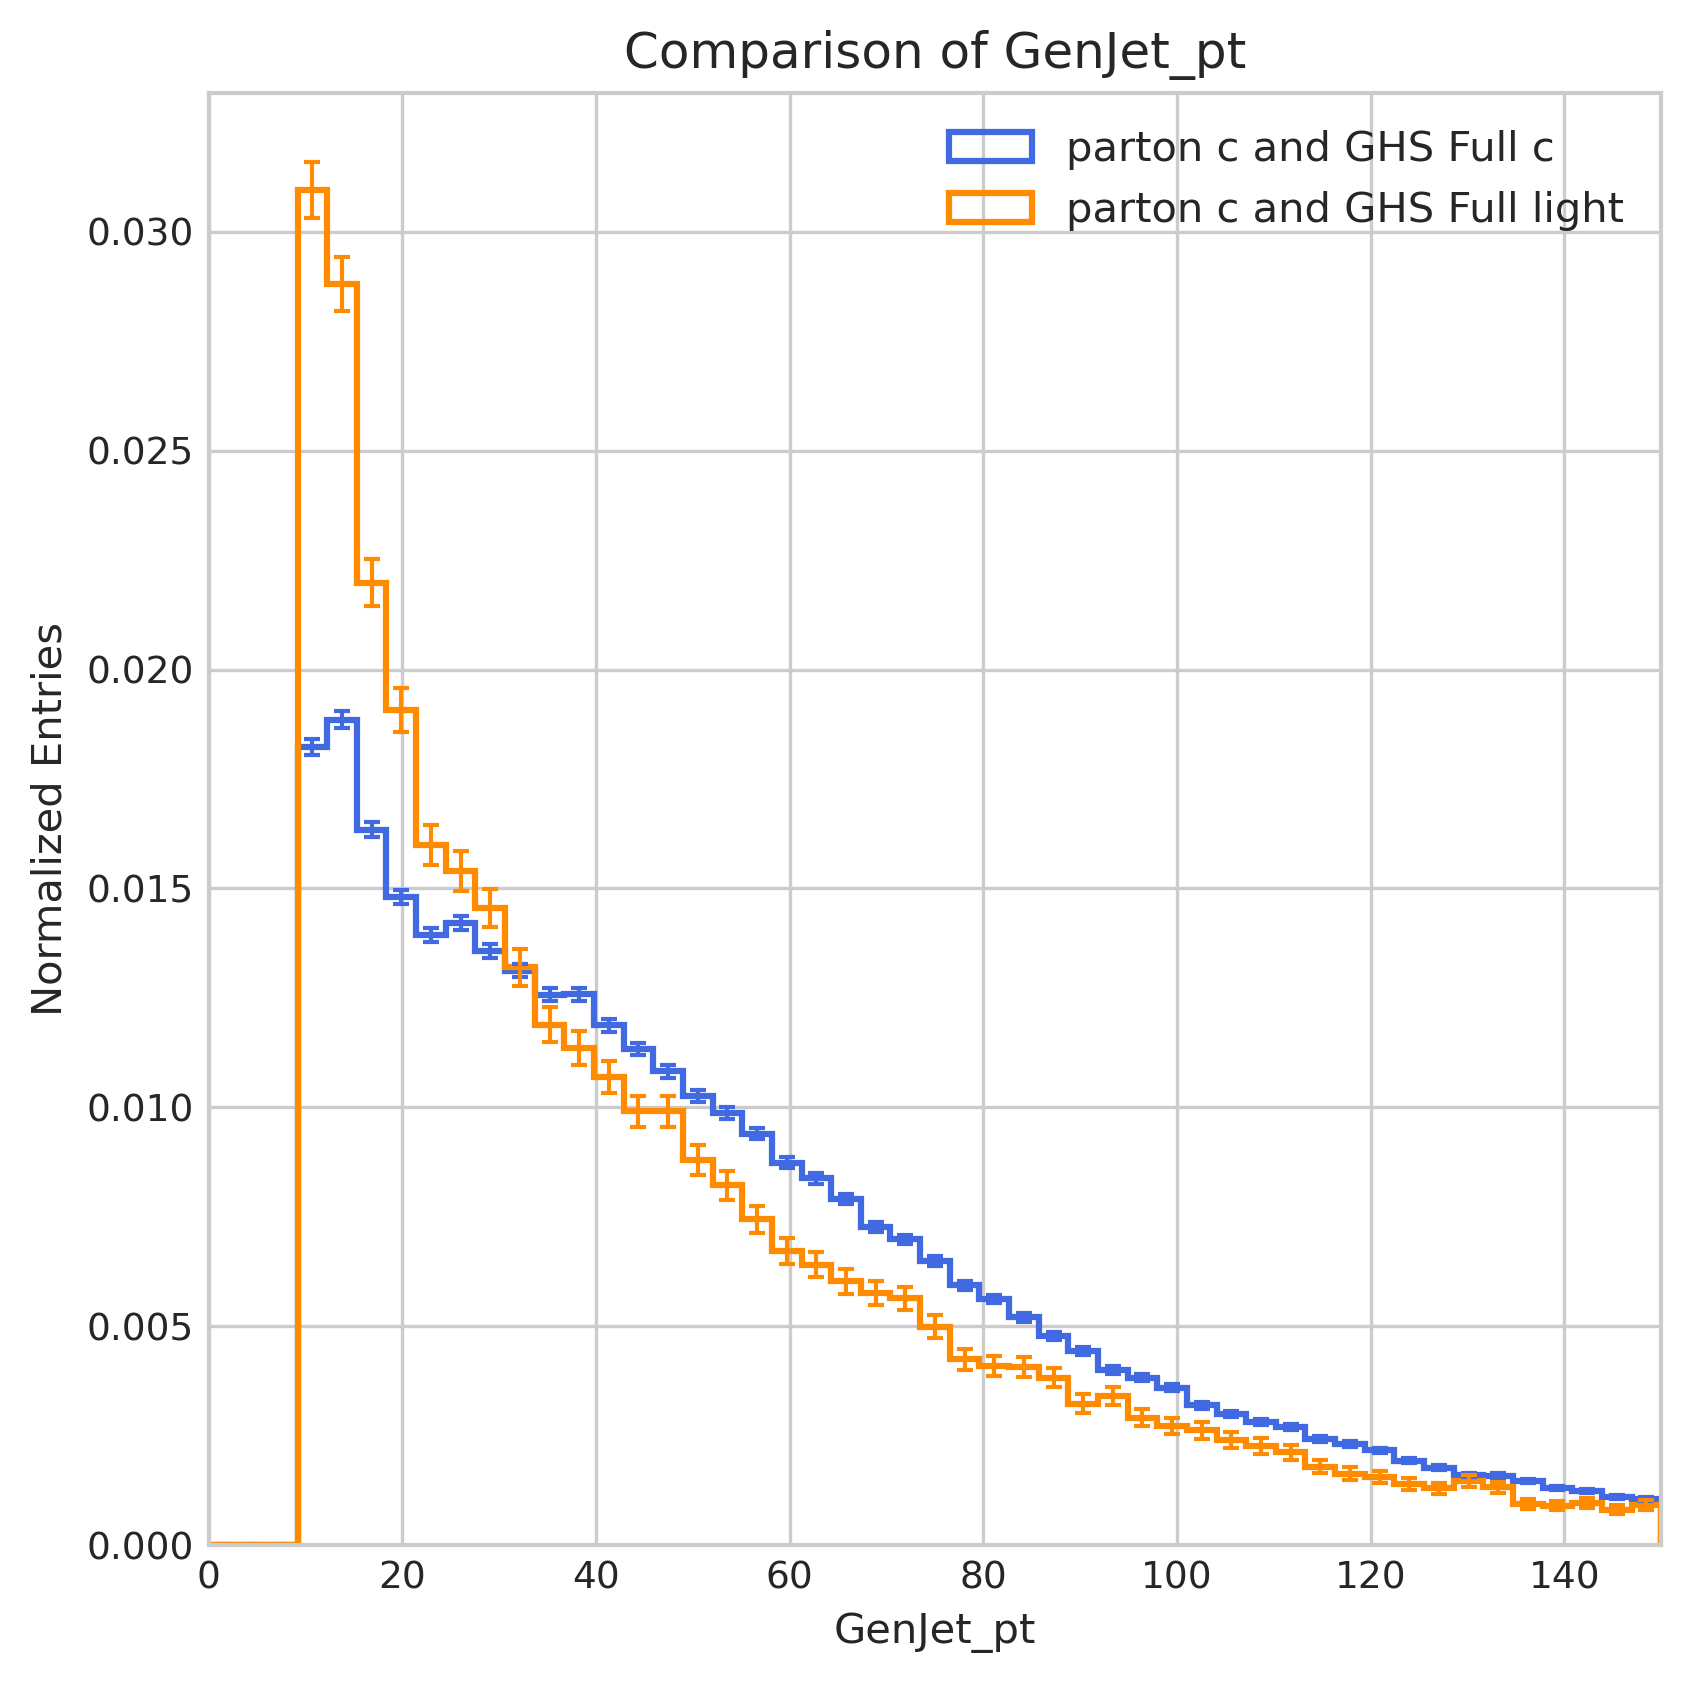
\includegraphics[width=\textwidth]{images/compare_GenJet_pt_GHSFull_light_vs_c_filter_partonFlavour_4.png}
        \caption{Generator-level c-jets}
        \label{fig:pt_c_parton_gen}
    \end{subfigure}
    \caption{Distributions of transverse momentum ($p_T$) for jets identified as c-jets by the $\parFlav$ definition. The comparison is between two categories: jets also identified as c-flavour by the GHS algorithm (blue) and those classified as light-flavour by GHS (orange). The distributions are normalized to unit area for shape comparison. (\subref{fig:pt_c_parton_full}) Full-chain simulation; (\subref{fig:pt_c_parton_gen}) Generator-level.}
    \label{fig:pt_c_parton_combined}
\end{figure*}

Figure \ref{fig:pt_b_hadron_combined} shows the jet $p_T$ distributions for b-jets defined by $\hadFlav$, while Figure \ref{fig:pt_c_hadron_combined} shows the same for c-jets, both at generator level and reconstruction level. Figures \ref{fig:pt_b_parton_combined} and \ref{fig:pt_c_parton_combined} show the corresponding distributions for b- and c-jets defined by $\parFlav$.

In all cases, jets identified as heavy-flavour by both definitions exhibit harder $p_T$ spectra compared to those identified as heavy-flavour by conventional definitions but light by GHS, consistent with the expectation that genuine heavy-flavour jets should have higher $p_T$.

\subsubsection{Number of Associated Heavy-Flavour Hadrons for Generator-level Jets}
\label{sec:vali-vars-nhad}


\begin{figure*}[!htbp]
    \centering
    \begin{subfigure}[t]{0.48\textwidth}
        \centering
        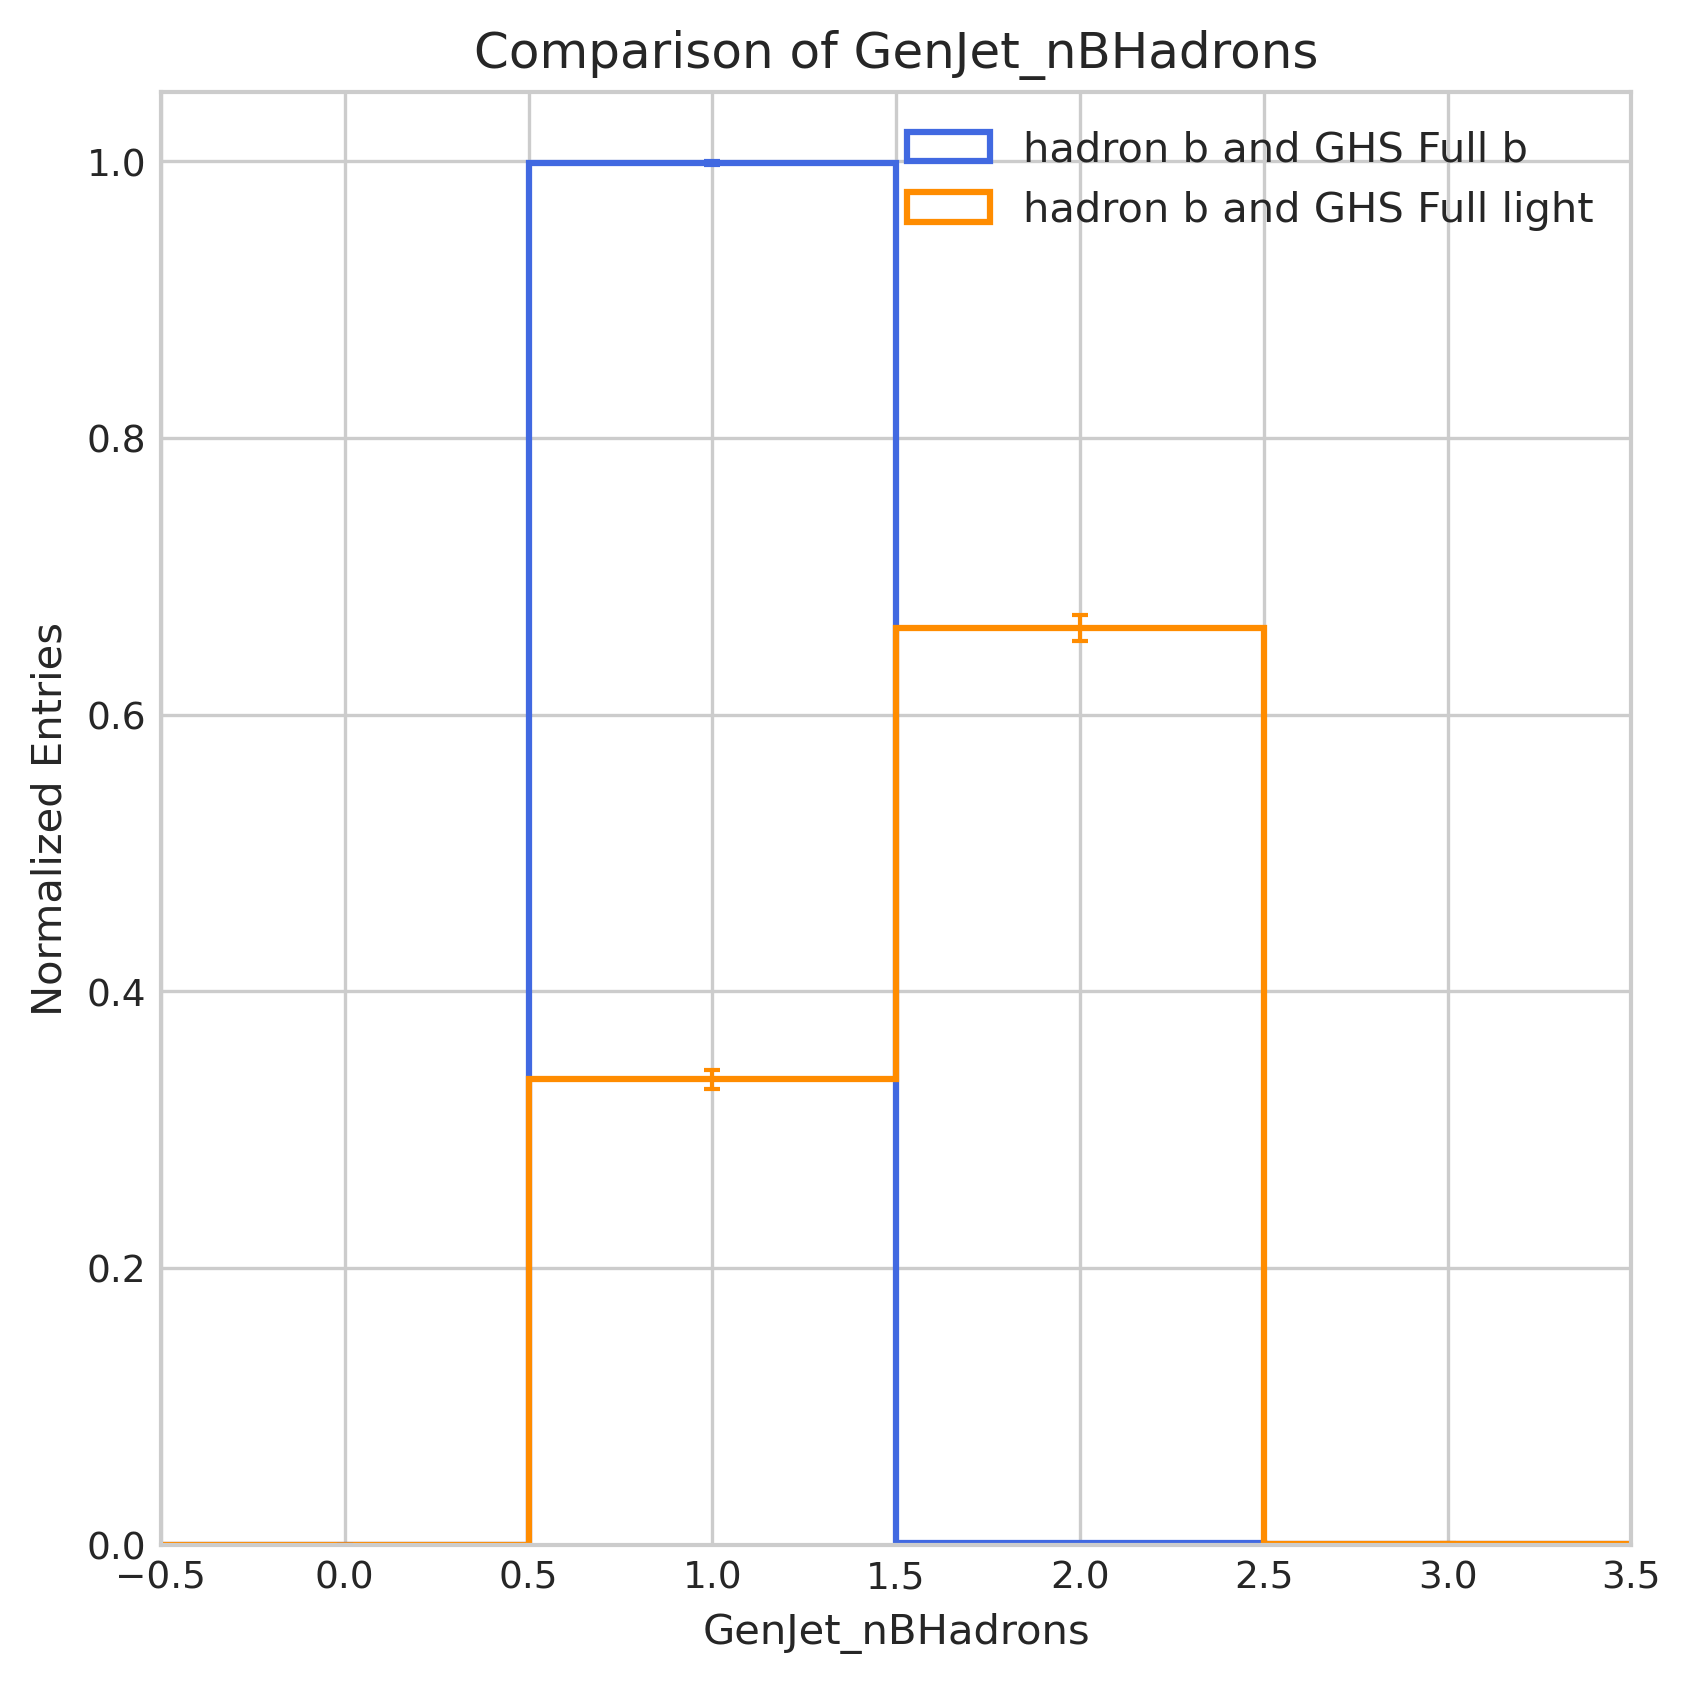
\includegraphics[width=\textwidth]{images/compare_GenJet_nBHadrons_GHSFull_light_vs_b_filter_hadronFlavour_5.png}
        \caption{b-jets defined by $\hadFlav$}
        \label{fig:GenJet_nBHad_full_b_hadron_b}
    \end{subfigure}
    \hfill
    \begin{subfigure}[t]{0.48\textwidth}
        \centering
        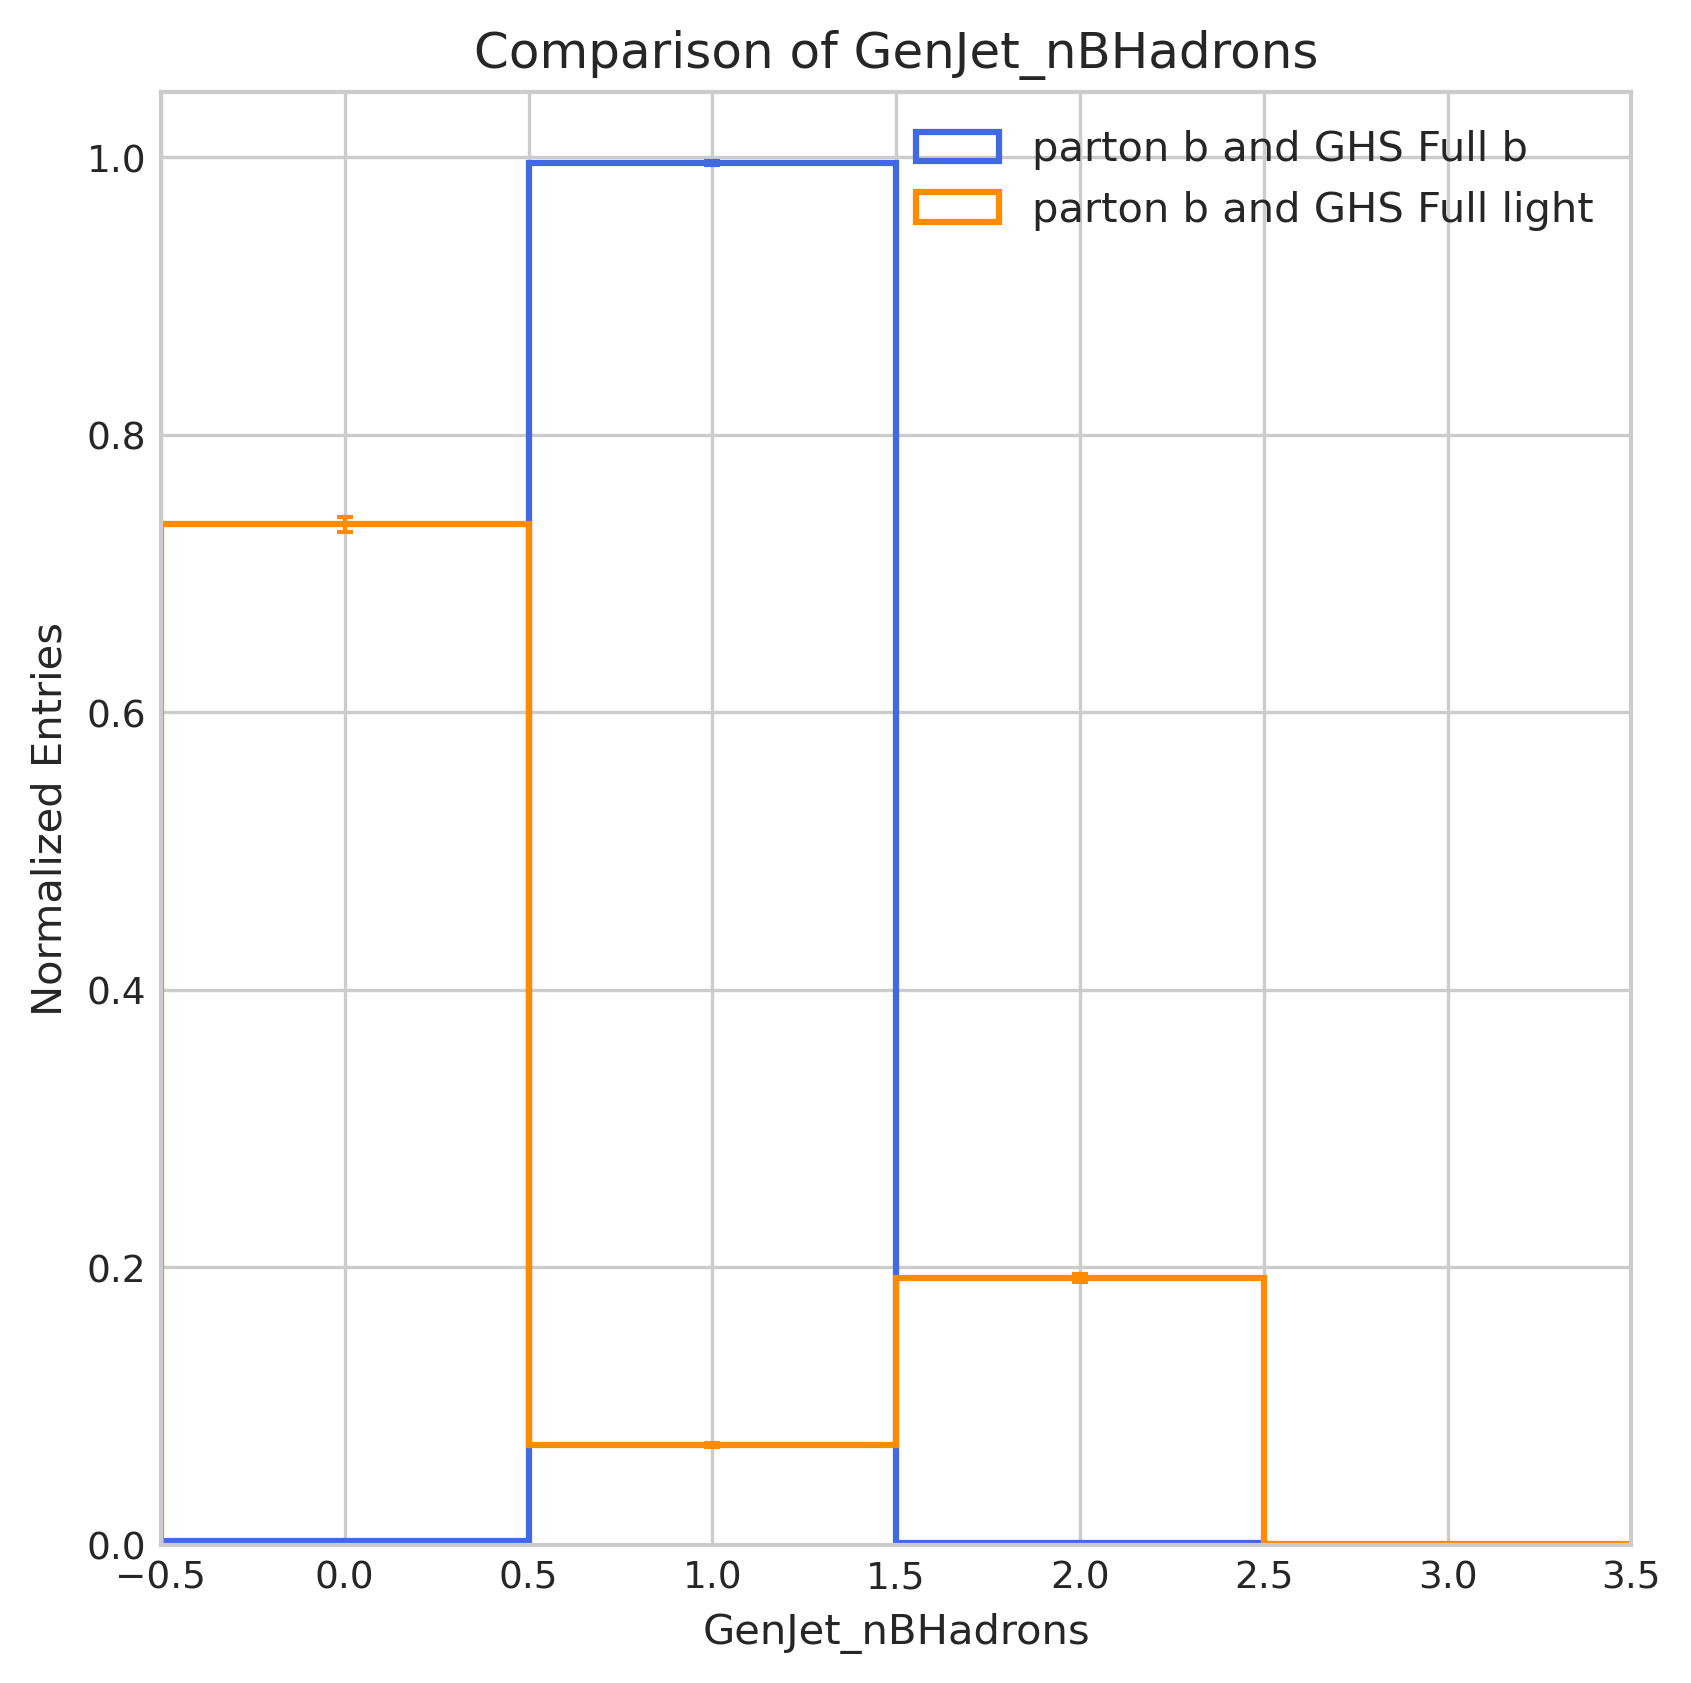
\includegraphics[width=\textwidth]{images/compare_GenJet_nBHadrons_GHSFull_light_vs_b_filter_partonFlavour_5.png}
        \caption{b-jets defined by $\parFlav$}
        \label{fig:GenJet_nBHad_full_b_parton_b}
    \end{subfigure}
    \caption{Distributions of the number of associated b-hadrons ($\texttt{nBHadrons}$) for generator-level jets. The comparison is between b-jets identified by both GHS and conventional definitions (blue) versus those identified as b-jets by $\hadFlav$ or $\parFlav$ but classified as light-flavour by GHS (orange). (\subref{fig:GenJet_nBHad_full_b_hadron_b}) b-jets defined by $\hadFlav$; (\subref{fig:GenJet_nBHad_full_b_parton_b}) b-jets defined by $\parFlav$.}
    \label{fig:GenJet_nBHad}
\end{figure*}

In b-jets defined by both GHS and conventional definitions, a significantly higher proportion of jets contain exactly one b-hadron is observed, as shown in Figure \ref{fig:GenJet_nBHad}. While in jets identified as b-jets by conventional definitions but light by GHS, a large fraction of jets contain two or more b-hadrons, or no b-hadrons at all for $\parFlav$-b jets.

\begin{figure*}[!htbp]
    \centering
    \begin{subfigure}[t]{0.48\textwidth}
        \centering
        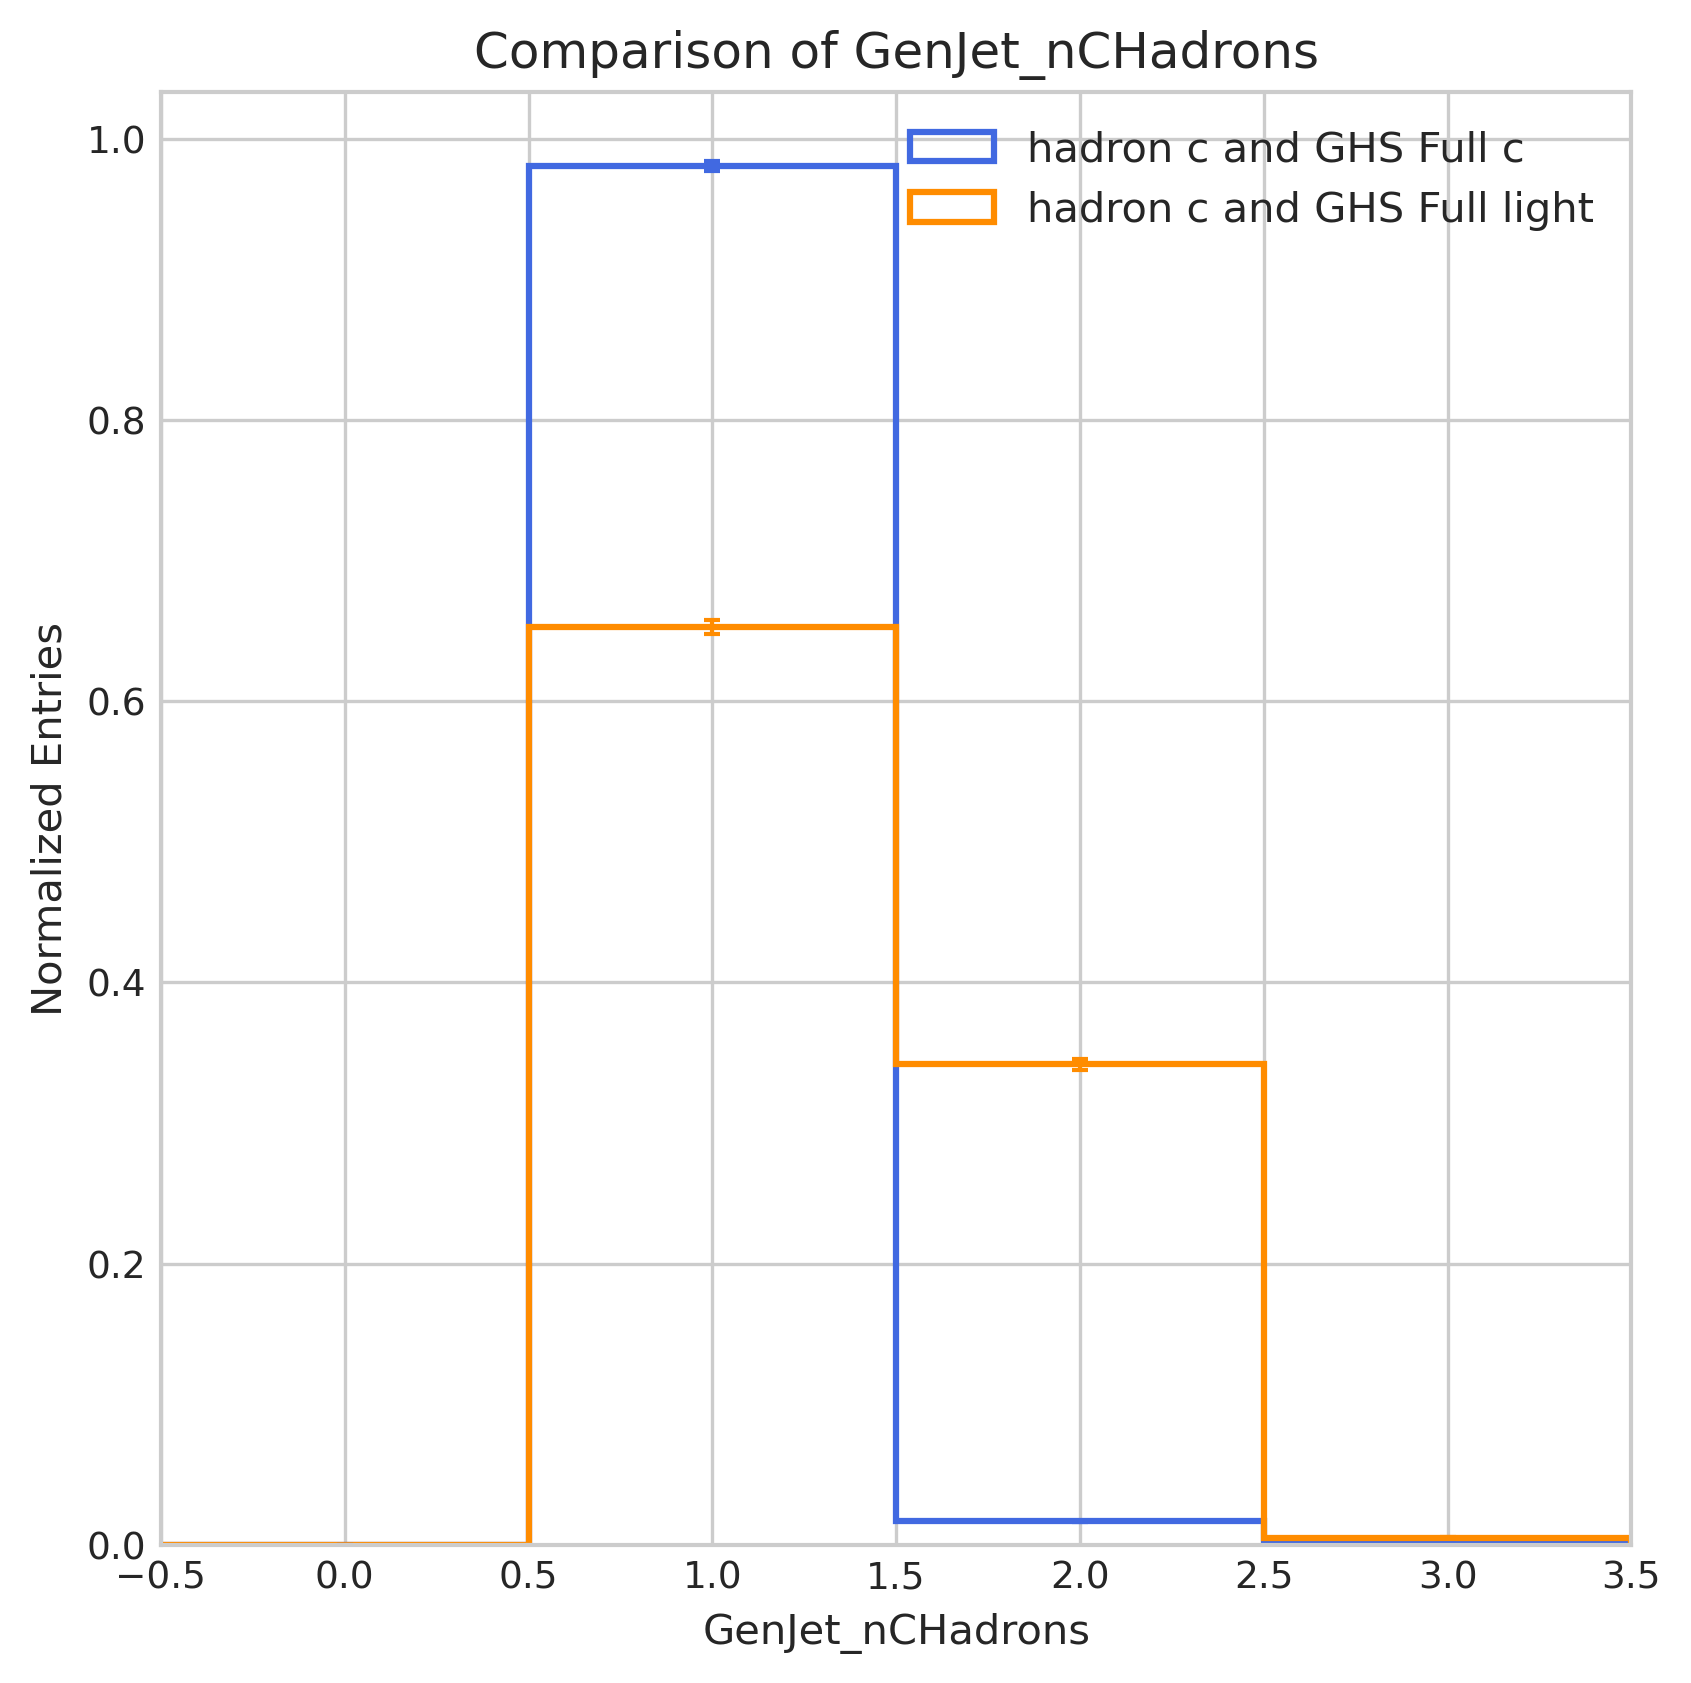
\includegraphics[width=\textwidth]{images/compare_GenJet_nCHadrons_GHSFull_light_vs_c_filter_hadronFlavour_4.png}
        \caption{c-jets defined by $\hadFlav$}
        \label{fig:GenJet_nCHad_full_c_hadron_c}
    \end{subfigure}
    \hfill
    \begin{subfigure}[t]{0.48\textwidth}
        \centering
        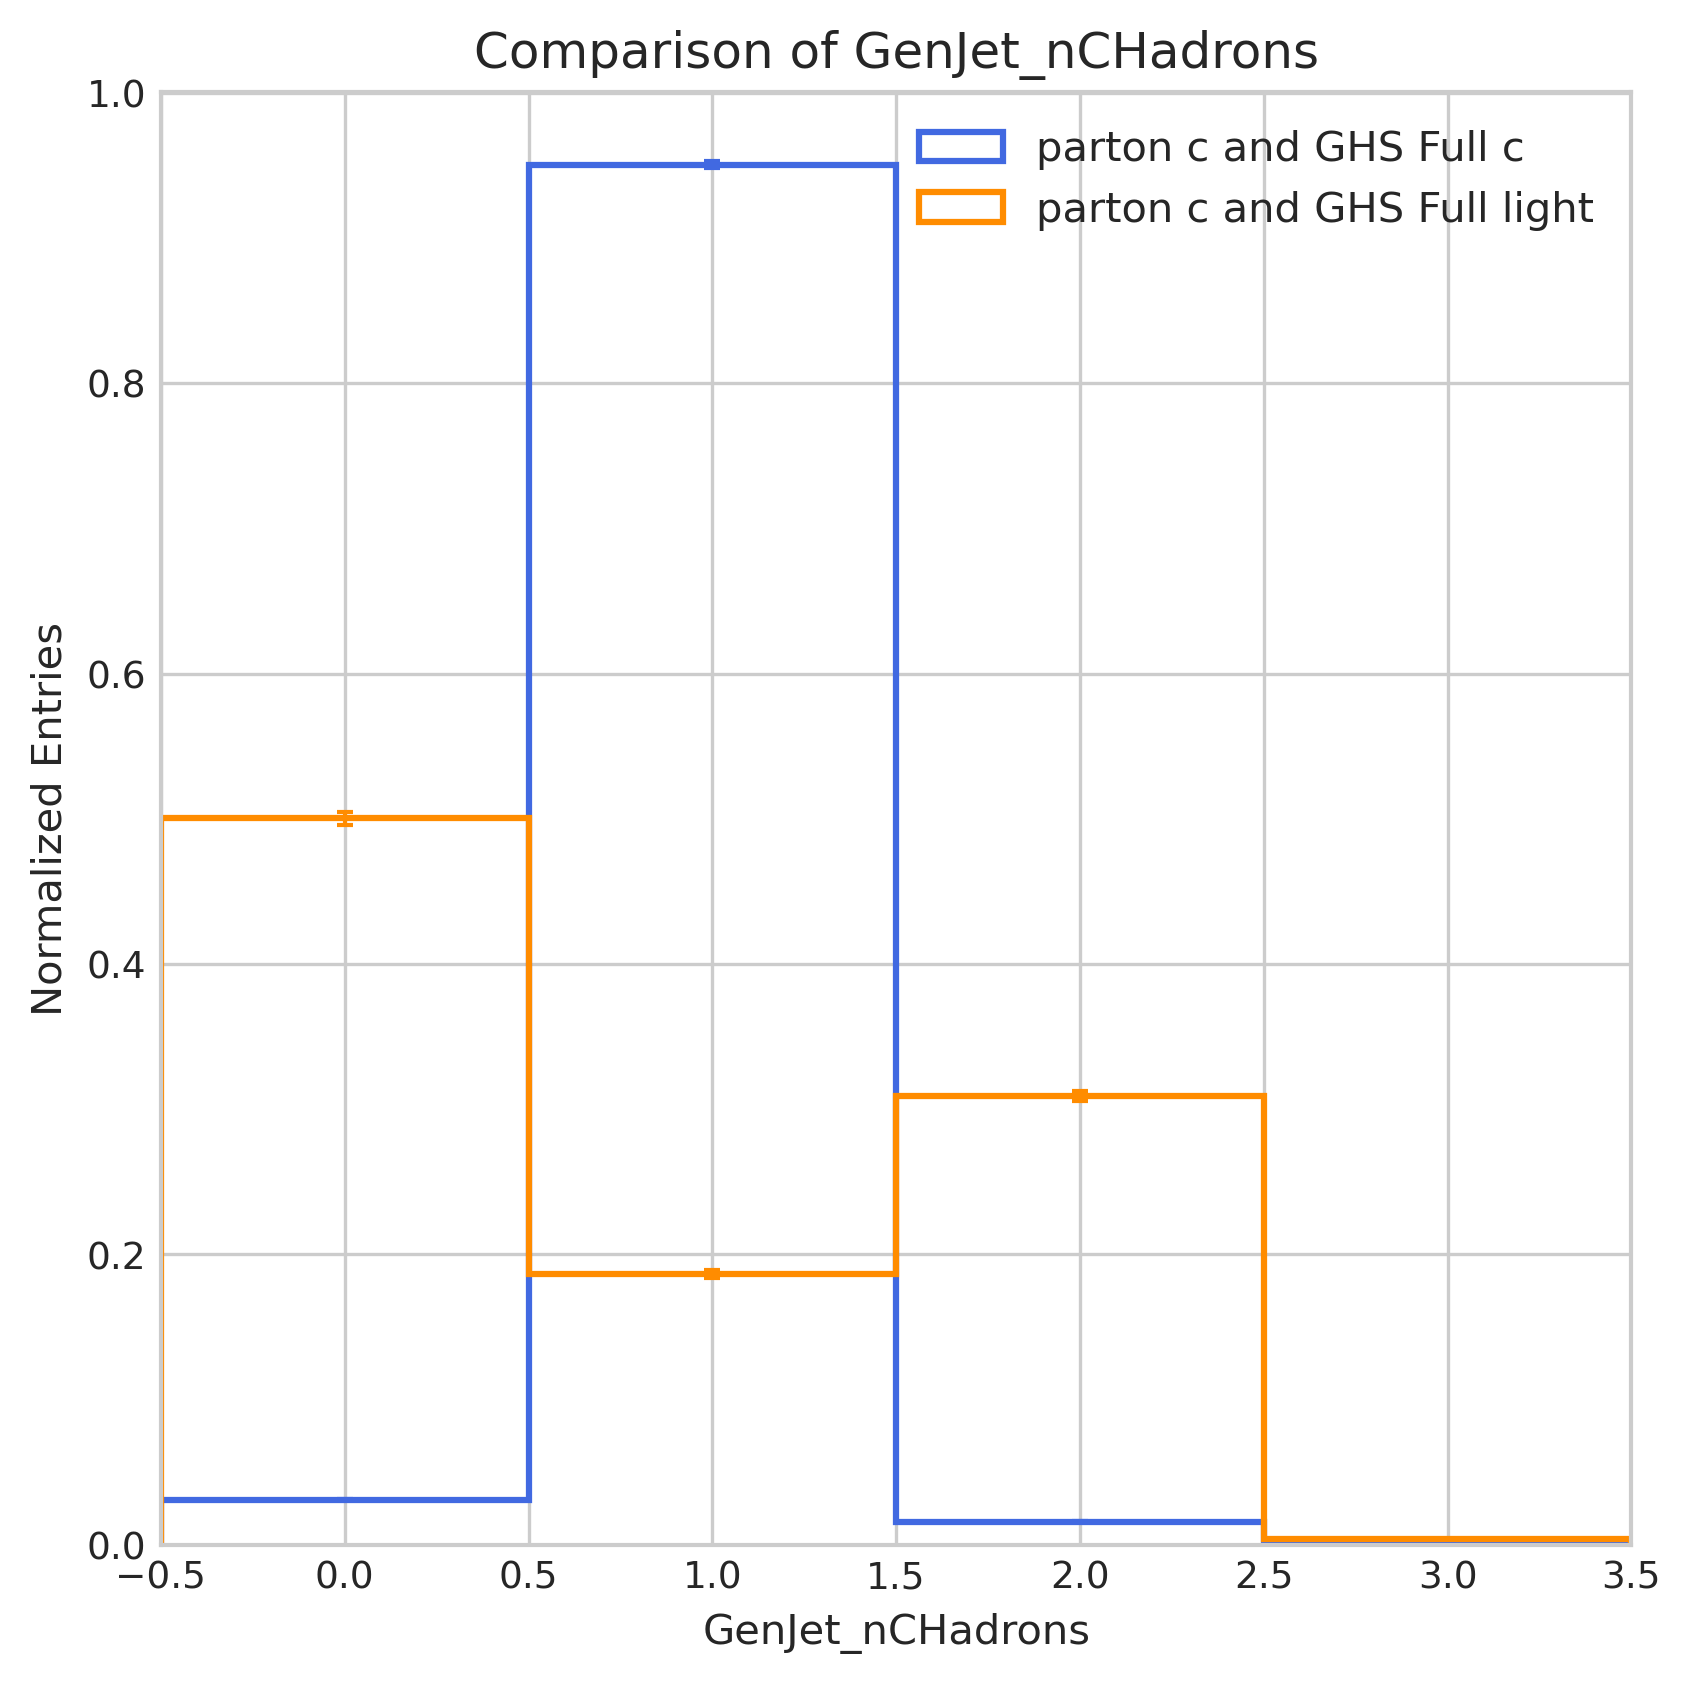
\includegraphics[width=\textwidth]{images/compare_GenJet_nCHadrons_GHSFull_light_vs_c_filter_partonFlavour_4.png}
        \caption{c-jets defined by $\parFlav$}
        \label{fig:GenJet_nCHad_full_c_parton_c}
    \end{subfigure}
    \caption{Distributions of the number of associated c-hadrons ($\texttt{nCHadrons}$) for generator-level jets. The comparison is between c-jets identified by both GHS and conventional definitions (blue) versus those identified as c-jets by $\hadFlav$ or $\parFlav$ but classified as light-flavour by GHS (orange). (\subref{fig:GenJet_nCHad_full_c_hadron_c}) c-jets defined by $\hadFlav$; (\subref{fig:GenJet_nCHad_full_c_parton_c}) c-jets defined by $\parFlav$.}
    \label{fig:GenJet_nCHad}
\end{figure*}

In c-jets, similar trends are observed in Figure \ref{fig:GenJet_nCHad}, with a lower proportion of jets containing exactly one c-hadron in jets identified as c-jets by both conventional definitions and GHS.

The results shown above are consistent with the expectation that genuine heavy-flavour jets should contain exactly one heavy-flavour hadron. Those jets identified as heavy-flavour by $\parFlav$ yet containing no heavy-flavour hadrons are likely coming from soft heavy-flavour quark contamination, with the corresponding hadron further "recoiled" away from the jet axis during hadronization. Those jets containing two or more heavy-flavour hadrons are likely originating from gluon splitting into a heavy-quark pair ($g \to b\bar{b}$ or $g \to c\bar{c}$).

\subsubsection{Number of Secondary Vertices in Reconstructed Jets}
\label{sec:vali-vars-nsv}

\begin{figure*}[!htbp]
    \centering
    \begin{subfigure}[t]{0.48\textwidth}
        \centering
        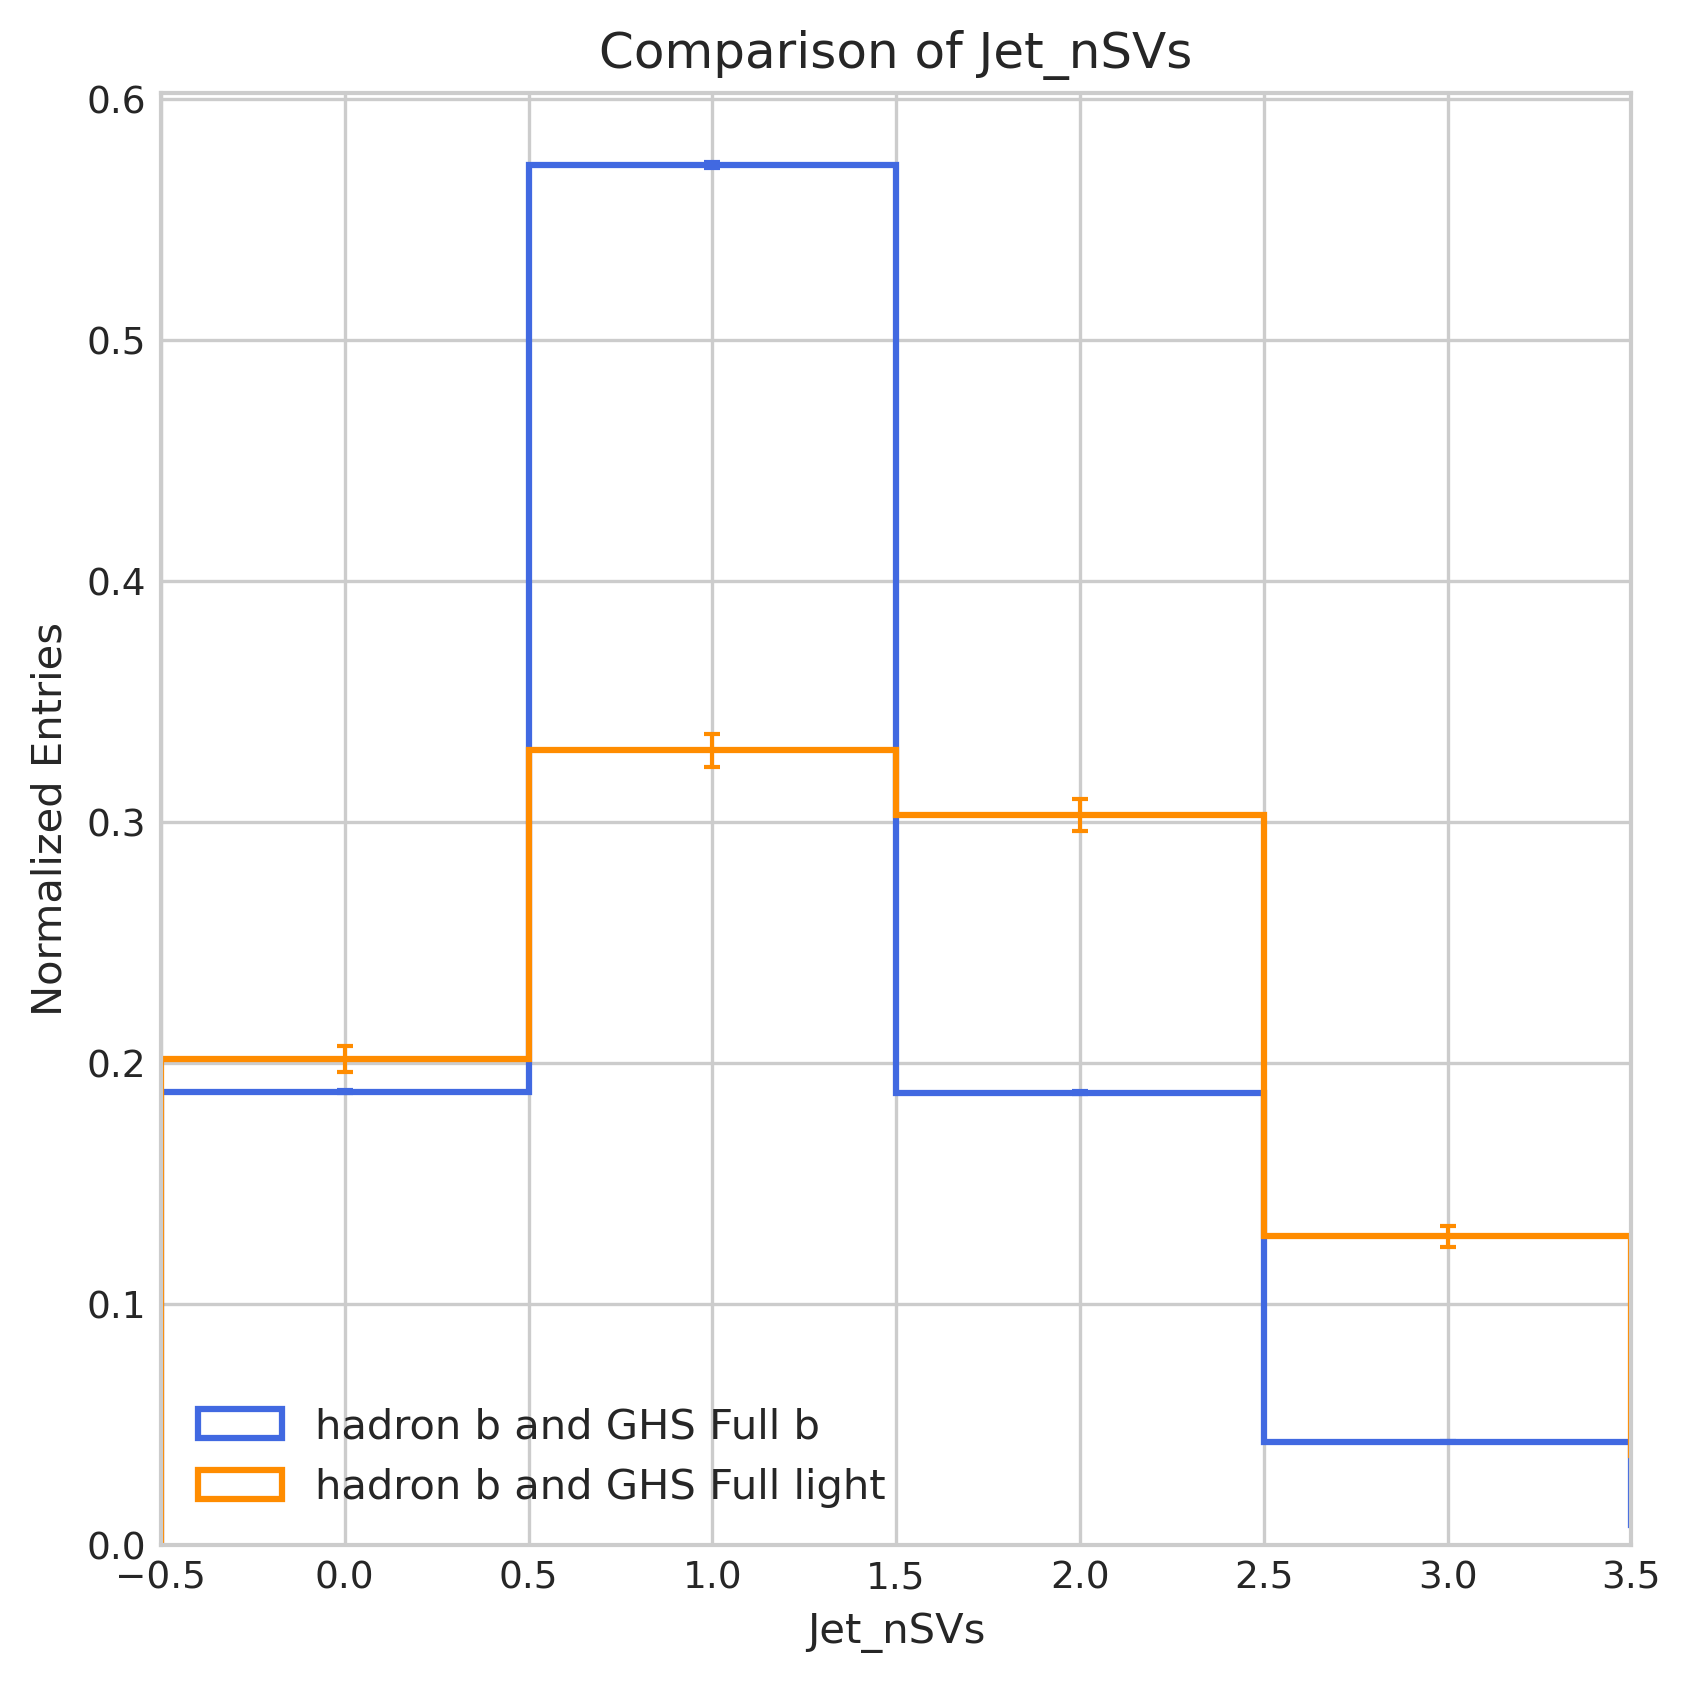
\includegraphics[width=\textwidth]{images/compare_nSVs_GHSFull_light_vs_b_filter_hadronFlavour_5.png}
        \caption{b-jets defined by $\hadFlav$}
        \label{fig:jet_nSVs_full_b_hadron_b}
    \end{subfigure}
    \hfill
    \begin{subfigure}[t]{0.48\textwidth}
        \centering
        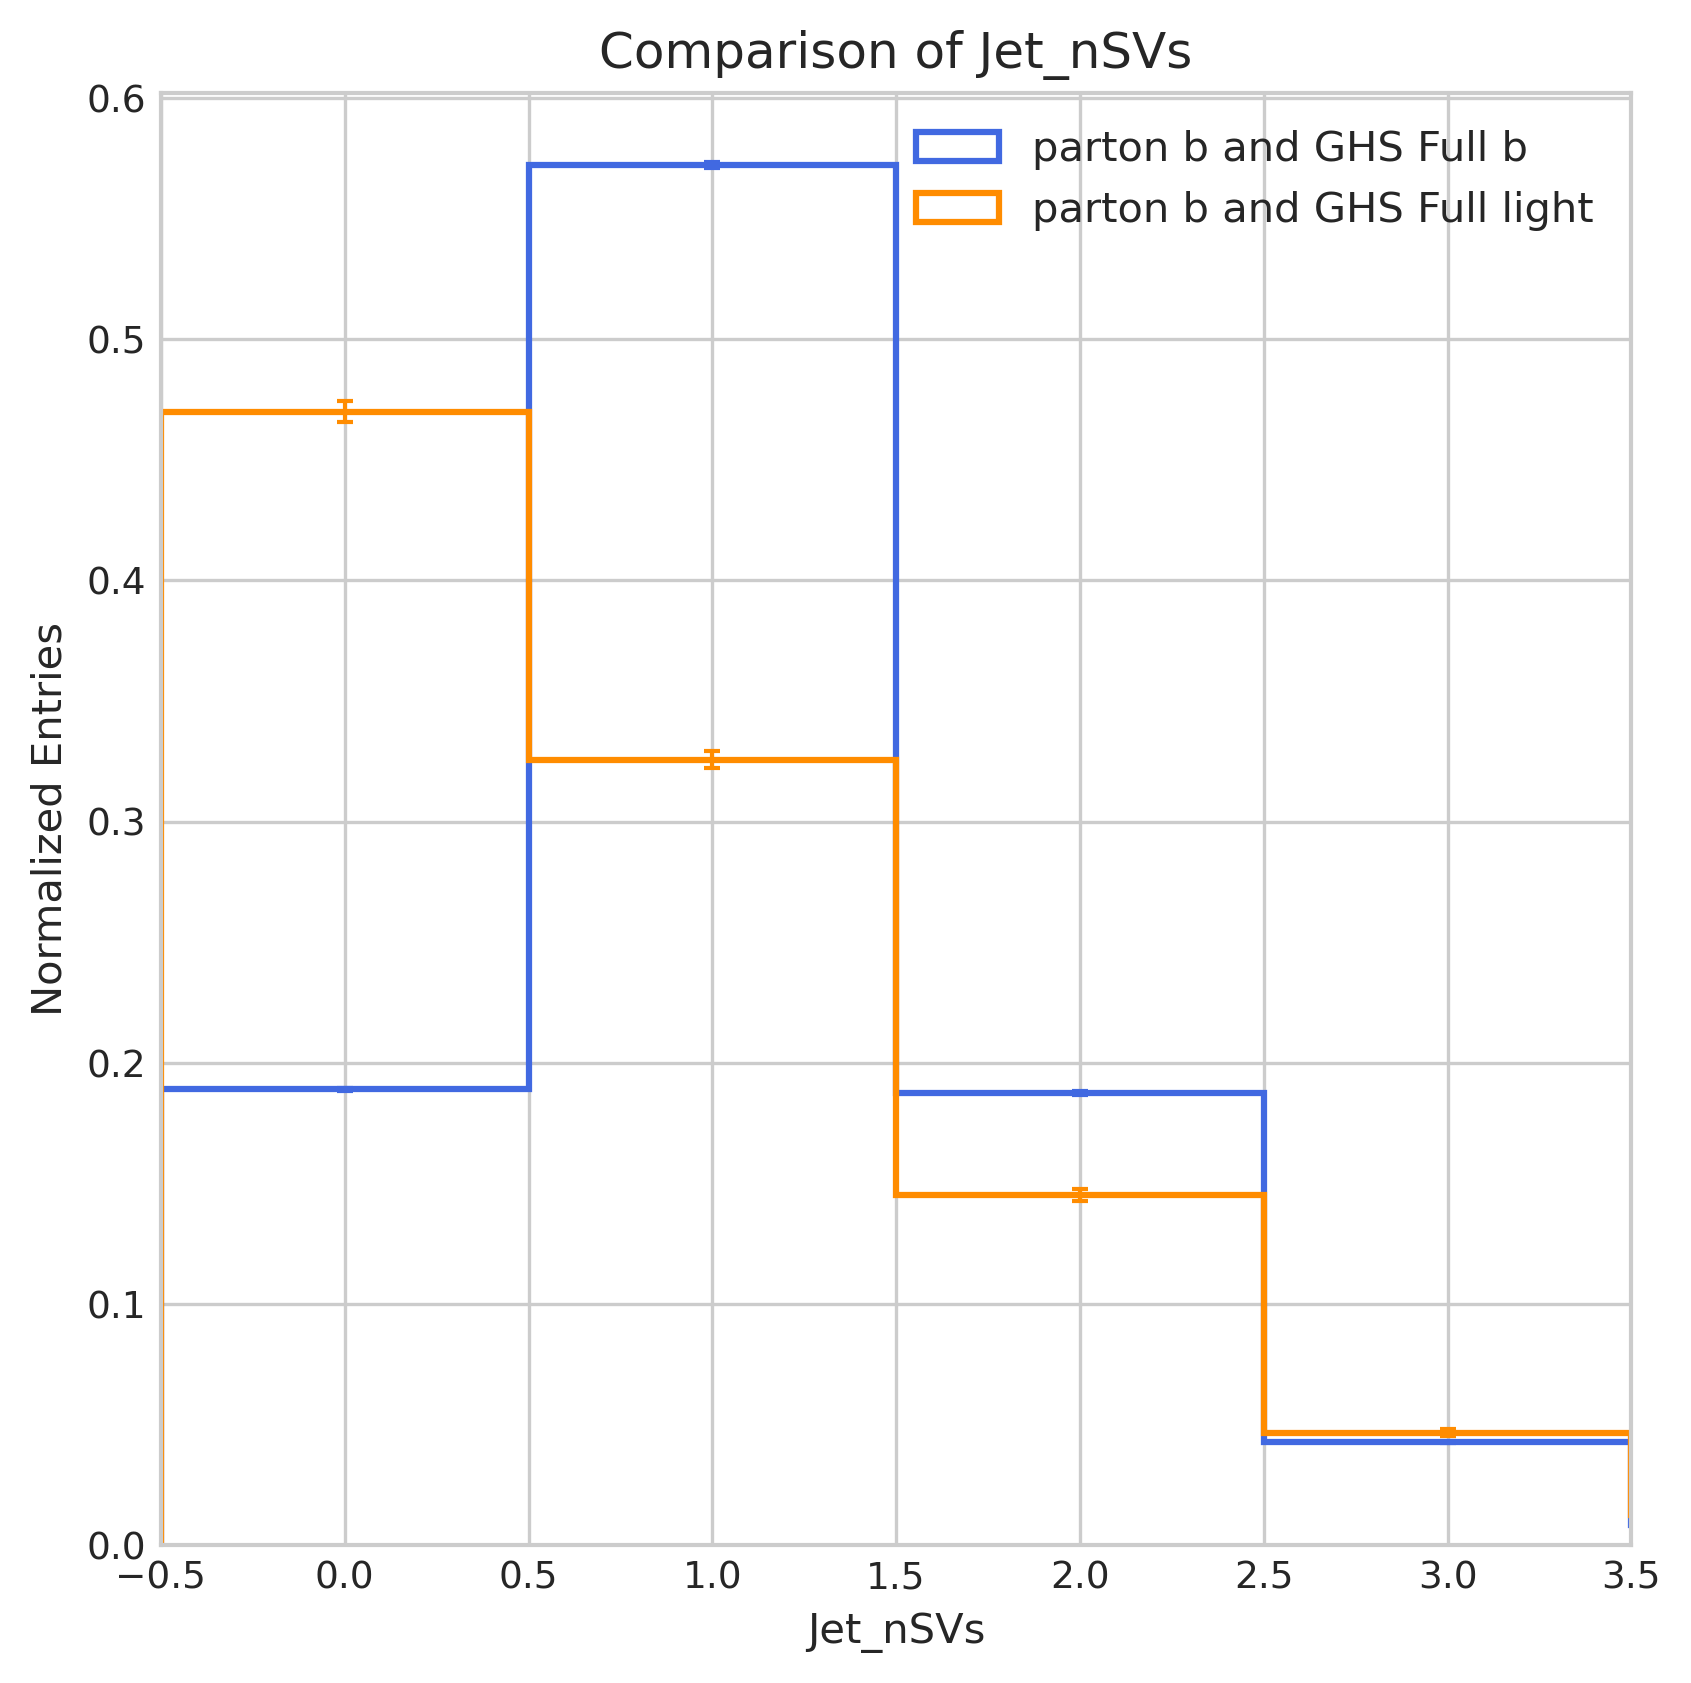
\includegraphics[width=\textwidth]{images/compare_nSVs_GHSFull_light_vs_b_filter_partonFlavour_5.png}
        \caption{b-jets defined by $\parFlav$}
        \label{fig:jet_nSVs_full_b_parton_b}
    \end{subfigure}
    \caption{Distributions of the number of secondary vertices ($\texttt{nSVs}$) in reconstructed jets. The comparison is between b-jets identified by both GHS and conventional definitions (blue) versus those identified as b-jets by $\hadFlav$ or $\parFlav$ but classified as light-flavour by GHS (orange). (\subref{fig:jet_nSVs_full_b_hadron_b}) b-jets defined by $\hadFlav$; (\subref{fig:jet_nSVs_full_b_parton_b}) b-jets defined by $\parFlav$.}
    \label{fig:jet_nSVs_full_b}
\end{figure*}

In Figure \ref{fig:jet_nSVs_full_b}, b-jets defined by both GHS and conventional definitions are observed to have a significantly higher proportion of jets containing exactly one secondary vertex. For jets identified as b-jets by $\hadFlav$ but light by GHS, a larger fraction of jets contain two or more secondary vertices, while for jets identified as b-jets by $\parFlav$ but light by GHS, a significant fraction of jets contain no secondary vertices at all. 

\begin{figure*}[!htbp]
    \centering
    \begin{subfigure}[t]{0.48\textwidth}
        \centering
        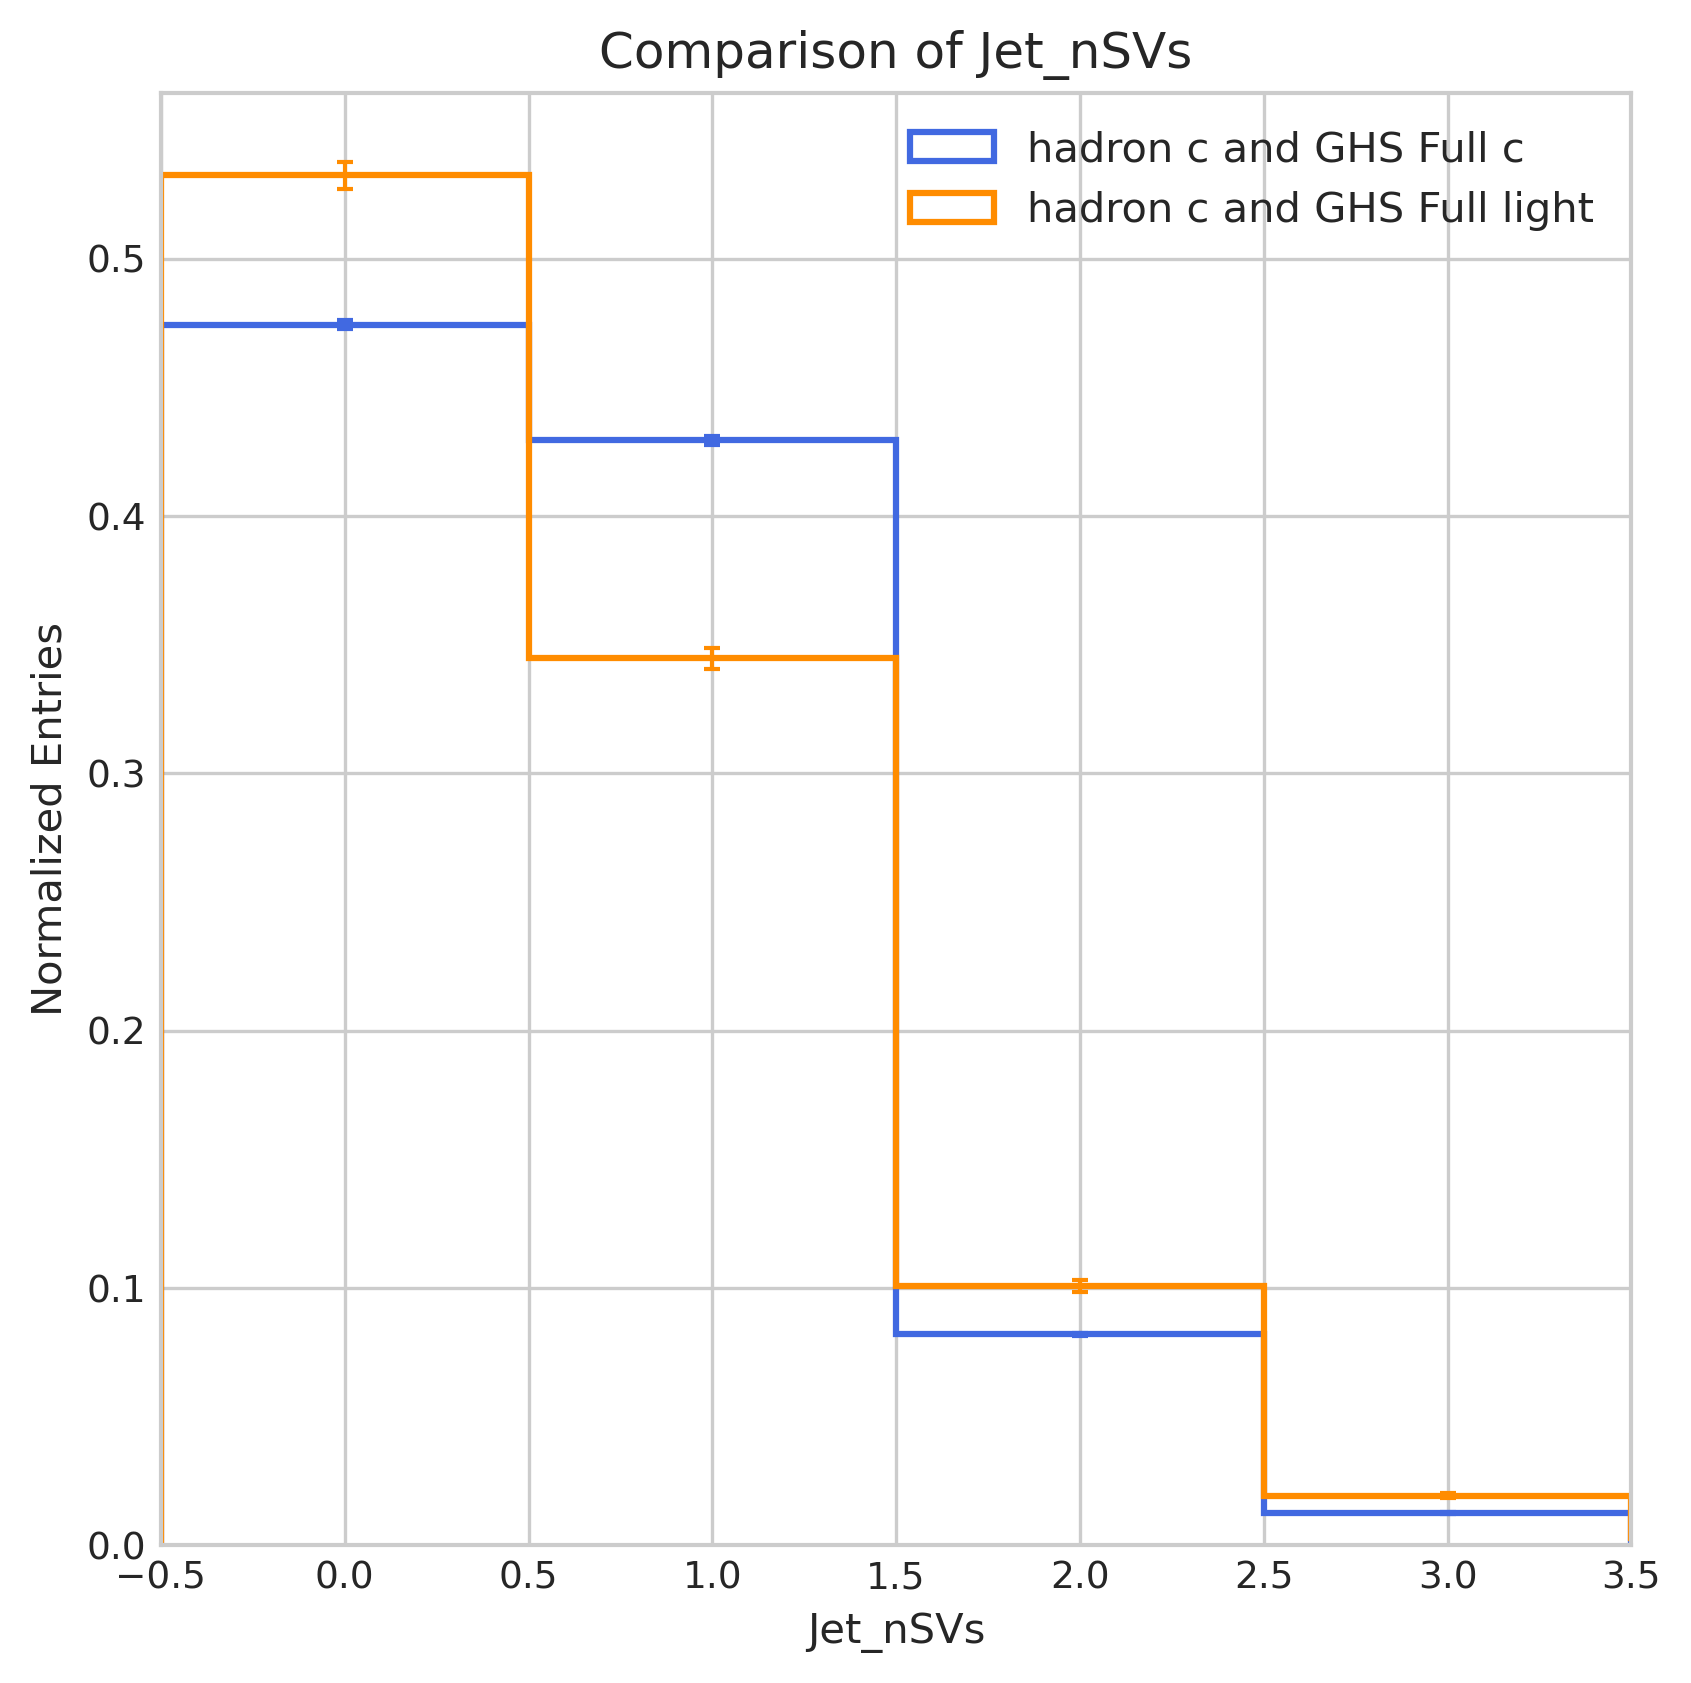
\includegraphics[width=\textwidth]{images/compare_nSVs_GHSFull_light_vs_c_filter_hadronFlavour_4.png}
        \caption{c-jets defined by $\hadFlav$}
        \label{fig:jet_nSVs_full_c_hadron_c}
    \end{subfigure}
    \hfill
    \begin{subfigure}[t]{0.48\textwidth}
        \centering
        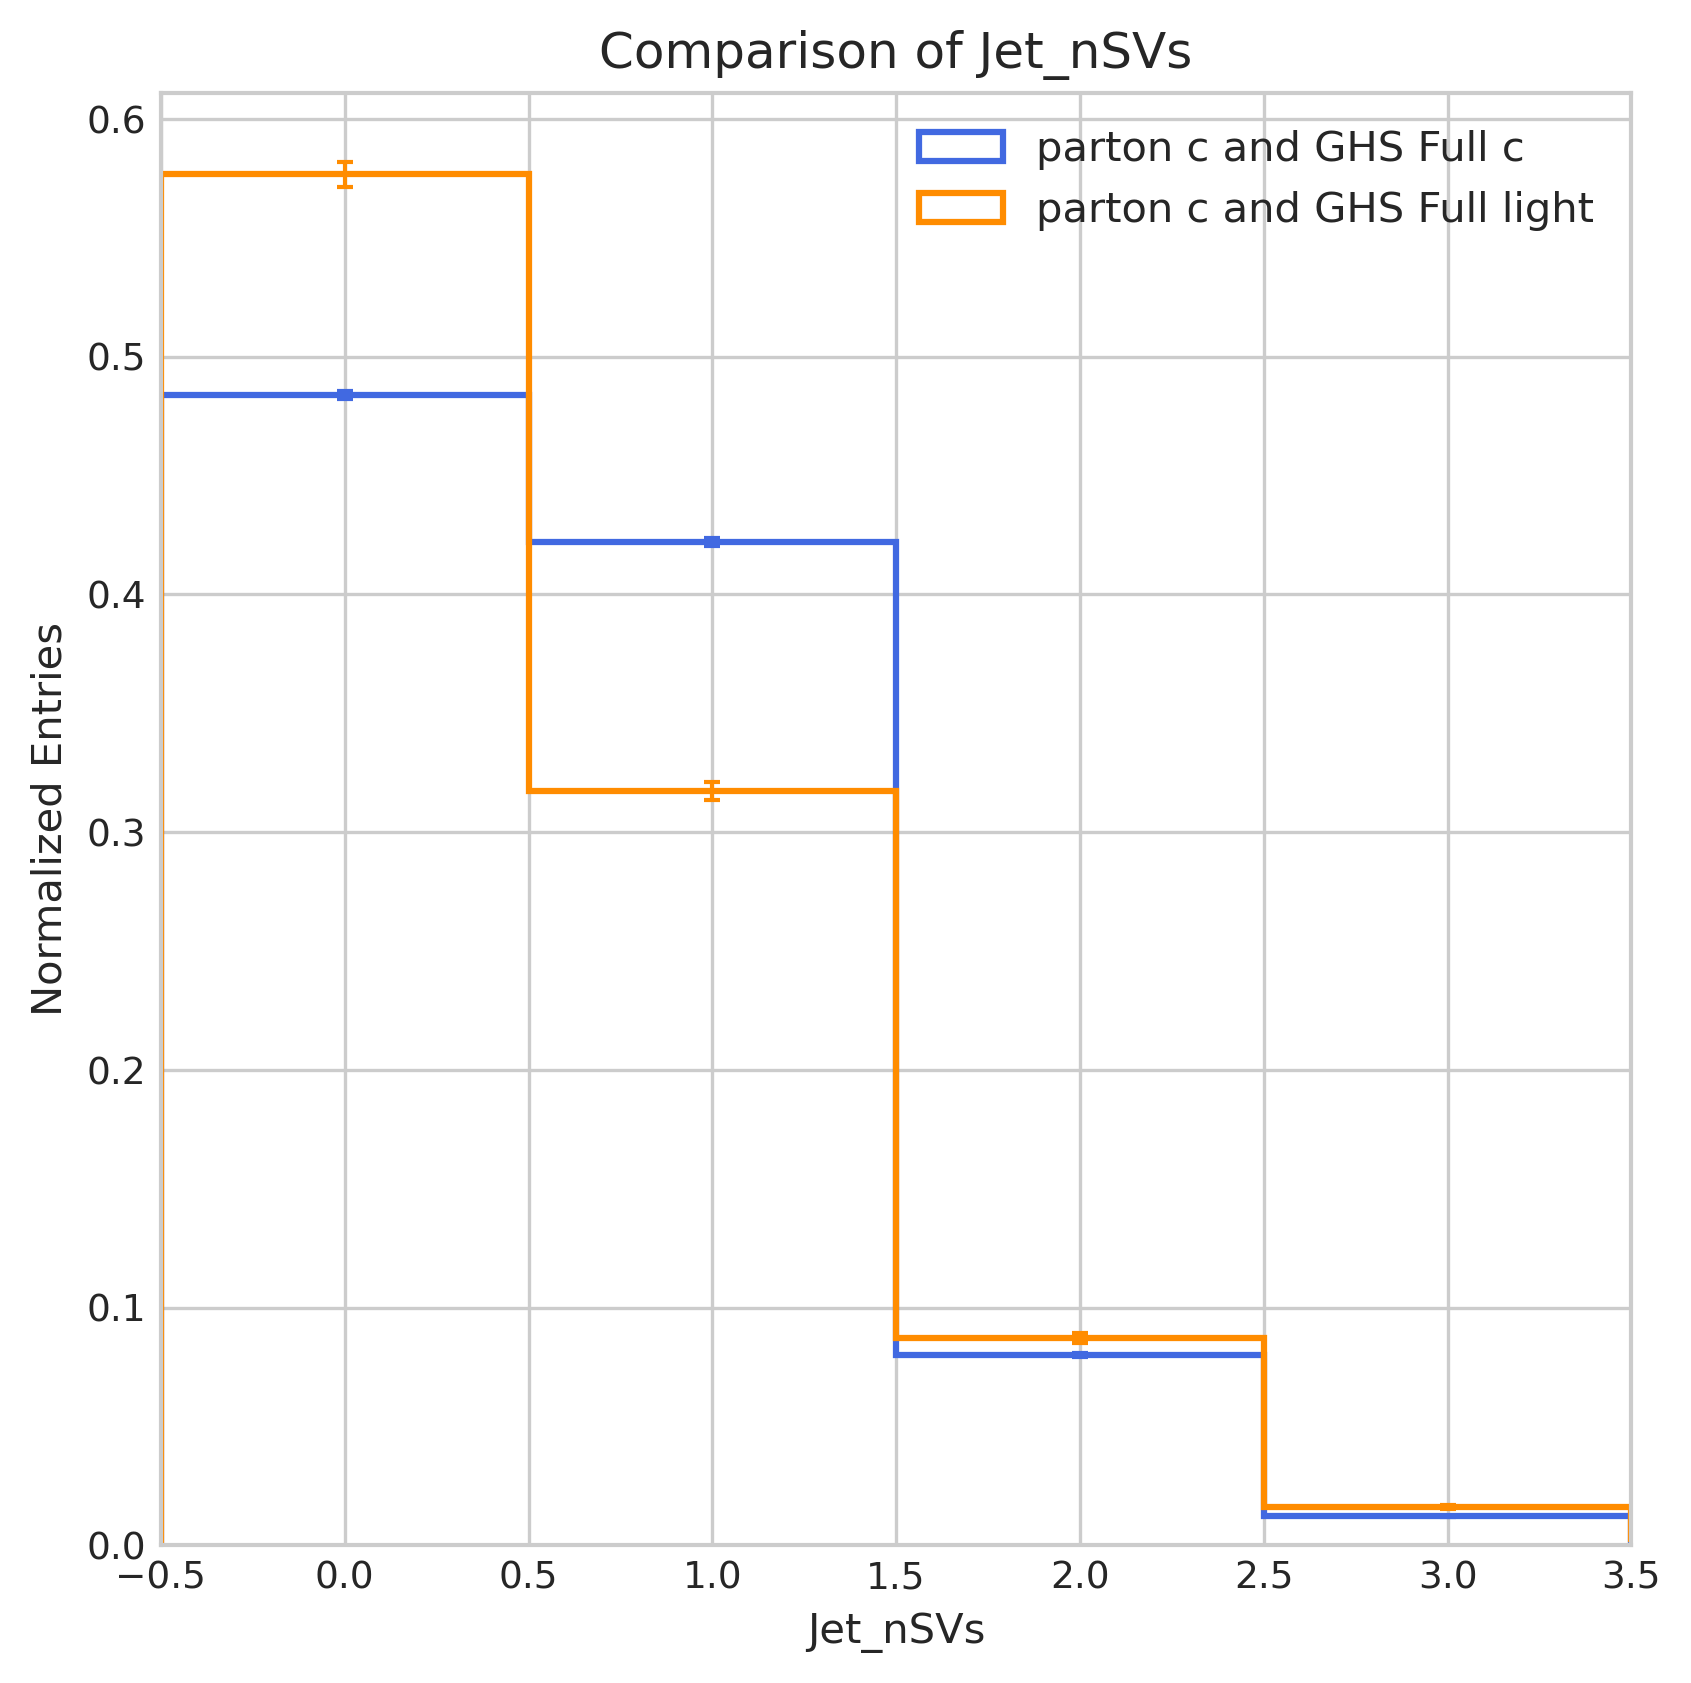
\includegraphics[width=\textwidth]{images/compare_nSVs_GHSFull_light_vs_c_filter_partonFlavour_4.png}
        \caption{c-jets defined by $\parFlav$}
        \label{fig:jet_nSVs_full_c_parton_c}
    \end{subfigure}
    \caption{Distributions of the number of secondary vertices ($\texttt{nSVs}$) in reconstructed jets. The comparison is between c-jets identified by both GHS and conventional definitions (blue) versus those identified as c-jets by $\hadFlav$ or $\parFlav$ but classified as light-flavour by GHS (orange). (\subref{fig:jet_nSVs_full_c_hadron_c}) c-jets defined by $\hadFlav$; (\subref{fig:jet_nSVs_full_c_parton_c}) c-jets defined by $\parFlav$.}
    \label{fig:jet_nSVs_full_c}
\end{figure*}

In c-jets, similar trends are observed in Figure \ref{fig:jet_nSVs_full_c}, yet the difference is less pronounced, with the majority of jets in both categories containing no secondary vertices. This is consistent with the shorter lifetimes of c-hadrons compared to b-hadrons, leading to fewer detectable secondary vertices.

In summary, the presence of secondary vertices within a jet is a strong indicator of heavy-flavour hadrons and thus the partonic origin of the jet. The results shown above are consistent with the expectation that genuine heavy-flavour jets should contain at least one secondary vertex, and also the comparison of number of associated heavy-flavour hadrons in generator-level jets as discussed in Section \ref{sec:vali-vars-nhad}.

\subsubsection{Flavour Tagging Scores in Reconstructed Jets}
\label{sec:vali-vars-ml}

The CMS implementation of \textsc{ParticleNet} \cite{quParticleNetJetTagging2020} and \textsc{ParticleTransformer} \cite{quParticleTransformerJet2024} produces the scores $\texttt{btagPNet}$ and $\texttt{btagParT}$, respectively, both ranging from 0 to 1, with higher values indicating a higher likelihood of the jet being a b-jet.

\begin{figure*}[!htbp]
    \centering
    \begin{subfigure}[t]{0.48\textwidth}
        \centering
        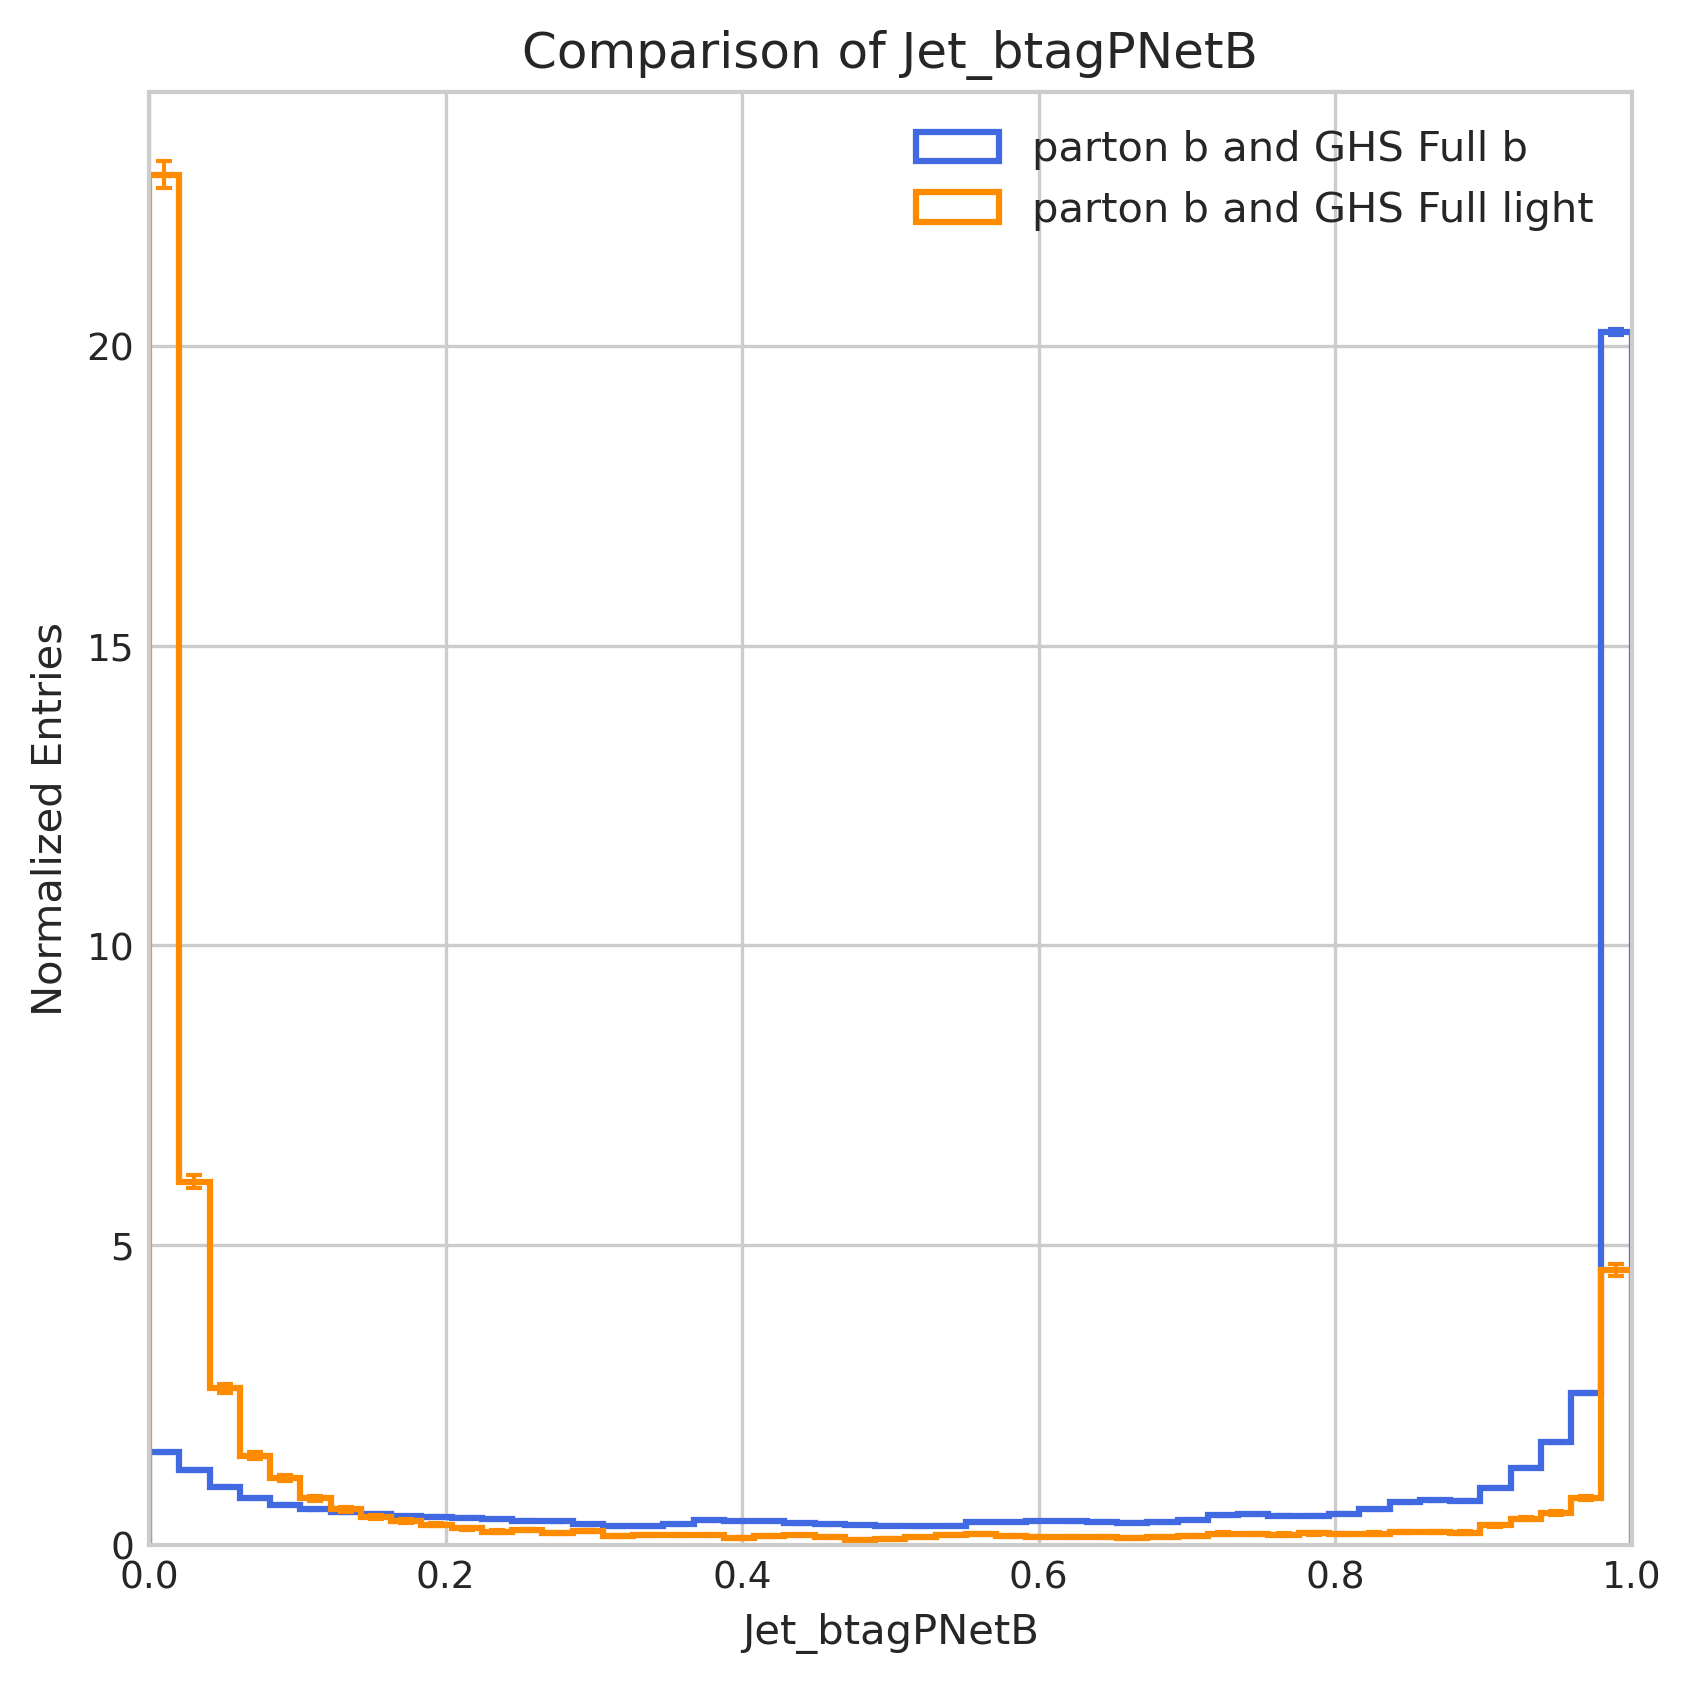
\includegraphics[width=\textwidth]{images/compare_btagPNetB_GHSFull_light_vs_b_filter_partonFlavour_5.png}
        \caption{b-tagging scores from \textsc{ParticleNet}}
        \label{fig:jet_btagPNet_full_b_parton_b}
    \end{subfigure}
    \hfill
    \begin{subfigure}[t]{0.48\textwidth}
        \centering
        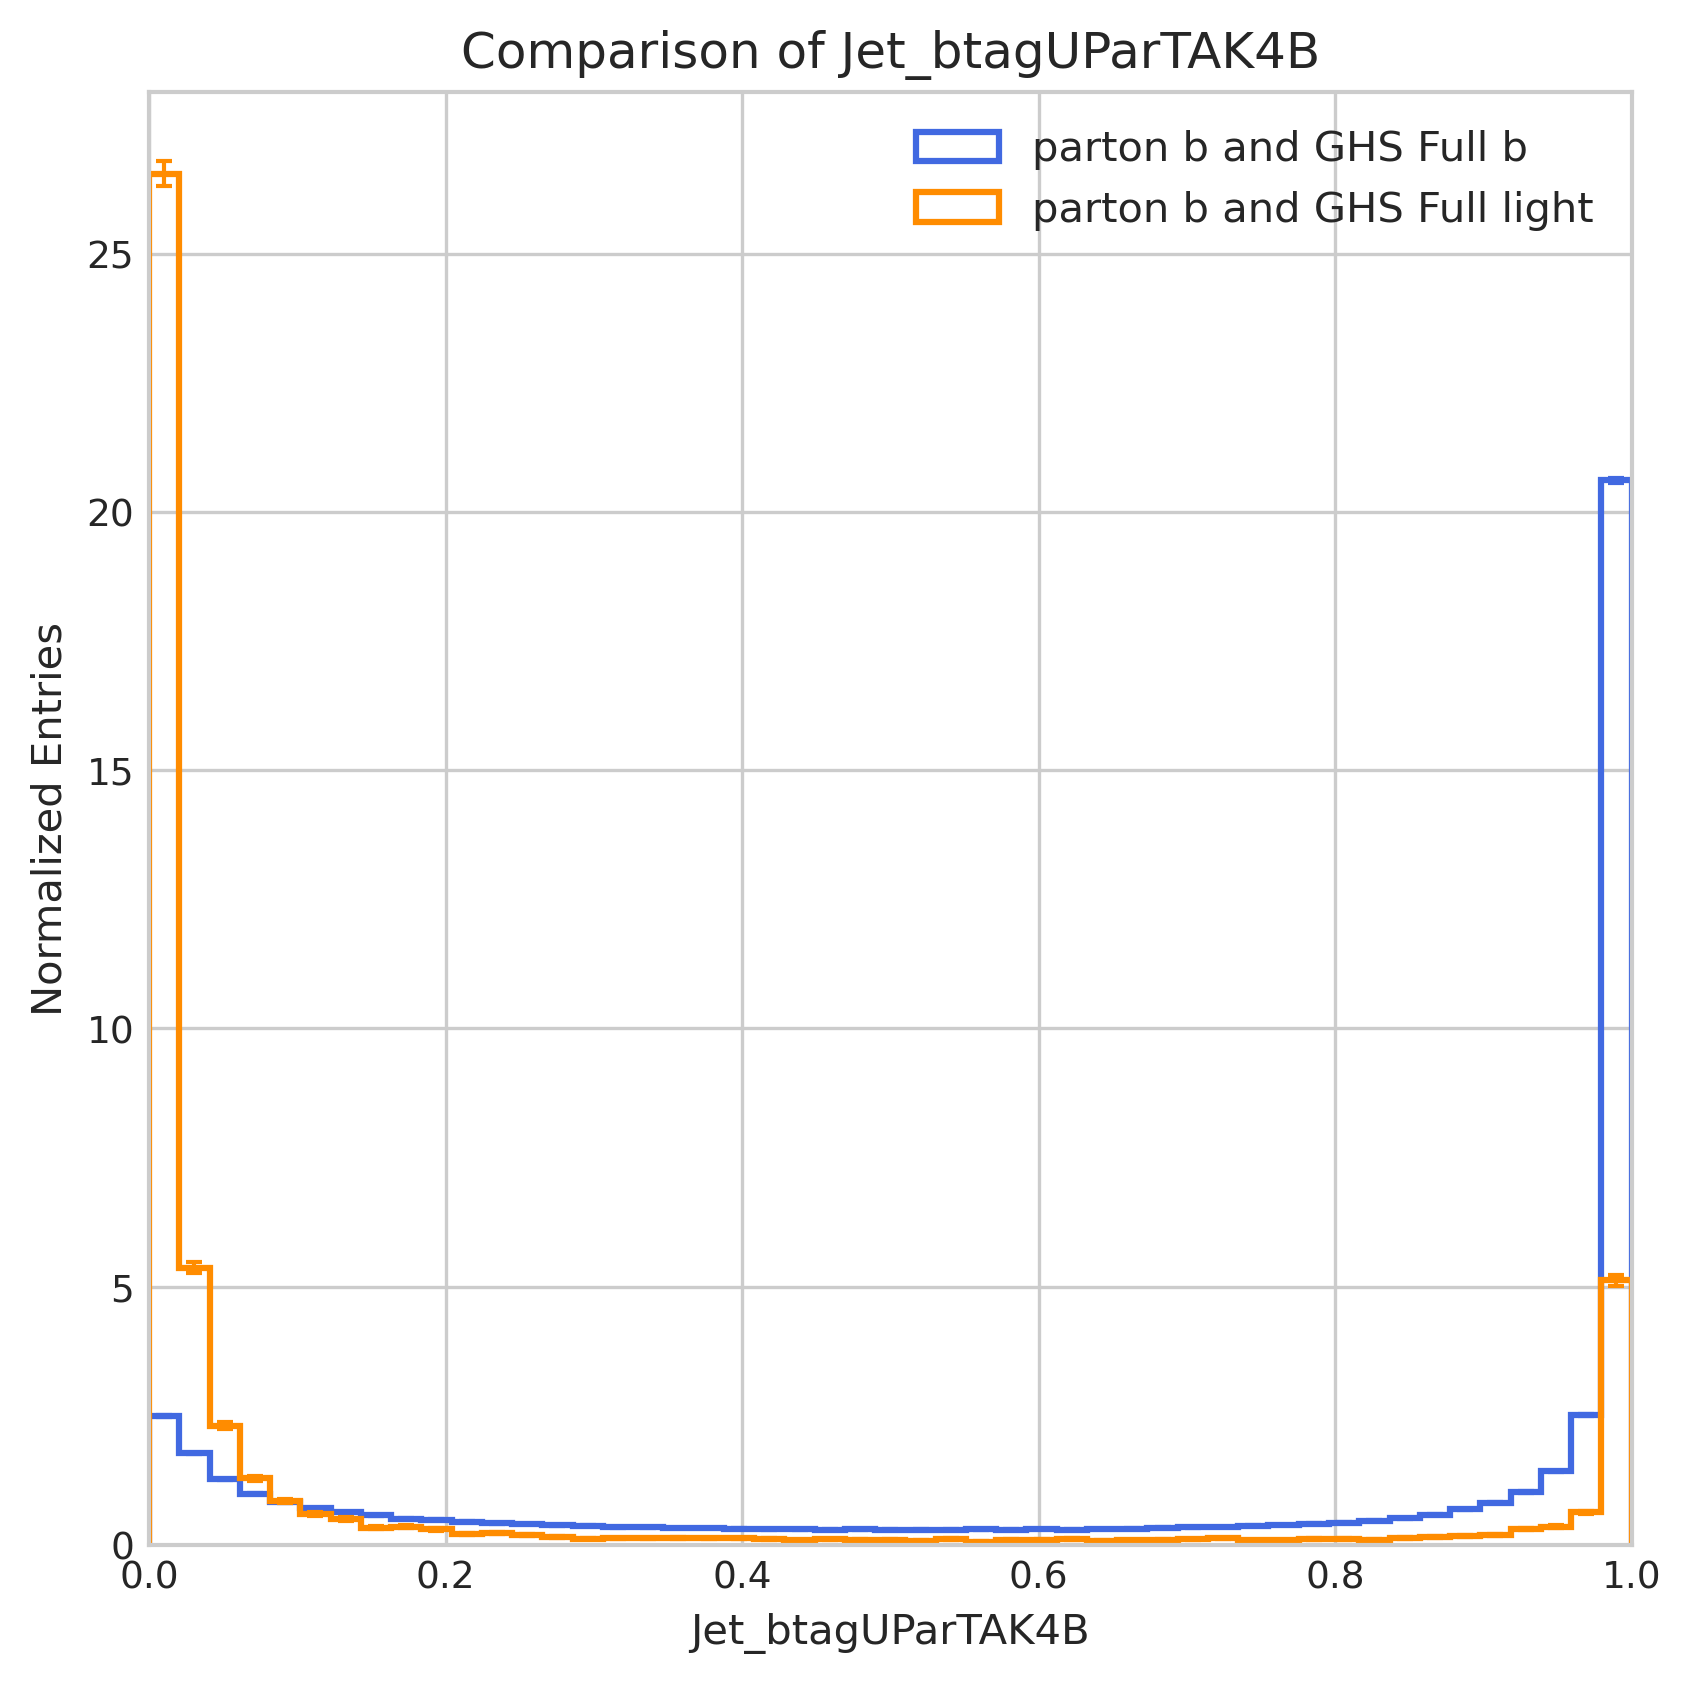
\includegraphics[width=\textwidth]{images/compare_btagUParTAK4B_GHSFull_light_vs_b_filter_partonFlavour_5.png}
        \caption{b-tagging scores from \textsc{ParticleTransformer}}
        \label{fig:jet_btagParT_full_b_parton_b}
    \end{subfigure}
    \caption{Distributions of b-tagging scores for reconstructed jets identified as b-jets by the $\parFlav$ definition. The comparison is between jets also identified as b-flavour by the GHS algorithm (blue) and those classified as light-flavour by GHS (orange). (\subref{fig:jet_btagPNet_full_b_parton_b}) \textsc{ParticleNet} scores; (\subref{fig:jet_btagParT_full_b_parton_b}) \textsc{ParticleTransformer} scores.}
    \label{fig:jet_btag_full_b_parton_b}
\end{figure*}

\begin{figure*}[!htbp]
    \centering
    \begin{subfigure}[t]{0.48\textwidth}
        \centering
        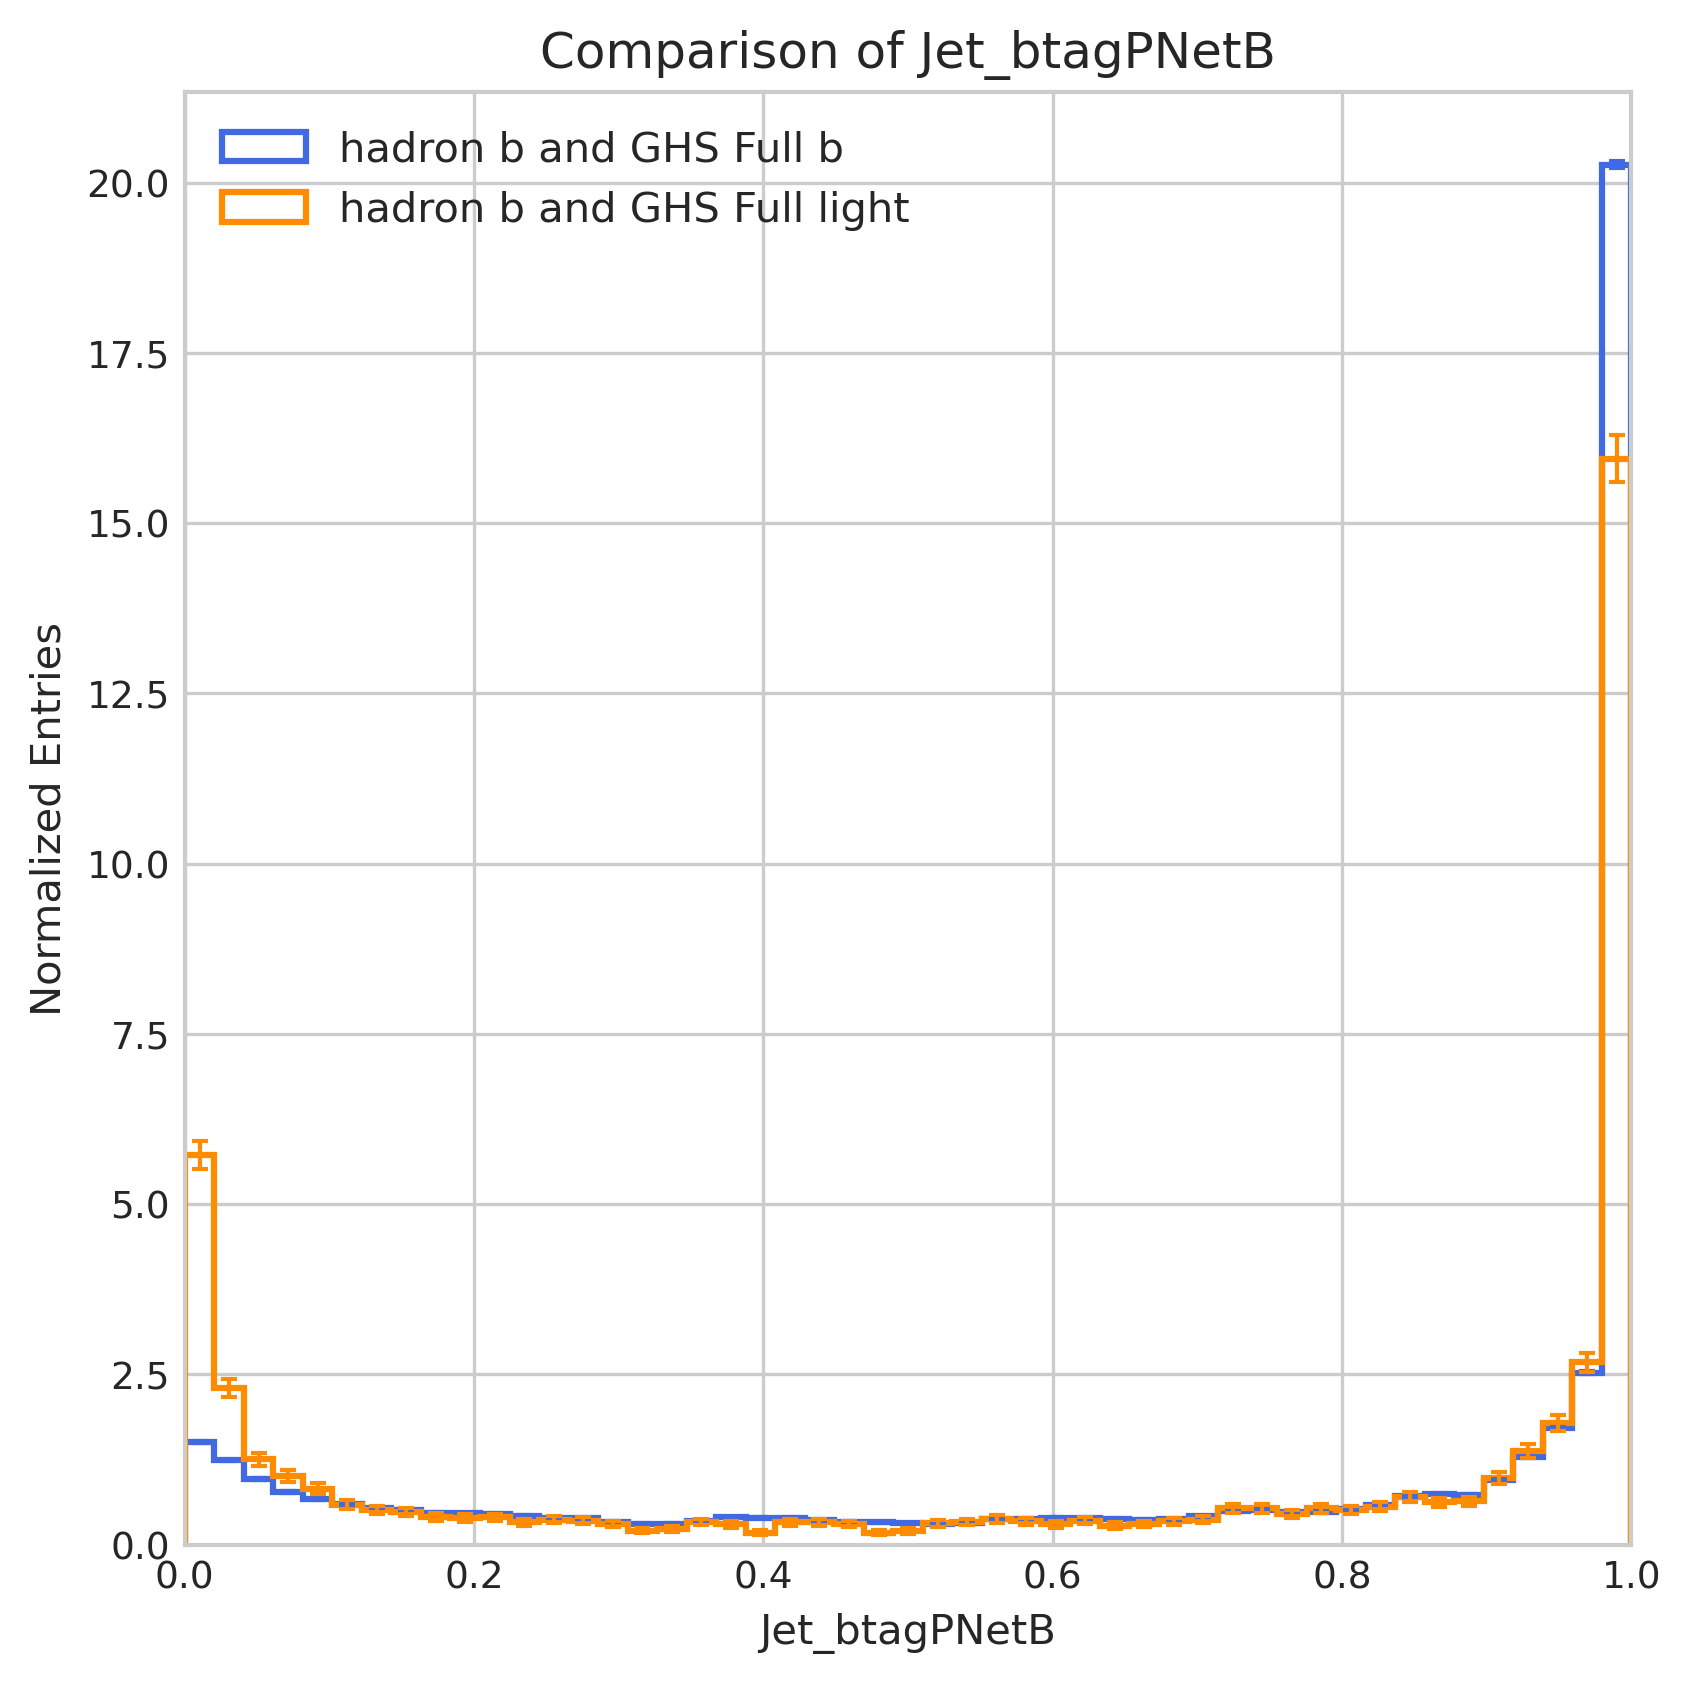
\includegraphics[width=\textwidth]{images/compare_btagPNetB_GHSFull_light_vs_b_filter_hadronFlavour_5.png}
        \caption{b-tagging scores from \textsc{ParticleNet}}
        \label{fig:jet_btagPNet_full_b_hadron_b}
    \end{subfigure}
    \hfill
    \begin{subfigure}[t]{0.48\textwidth}
        \centering
        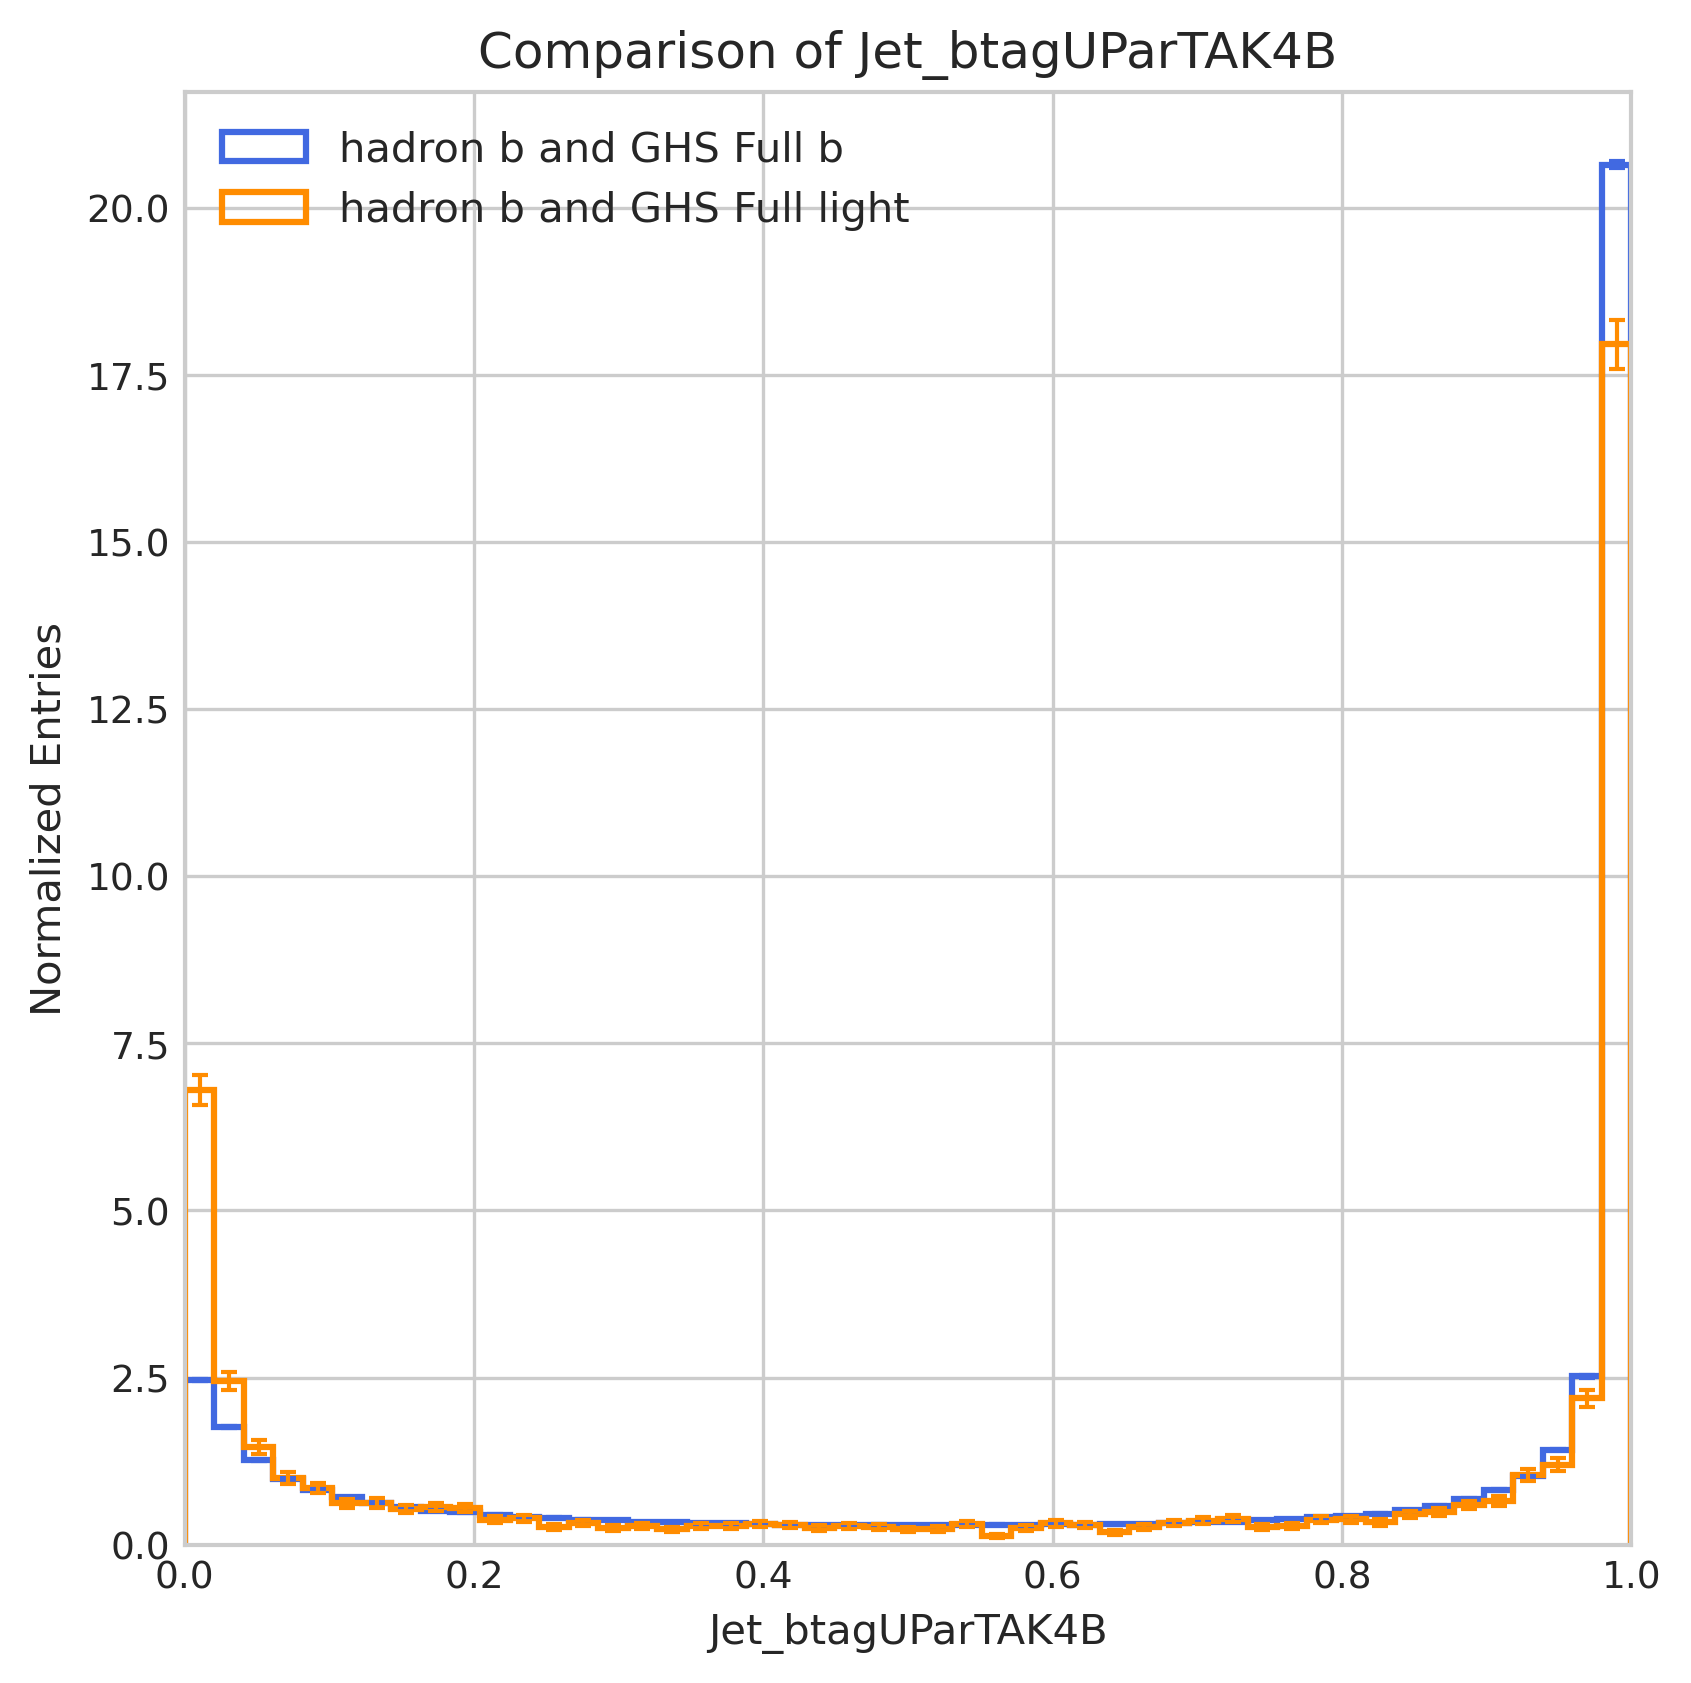
\includegraphics[width=\textwidth]{images/compare_btagUParTAK4B_GHSFull_light_vs_b_filter_hadronFlavour_5.png}
        \caption{b-tagging scores from \textsc{ParticleTransformer}}
        \label{fig:jet_btagParT_full_b_hadron_b}
    \end{subfigure}
    \caption{Distributions of b-tagging scores for reconstructed jets identified as b-jets by the $\hadFlav$ definition. The comparison is between jets also identified as b-flavour by the GHS algorithm (blue) and those classified as light-flavour by GHS (orange). (\subref{fig:jet_btagPNet_full_b_hadron_b}) \textsc{ParticleNet} scores; (\subref{fig:jet_btagParT_full_b_hadron_b}) \textsc{ParticleTransformer} scores.}
    \label{fig:jet_btag_full_b_hadron_b}
\end{figure*}

As is shown from Figure \ref{fig:jet_btag_full_b_parton_b}, light jets defined by GHS but b-jets defined by $\parFlav$ show a peak at tagging scores close to zero, indicating a low likelihood of being b-jets. In contrast, b-jets defined by both GHS and $\parFlav$ show a significantly higher proportion of jets tagging scores close to one. Such trends are less pronounced in Figure \ref{fig:jet_btag_full_b_parton_b} where jets initially defined as b-jets by $\hadFlav$ are compared, in line with the fact that both \textsc{ParticleNet} and \textsc{ParticleTransformer} are trained based on jets labeled with $\hadFlav$ \cite{CMS-PAS-BTV-22-001}, and still suggesting that the jets labeled by GHS algorithm are more likely genuine b-jets.

\section{Summary and Outlook} %[TODO]
\label{sec:sum}

\subsection{Summary of Work and Pending Approval}
\label{sec:sum-summary}

This project has successfully integrated the IRC-safe GHS jet flavour algorithm into the CMSSW framework. Key achievements include the interfacing of the external$\texttt{fastjet-contrib}$ library, the development of a ghost-clustering method for parton-jet association, the design of a compact NanoAOD storage format, and a comprehensive validation demonstrating the algorithm's physical robustness. The code has been developed in a public branch and is being prepared for a pull request for inclusion in an official CMSSW release. The work and preliminary results were recently presented at the CMS B-Tagging and Vertexing (BTV) group software meeting.

\subsection{Outlook: Retraining Flavour Tagging Models} %[TODO]
\label{sec:sum-outlook}

The ultimate goal of this work is to provide a theoretically sound basis for jet flavour identification at CMS. The next crucial step will be to use the GHS flavour labels, produced in large-scale Monte Carlo simulations, as the "ground truth" for training the latest generation of machine learning-based flavour tagging models (e.g., \textsc{DeepJet}, \textsc{ParticleTransformer}). By training on an IRC-safe definition, it is expected that the resulting taggers will allow comparison with theory at higher orders, offering reduced systematic uncertainties and more precise physics measurements in Run 3 and beyond. This work provides the essential technical foundation for that future program.

\printbibliography
\end{document}
